% Options for packages loaded elsewhere
\PassOptionsToPackage{unicode}{hyperref}
\PassOptionsToPackage{hyphens}{url}
\PassOptionsToPackage{dvipsnames,svgnames,x11names}{xcolor}
%
\documentclass[
]{article}
\usepackage{amsmath,amssymb}
\usepackage{lmodern}
\usepackage{iftex}
\ifPDFTeX
  \usepackage[T1]{fontenc}
  \usepackage[utf8]{inputenc}
  \usepackage{textcomp} % provide euro and other symbols
\else % if luatex or xetex
  \usepackage{unicode-math}
  \defaultfontfeatures{Scale=MatchLowercase}
  \defaultfontfeatures[\rmfamily]{Ligatures=TeX,Scale=1}
\fi
% Use upquote if available, for straight quotes in verbatim environments
\IfFileExists{upquote.sty}{\usepackage{upquote}}{}
\IfFileExists{microtype.sty}{% use microtype if available
  \usepackage[]{microtype}
  \UseMicrotypeSet[protrusion]{basicmath} % disable protrusion for tt fonts
}{}
\makeatletter
\@ifundefined{KOMAClassName}{% if non-KOMA class
  \IfFileExists{parskip.sty}{%
    \usepackage{parskip}
  }{% else
    \setlength{\parindent}{0pt}
    \setlength{\parskip}{6pt plus 2pt minus 1pt}}
}{% if KOMA class
  \KOMAoptions{parskip=half}}
\makeatother
\usepackage{xcolor}
\IfFileExists{xurl.sty}{\usepackage{xurl}}{} % add URL line breaks if available
\IfFileExists{bookmark.sty}{\usepackage{bookmark}}{\usepackage{hyperref}}
\hypersetup{
  pdftitle={BDA - Assignment 9},
  pdfauthor={Anonymous},
  colorlinks=true,
  linkcolor={Maroon},
  filecolor={Maroon},
  citecolor={Blue},
  urlcolor={blue},
  pdfcreator={LaTeX via pandoc}}
\urlstyle{same} % disable monospaced font for URLs
\usepackage[margin=1in]{geometry}
\usepackage{color}
\usepackage{fancyvrb}
\newcommand{\VerbBar}{|}
\newcommand{\VERB}{\Verb[commandchars=\\\{\}]}
\DefineVerbatimEnvironment{Highlighting}{Verbatim}{commandchars=\\\{\}}
% Add ',fontsize=\small' for more characters per line
\usepackage{framed}
\definecolor{shadecolor}{RGB}{248,248,248}
\newenvironment{Shaded}{\begin{snugshade}}{\end{snugshade}}
\newcommand{\AlertTok}[1]{\textcolor[rgb]{0.94,0.16,0.16}{#1}}
\newcommand{\AnnotationTok}[1]{\textcolor[rgb]{0.56,0.35,0.01}{\textbf{\textit{#1}}}}
\newcommand{\AttributeTok}[1]{\textcolor[rgb]{0.77,0.63,0.00}{#1}}
\newcommand{\BaseNTok}[1]{\textcolor[rgb]{0.00,0.00,0.81}{#1}}
\newcommand{\BuiltInTok}[1]{#1}
\newcommand{\CharTok}[1]{\textcolor[rgb]{0.31,0.60,0.02}{#1}}
\newcommand{\CommentTok}[1]{\textcolor[rgb]{0.56,0.35,0.01}{\textit{#1}}}
\newcommand{\CommentVarTok}[1]{\textcolor[rgb]{0.56,0.35,0.01}{\textbf{\textit{#1}}}}
\newcommand{\ConstantTok}[1]{\textcolor[rgb]{0.00,0.00,0.00}{#1}}
\newcommand{\ControlFlowTok}[1]{\textcolor[rgb]{0.13,0.29,0.53}{\textbf{#1}}}
\newcommand{\DataTypeTok}[1]{\textcolor[rgb]{0.13,0.29,0.53}{#1}}
\newcommand{\DecValTok}[1]{\textcolor[rgb]{0.00,0.00,0.81}{#1}}
\newcommand{\DocumentationTok}[1]{\textcolor[rgb]{0.56,0.35,0.01}{\textbf{\textit{#1}}}}
\newcommand{\ErrorTok}[1]{\textcolor[rgb]{0.64,0.00,0.00}{\textbf{#1}}}
\newcommand{\ExtensionTok}[1]{#1}
\newcommand{\FloatTok}[1]{\textcolor[rgb]{0.00,0.00,0.81}{#1}}
\newcommand{\FunctionTok}[1]{\textcolor[rgb]{0.00,0.00,0.00}{#1}}
\newcommand{\ImportTok}[1]{#1}
\newcommand{\InformationTok}[1]{\textcolor[rgb]{0.56,0.35,0.01}{\textbf{\textit{#1}}}}
\newcommand{\KeywordTok}[1]{\textcolor[rgb]{0.13,0.29,0.53}{\textbf{#1}}}
\newcommand{\NormalTok}[1]{#1}
\newcommand{\OperatorTok}[1]{\textcolor[rgb]{0.81,0.36,0.00}{\textbf{#1}}}
\newcommand{\OtherTok}[1]{\textcolor[rgb]{0.56,0.35,0.01}{#1}}
\newcommand{\PreprocessorTok}[1]{\textcolor[rgb]{0.56,0.35,0.01}{\textit{#1}}}
\newcommand{\RegionMarkerTok}[1]{#1}
\newcommand{\SpecialCharTok}[1]{\textcolor[rgb]{0.00,0.00,0.00}{#1}}
\newcommand{\SpecialStringTok}[1]{\textcolor[rgb]{0.31,0.60,0.02}{#1}}
\newcommand{\StringTok}[1]{\textcolor[rgb]{0.31,0.60,0.02}{#1}}
\newcommand{\VariableTok}[1]{\textcolor[rgb]{0.00,0.00,0.00}{#1}}
\newcommand{\VerbatimStringTok}[1]{\textcolor[rgb]{0.31,0.60,0.02}{#1}}
\newcommand{\WarningTok}[1]{\textcolor[rgb]{0.56,0.35,0.01}{\textbf{\textit{#1}}}}
\usepackage{graphicx}
\makeatletter
\def\maxwidth{\ifdim\Gin@nat@width>\linewidth\linewidth\else\Gin@nat@width\fi}
\def\maxheight{\ifdim\Gin@nat@height>\textheight\textheight\else\Gin@nat@height\fi}
\makeatother
% Scale images if necessary, so that they will not overflow the page
% margins by default, and it is still possible to overwrite the defaults
% using explicit options in \includegraphics[width, height, ...]{}
\setkeys{Gin}{width=\maxwidth,height=\maxheight,keepaspectratio}
% Set default figure placement to htbp
\makeatletter
\def\fps@figure{htbp}
\makeatother
\setlength{\emergencystretch}{3em} % prevent overfull lines
\providecommand{\tightlist}{%
  \setlength{\itemsep}{0pt}\setlength{\parskip}{0pt}}
\setcounter{secnumdepth}{-\maxdimen} % remove section numbering
\newlength{\cslhangindent}
\setlength{\cslhangindent}{1.5em}
\newlength{\csllabelwidth}
\setlength{\csllabelwidth}{3em}
\newlength{\cslentryspacingunit} % times entry-spacing
\setlength{\cslentryspacingunit}{\parskip}
\newenvironment{CSLReferences}[2] % #1 hanging-ident, #2 entry spacing
 {% don't indent paragraphs
  \setlength{\parindent}{0pt}
  % turn on hanging indent if param 1 is 1
  \ifodd #1
  \let\oldpar\par
  \def\par{\hangindent=\cslhangindent\oldpar}
  \fi
  % set entry spacing
  \setlength{\parskip}{#2\cslentryspacingunit}
 }%
 {}
\usepackage{calc}
\newcommand{\CSLBlock}[1]{#1\hfill\break}
\newcommand{\CSLLeftMargin}[1]{\parbox[t]{\csllabelwidth}{#1}}
\newcommand{\CSLRightInline}[1]{\parbox[t]{\linewidth - \csllabelwidth}{#1}\break}
\newcommand{\CSLIndent}[1]{\hspace{\cslhangindent}#1}
\usepackage{listings}
\ifLuaTeX
  \usepackage{selnolig}  % disable illegal ligatures
\fi

\title{BDA - Assignment 9}
\author{Anonymous}
\date{}

\begin{document}
\maketitle

{
\hypersetup{linkcolor=}
\setcounter{tocdepth}{1}
\tableofcontents
}
\hypertarget{introduction}{%
\section{1. Introduction}\label{introduction}}

It's been almost 2 years since the covid-19 started in December 2019,
and it's been 1 year since world vaccination has been started December
2020. Even though most of the countries rushing into vaccination and
some countries are picking over 80\% rate in vaccination, the pandemic
seems unstoppable. One of the popular idea to stop the pandemic is that
to achieve a 'herd-immunity threshold, which occurs when a large portion
of a community (the herd) becomes immune to a disease, making the spread
of disease from person to person unlikely. Immune individuals are
unlikely to contribute to disease transmission, disrupting chains of
infection, which stops or slows the spread of disease {``Herd
Immunity''} (n.d.). It is known that the herd-immunity threshold is
achievable only with high vaccination rates, and many scientists had
thought that once people started being immunized en masse, herd immunity
would permit society to return to normal. Most estimates had placed the
threshold at 60--70\% of the population gaining immunity, either through
vaccinations or past exposure to the virus {``Five Reasons Why COVID
Herd Immunity Is Probably Impossible''} (n.d.). Down below shows the
graph of population fully vaccinated by countries.

\begin{Shaded}
\begin{Highlighting}[]
\NormalTok{knitr}\SpecialCharTok{::}\FunctionTok{include\_graphics}\NormalTok{(}\StringTok{"./image/share{-}people{-}fully{-}vaccinated{-}covid\_world.png"}\NormalTok{)}
\end{Highlighting}
\end{Shaded}

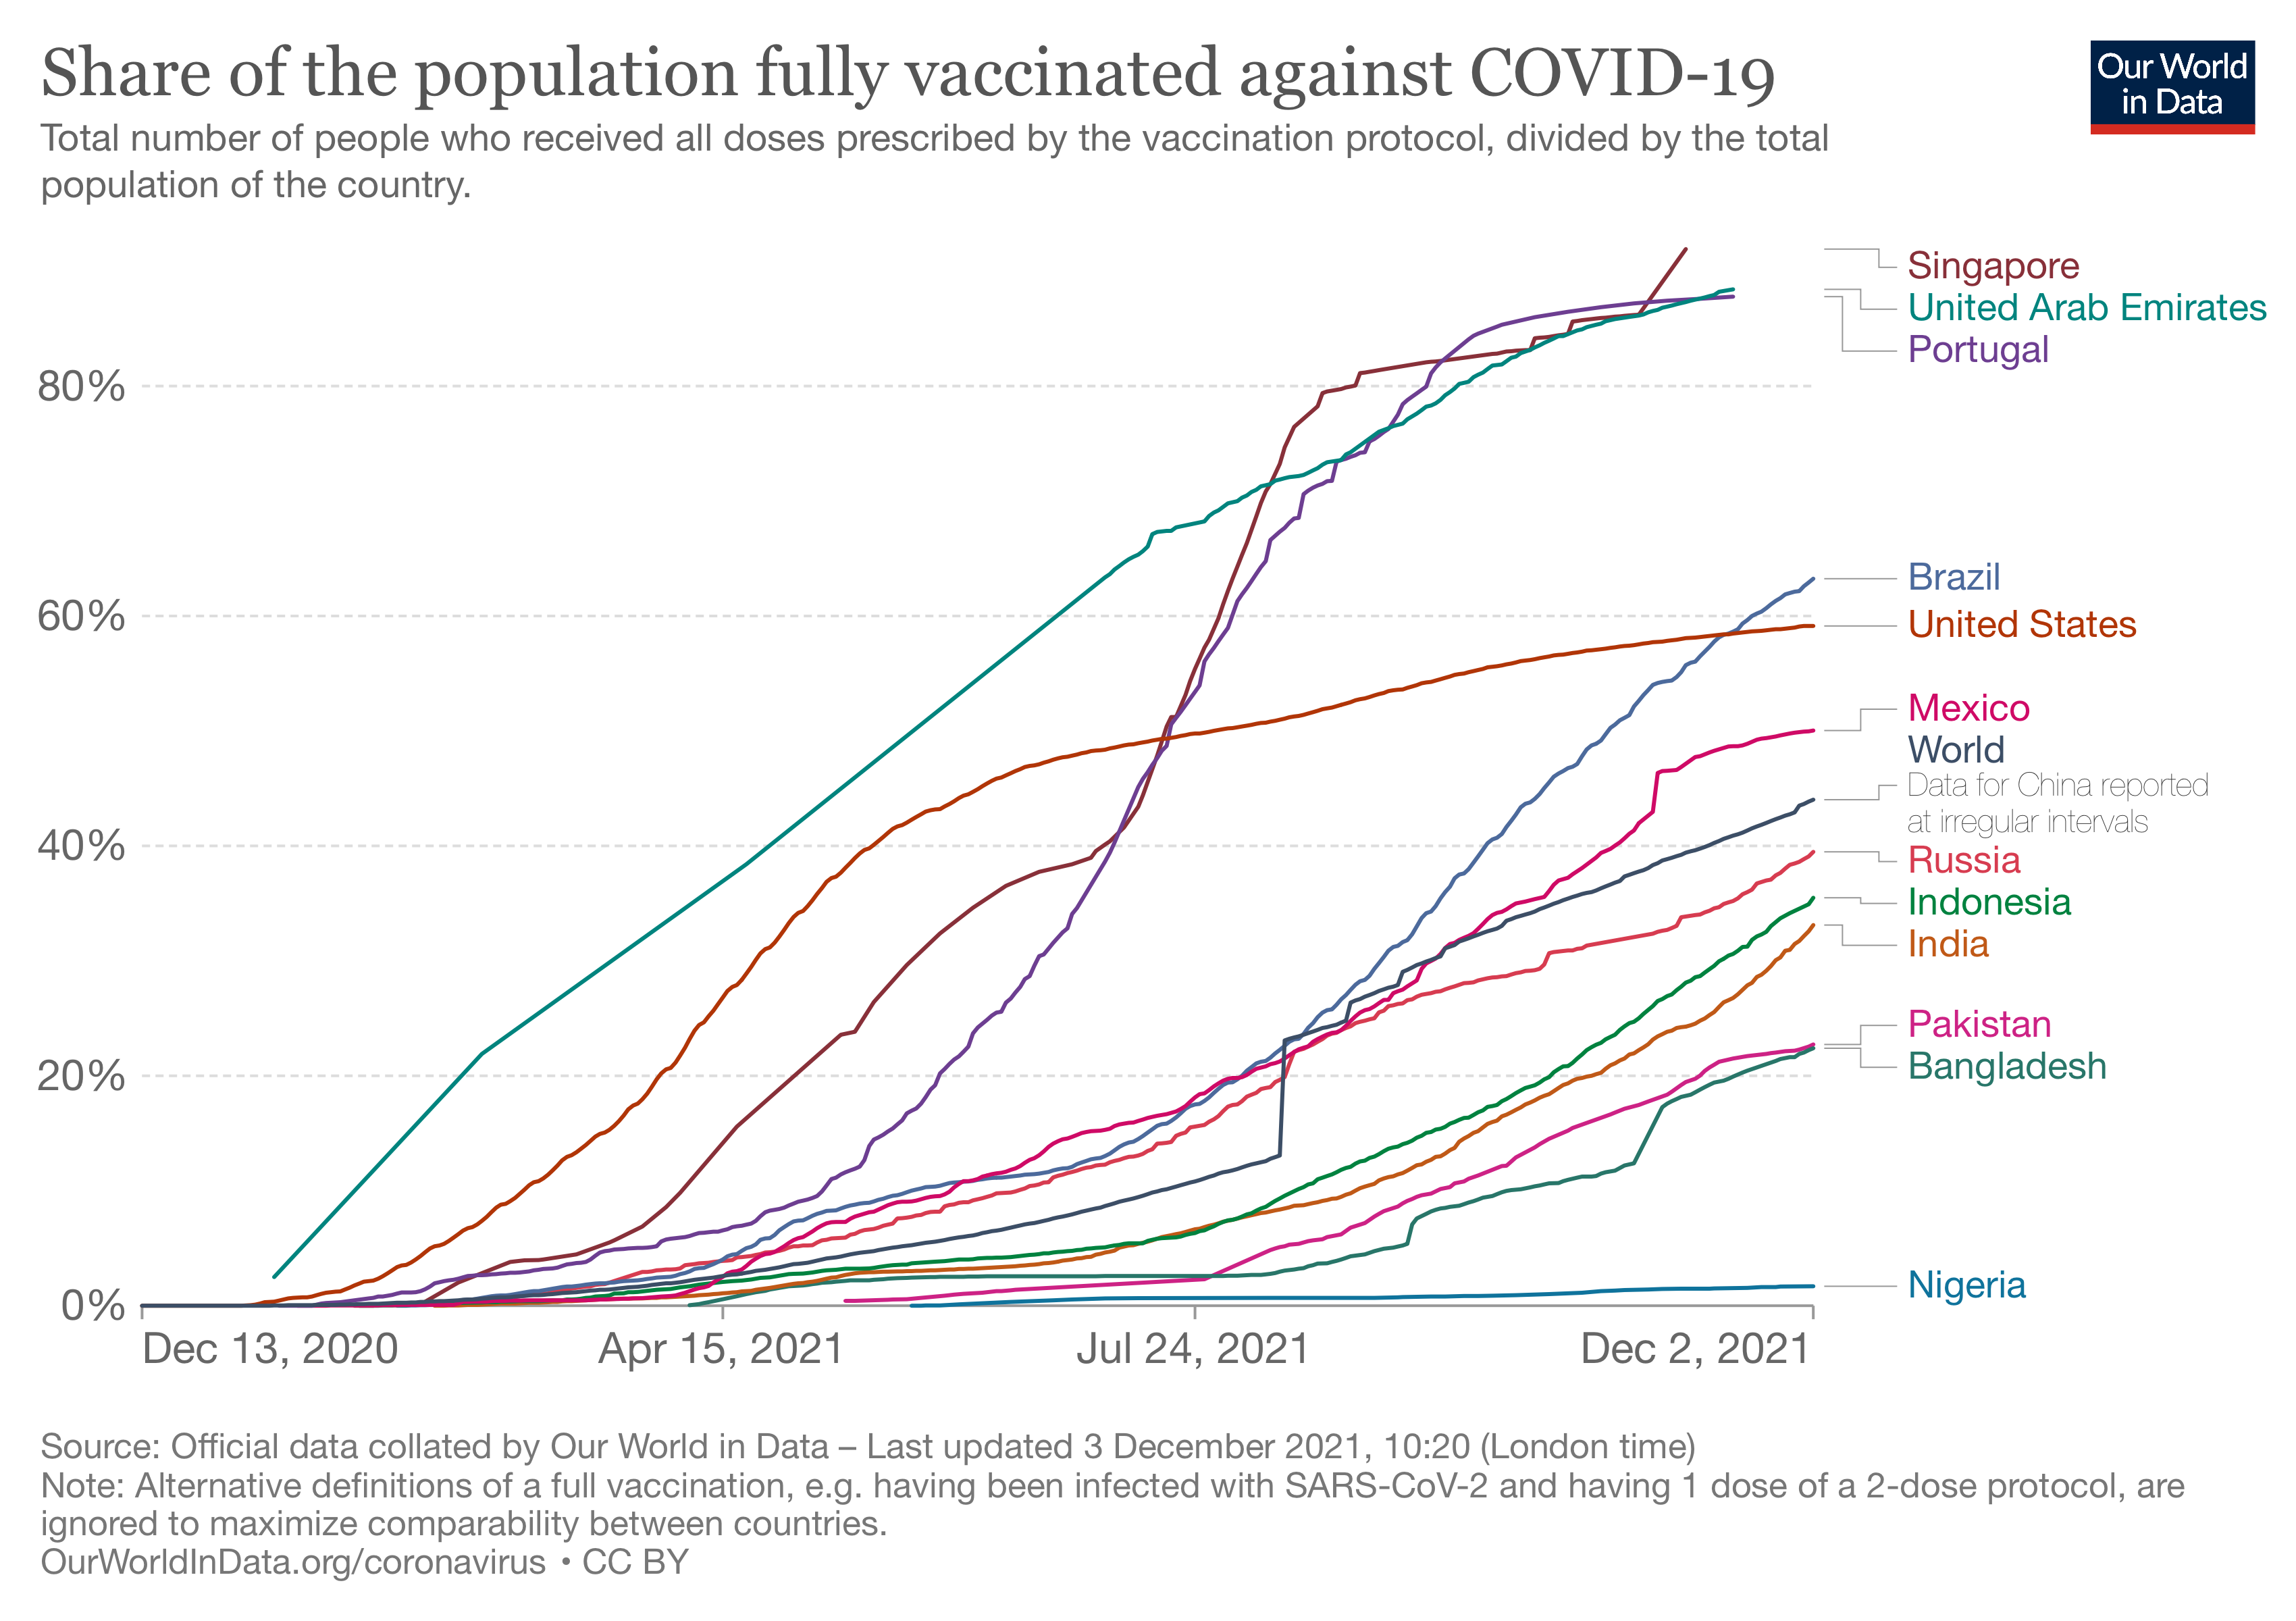
\includegraphics{./image/share-people-fully-vaccinated-covid_world.png}

As the high vaccination rate is a big part of ending pandemic by
achieving herd-immunity, our group was interested in predicting how much
high vaccination rate that countries will achieve in future. As we
expect the cumulative vaccination rate graph will follow logit function,
we set our model as a logit function. We picked 5 countries,which are
Finland, Portugal, Japan, Germany,and Hongkong for our data. The
cumulative vaccination graphs in these countries roughly follow the
logit function and our main modeling idea is to see find which model the
data fits well (seperate model or hierarchical model) and to predict the
future vaccination rate.

Down below shows the barplot of population rate who received at least
one dose of covid19 vaccine by countries in our interest.

\begin{Shaded}
\begin{Highlighting}[]
\NormalTok{knitr}\SpecialCharTok{::}\FunctionTok{include\_graphics}\NormalTok{(}\StringTok{"./image/share{-}people{-}vaccinated{-}covid.png"}\NormalTok{)}
\end{Highlighting}
\end{Shaded}

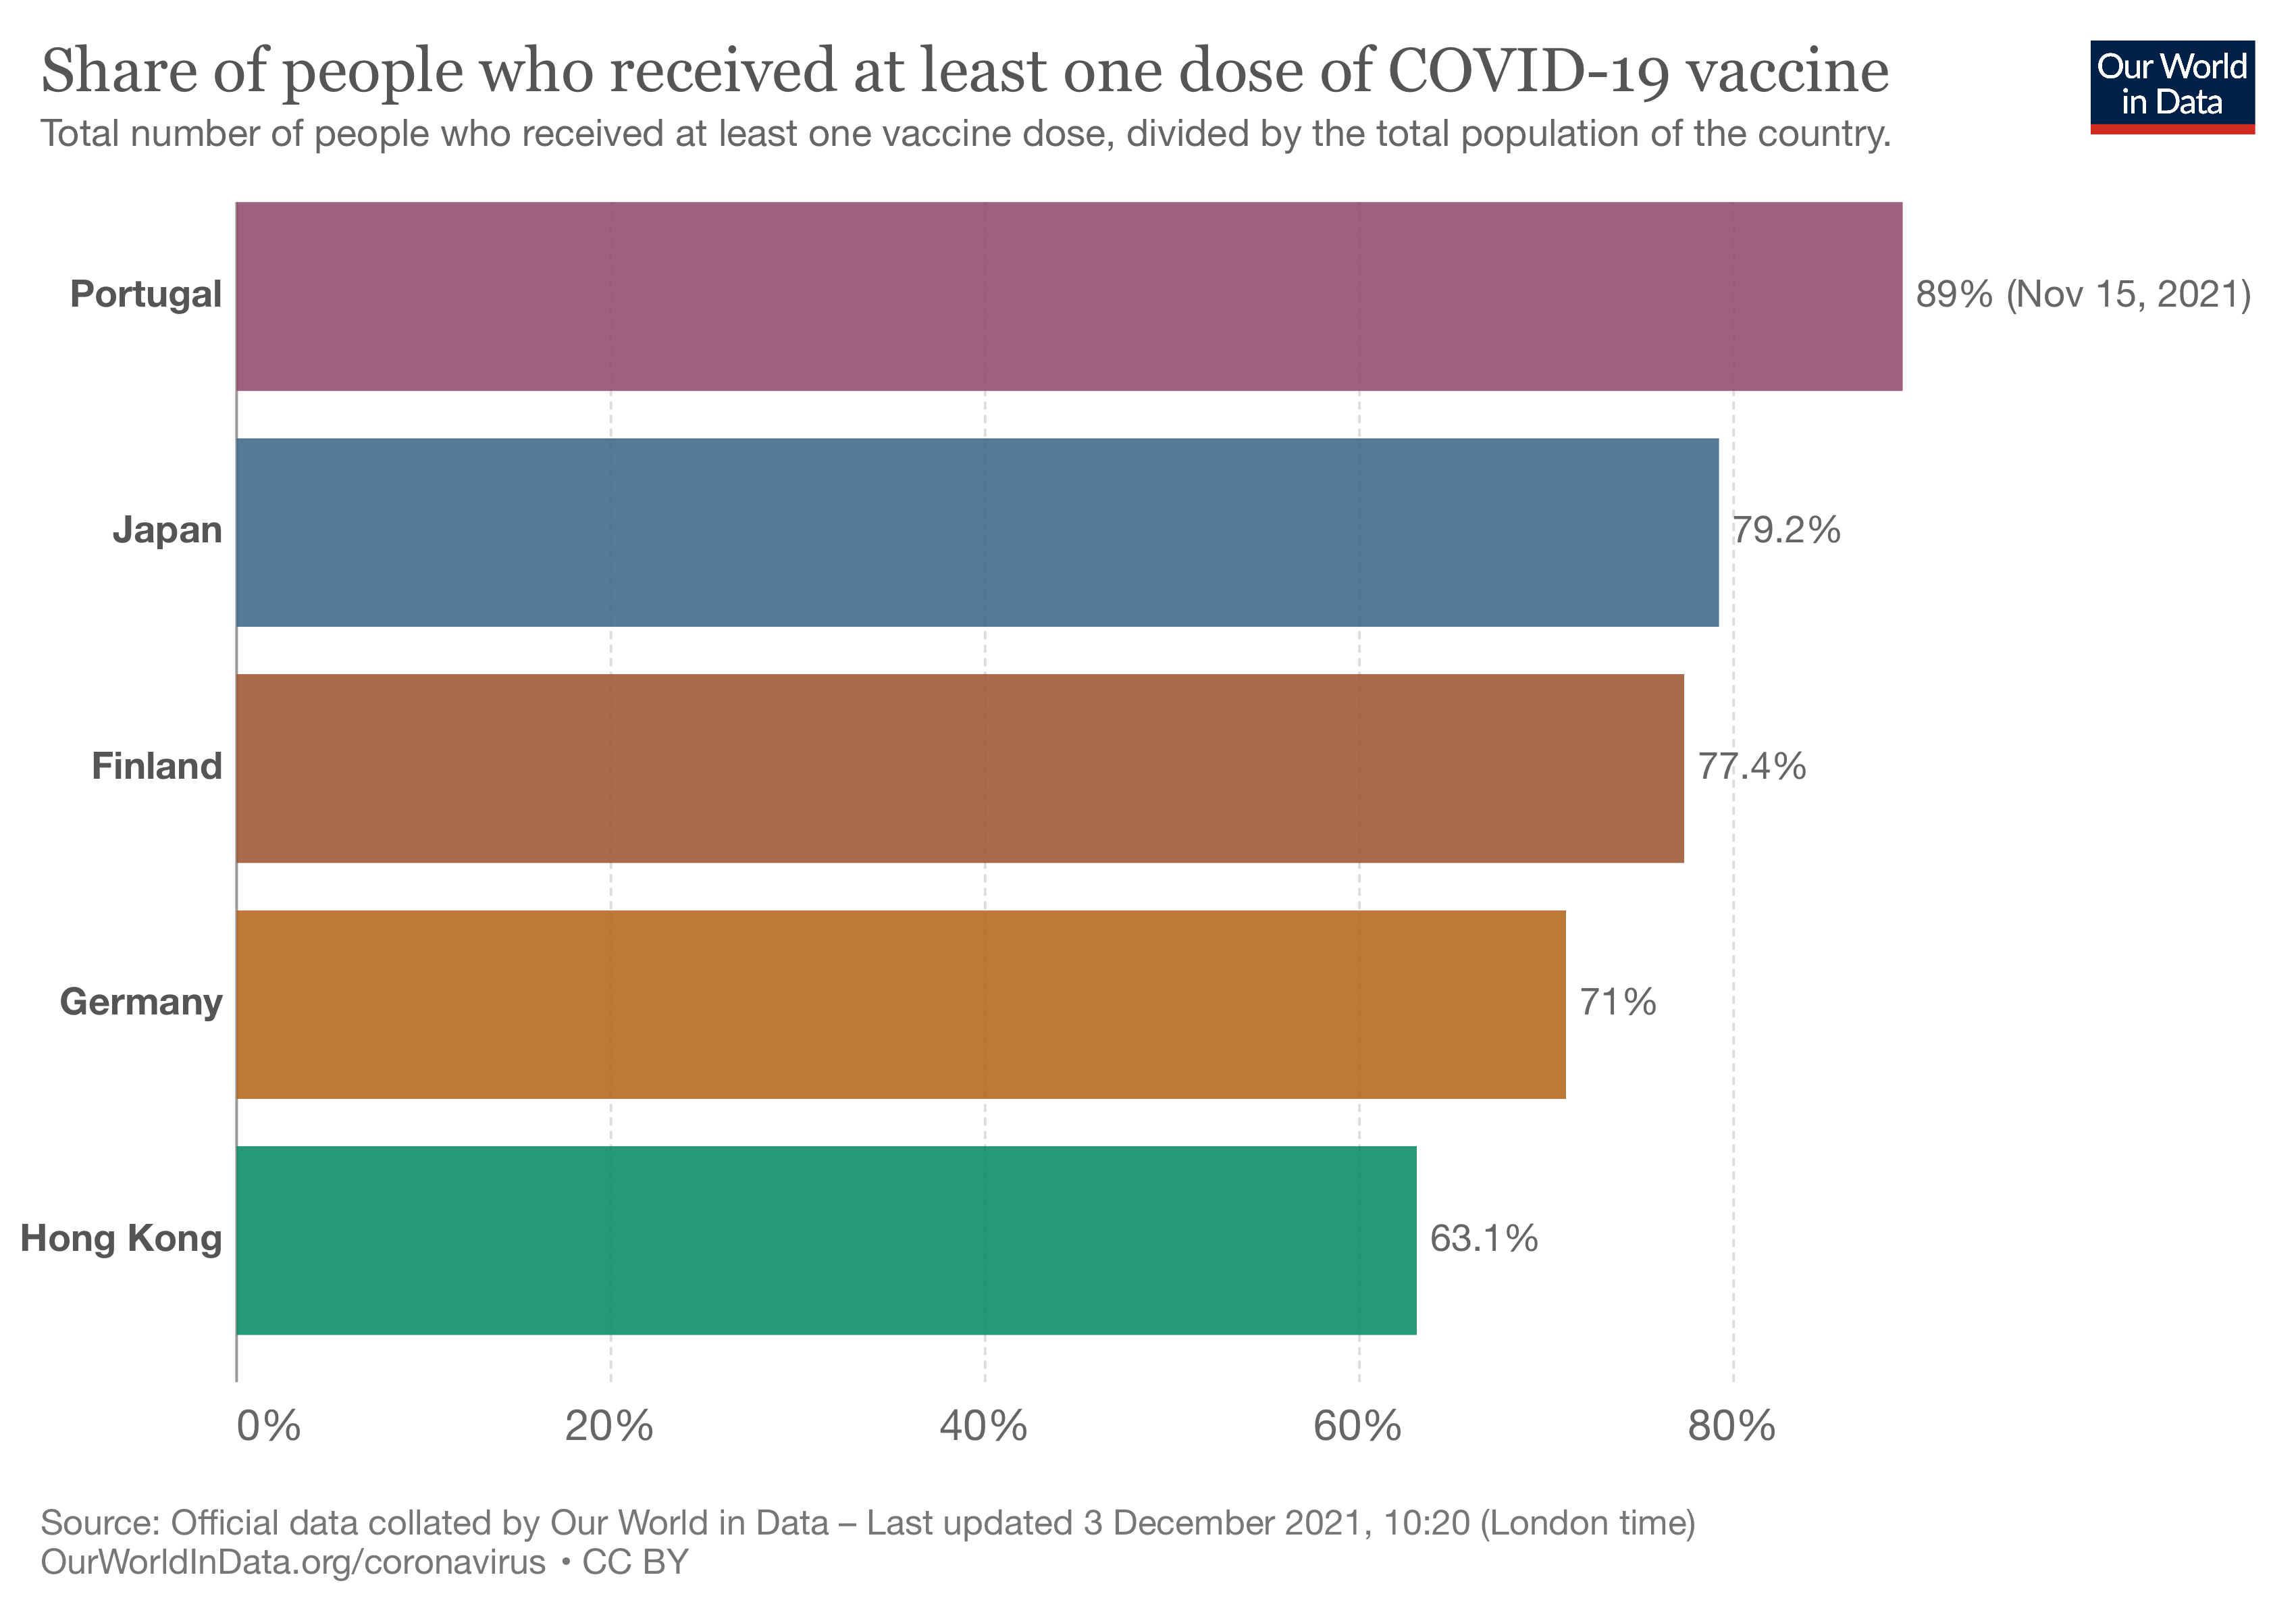
\includegraphics{./image/share-people-vaccinated-covid.png}

Down below shows the barplot of population rate of fully vaccinated
against covid19 by countries in our interest.

\begin{Shaded}
\begin{Highlighting}[]
\NormalTok{knitr}\SpecialCharTok{::}\FunctionTok{include\_graphics}\NormalTok{(}\StringTok{"./image/share{-}people{-}fully{-}vaccinated{-}covid\_bar.png"}\NormalTok{)}
\end{Highlighting}
\end{Shaded}

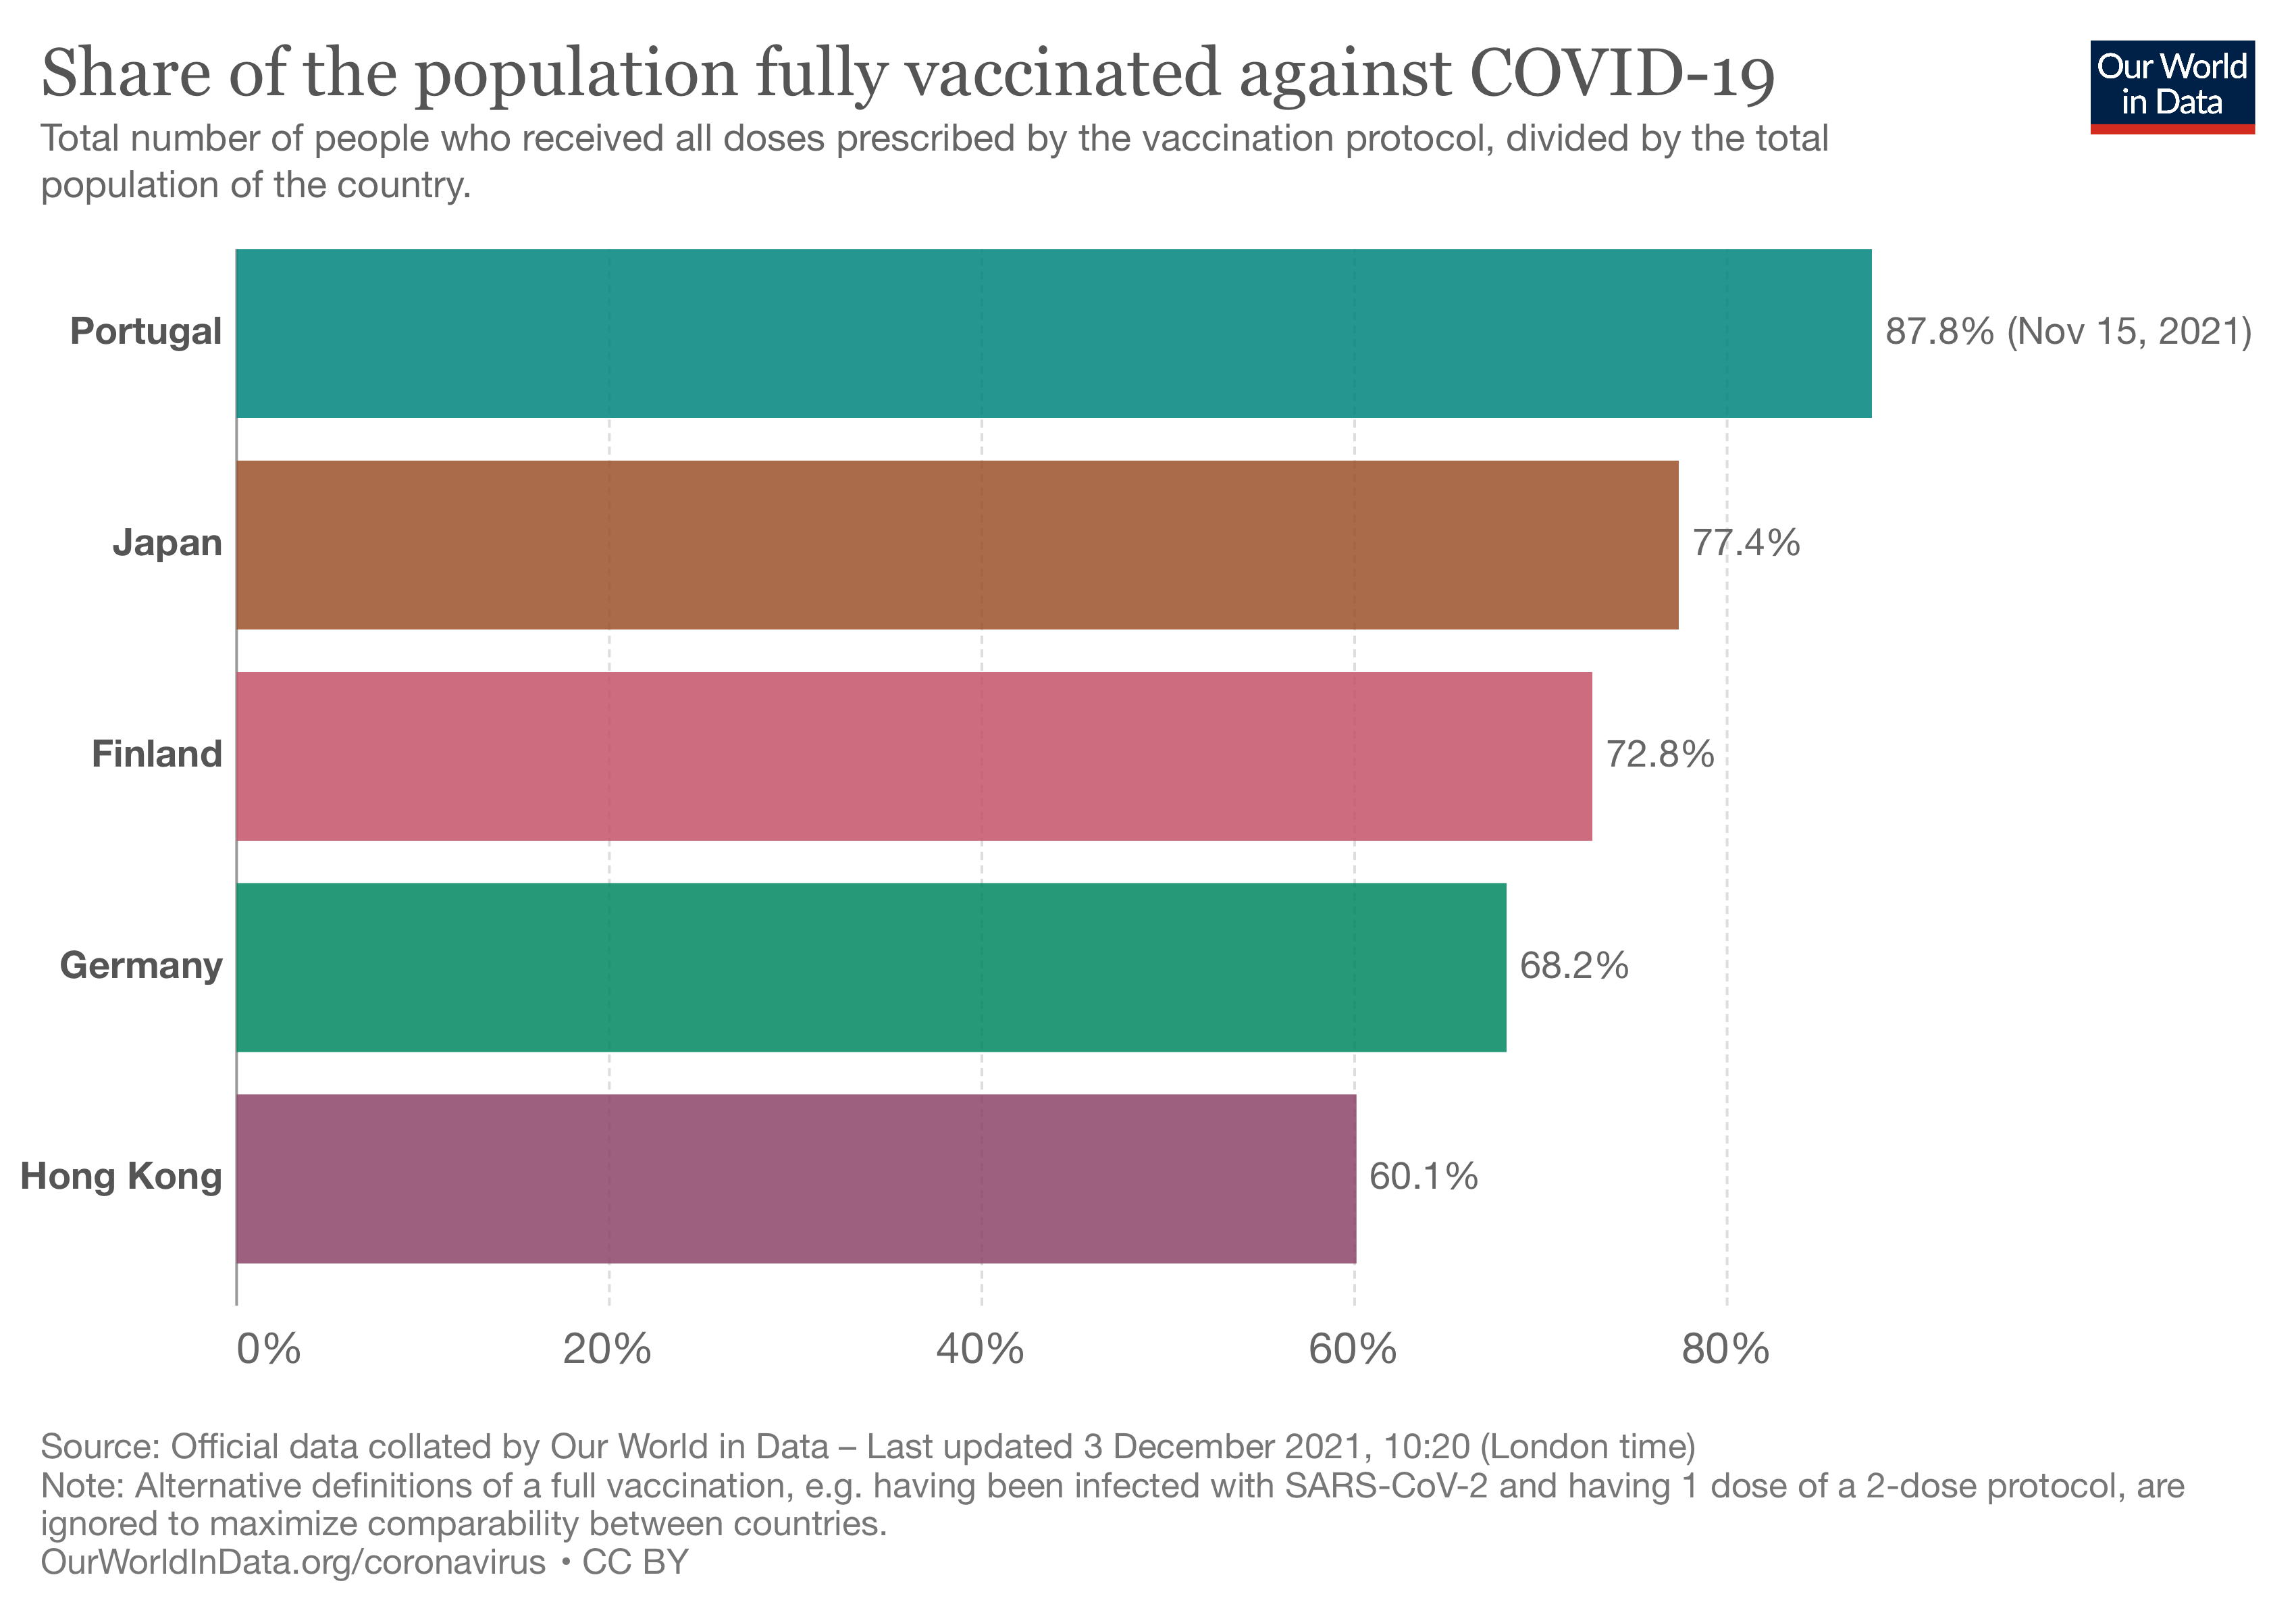
\includegraphics{./image/share-people-fully-vaccinated-covid_bar.png}

Down below shows the barplot of fully vaccinated population rate by
countries in our interest.

\begin{Shaded}
\begin{Highlighting}[]
\NormalTok{knitr}\SpecialCharTok{::}\FunctionTok{include\_graphics}\NormalTok{(}\StringTok{"./image/share{-}people{-}fully{-}vaccinated{-}covid\_plot.png"}\NormalTok{)}
\end{Highlighting}
\end{Shaded}

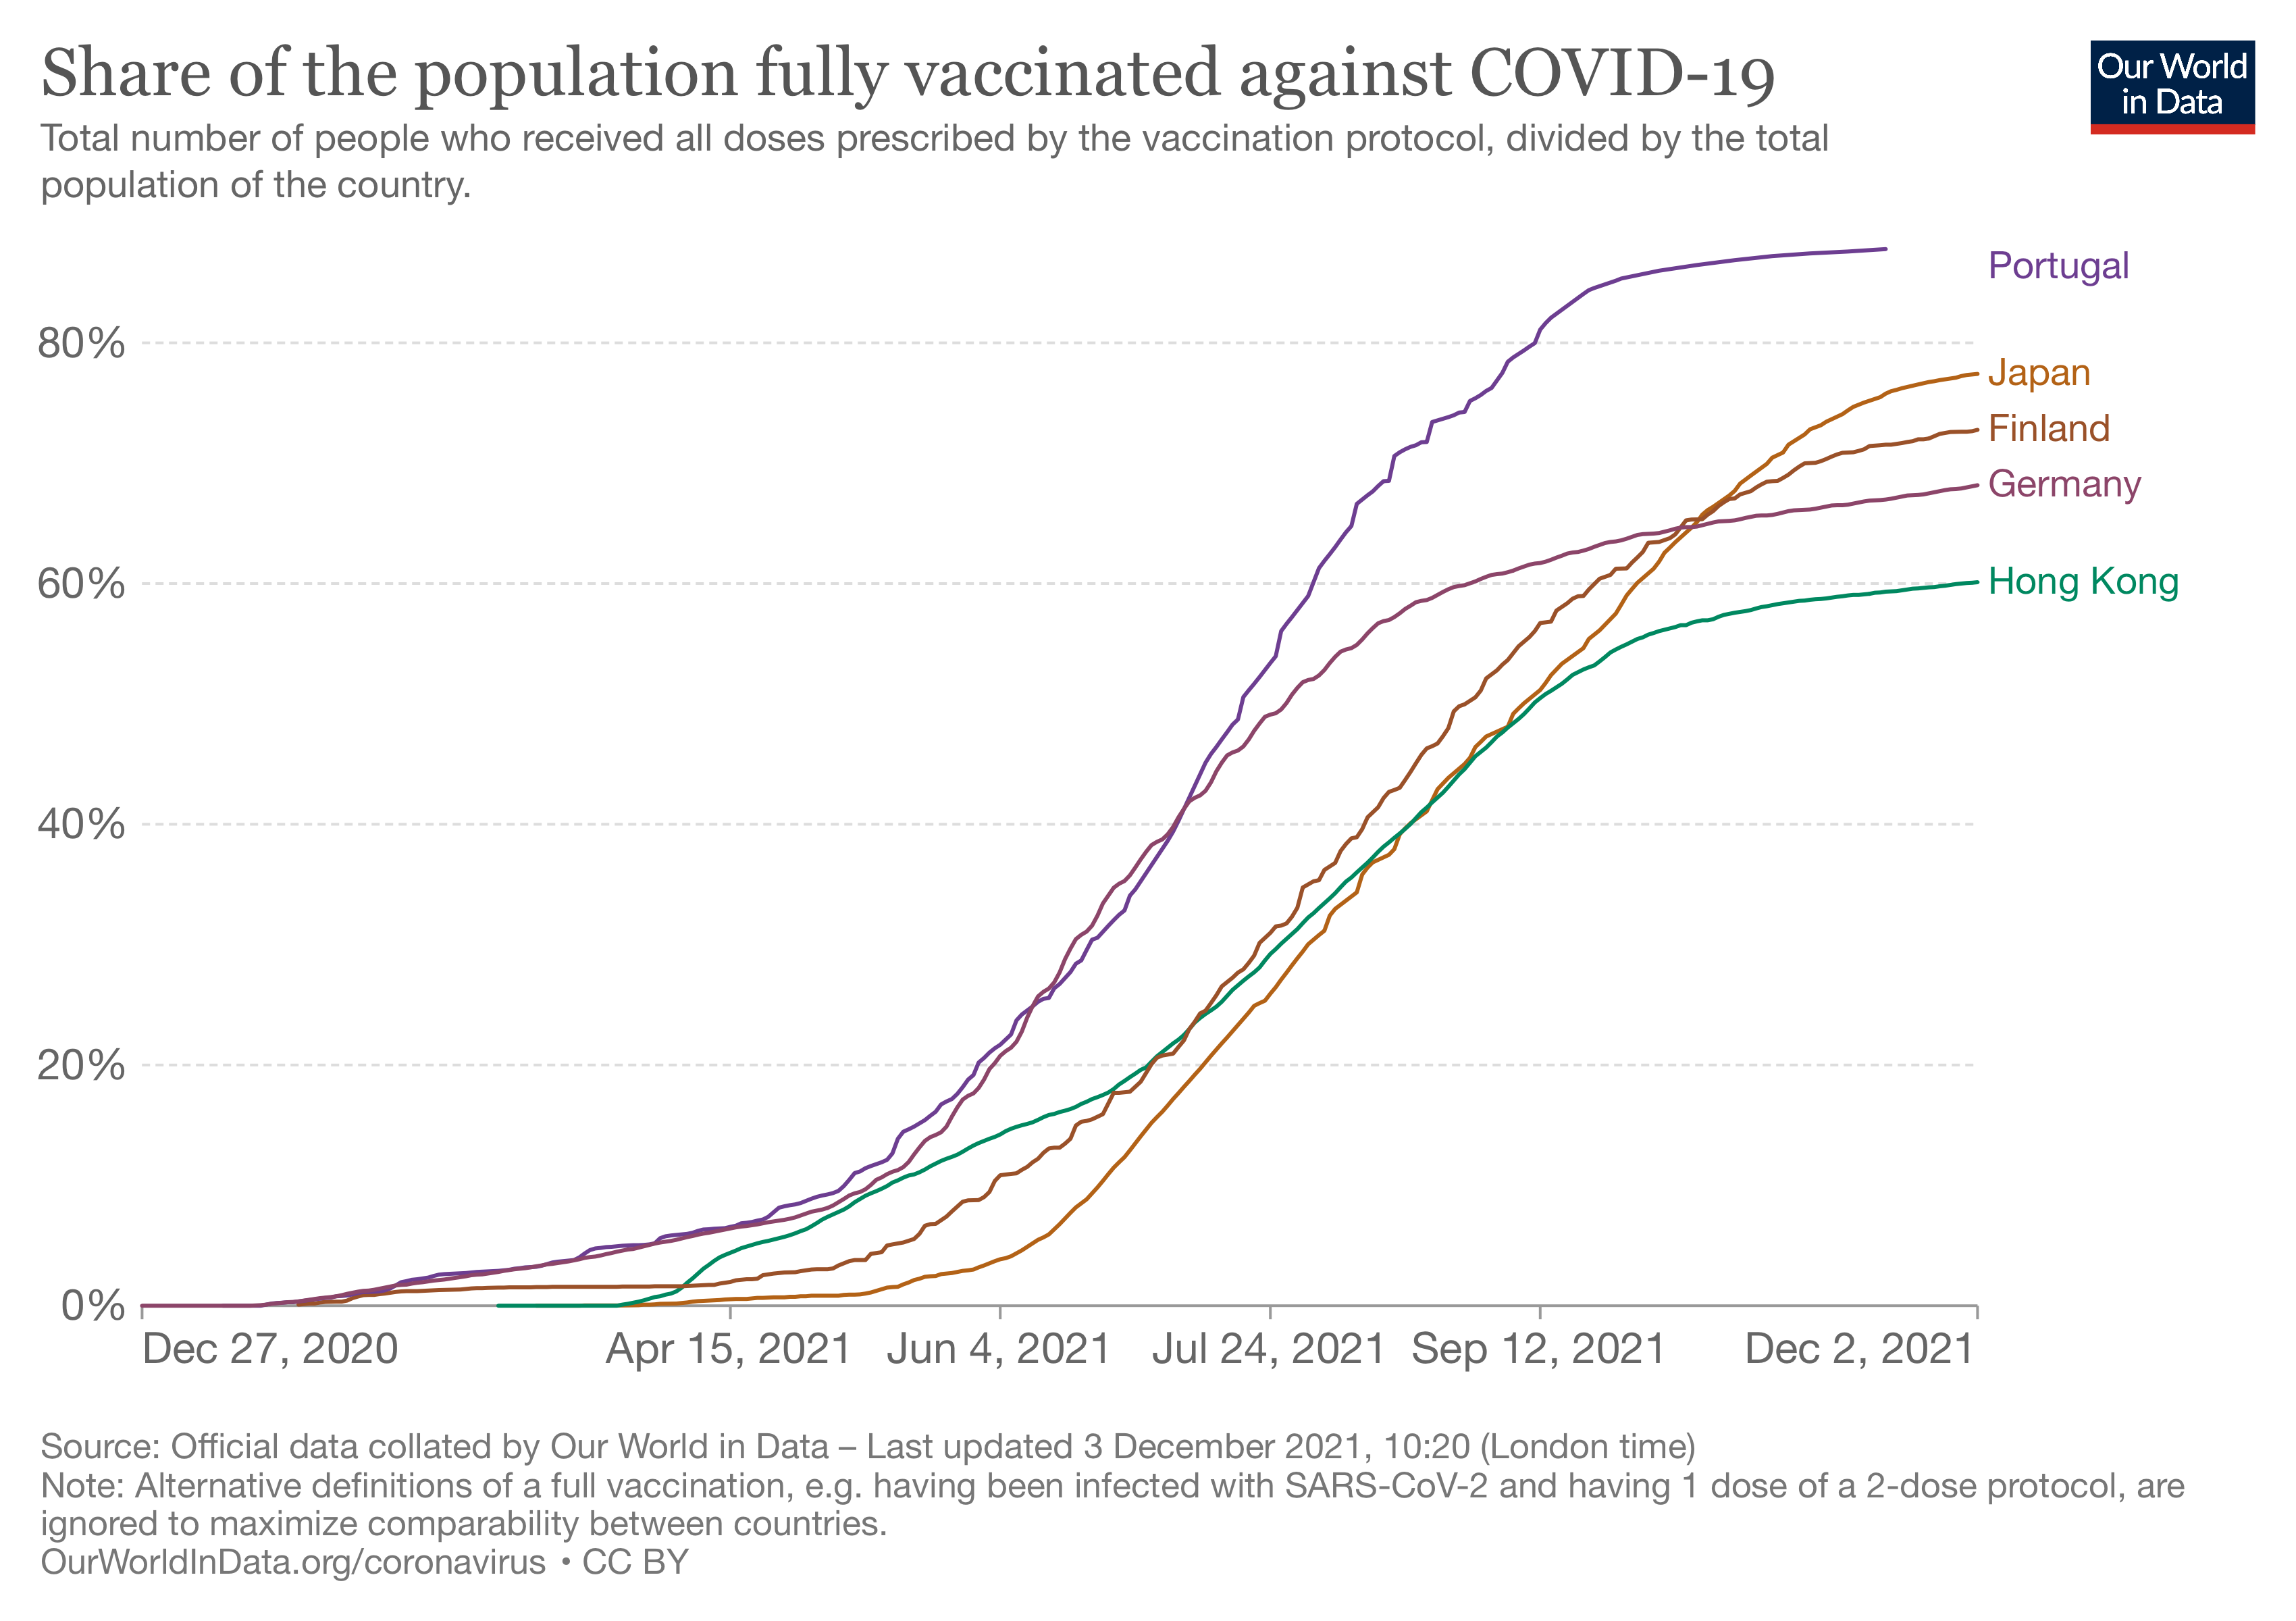
\includegraphics{./image/share-people-fully-vaccinated-covid_plot.png}

\hypertarget{relative-work}{%
\subsubsection{Relative work}\label{relative-work}}

\hypertarget{dataset}{%
\section{2. Dataset}\label{dataset}}

Datasets down below show cumulative covid vaccinations rate by
countries( collected from
\href{https://ourworldindata.org/covid-vaccinations}{linked
phrase}).Country column shows the country of this data. X column is
originally from the date when the country started vaccination to the
recent date of vaccination. We normalized the date column by giving
index 0 to number of date and deviding it with the number of date. As
the time length of the vaccination differs by country, we uniformly
picked the 222 datapoints from the datasets before normalize the X
column. Y column shows the covid vaccination rate in the country. With
the cumulative covid vaccination number, we devide it by 2 times
population because most of the vaccines require 2 doses to be fully
vaccinated. Therefore, dimension of all datasets are (222,3).

\begin{Shaded}
\begin{Highlighting}[]
\CommentTok{\#setwd(\textquotesingle{}/Users/chuhyeongyeong/2021\_period1/bayesian\_data\_analysis/bda\_aalto\_project\textquotesingle{})}
\CommentTok{\#setwd("/home/chooh1/notebooks/BDA/project")}
\NormalTok{finland }\OtherTok{\textless{}{-}} \FunctionTok{read.csv}\NormalTok{(}\StringTok{"data/Finland\_output.csv"}\NormalTok{)}
\NormalTok{germany }\OtherTok{\textless{}{-}} \FunctionTok{read.csv}\NormalTok{(}\StringTok{"data/Germany\_output.csv"}\NormalTok{)}
\NormalTok{hongkong }\OtherTok{\textless{}{-}} \FunctionTok{read.csv}\NormalTok{(}\StringTok{\textquotesingle{}data/Hong Kong\_output.csv\textquotesingle{}}\NormalTok{)}
\NormalTok{portugal }\OtherTok{\textless{}{-}} \FunctionTok{read.csv}\NormalTok{(}\StringTok{\textquotesingle{}data/Portugal\_output.csv\textquotesingle{}}\NormalTok{)}
\NormalTok{japan }\OtherTok{\textless{}{-}} \FunctionTok{read.csv}\NormalTok{(}\StringTok{\textquotesingle{}data/Japan\_output.csv\textquotesingle{}}\NormalTok{)}
\end{Highlighting}
\end{Shaded}

\begin{Shaded}
\begin{Highlighting}[]
\FunctionTok{cat}\NormalTok{(}\StringTok{\textquotesingle{}dimenstion of Finland dataset: \textquotesingle{}}\NormalTok{,}\FunctionTok{dim}\NormalTok{(finland),}\StringTok{\textquotesingle{}}\SpecialCharTok{\textbackslash{}n}\StringTok{\textquotesingle{}}\NormalTok{)}
\end{Highlighting}
\end{Shaded}

\begin{verbatim}
## dimenstion of Finland dataset:  222 3
\end{verbatim}

\begin{Shaded}
\begin{Highlighting}[]
\FunctionTok{cat}\NormalTok{(}\StringTok{\textquotesingle{}dimenstion of Germany dataset: \textquotesingle{}}\NormalTok{,}\FunctionTok{dim}\NormalTok{(germany),}\StringTok{\textquotesingle{}}\SpecialCharTok{\textbackslash{}n}\StringTok{\textquotesingle{}}\NormalTok{)}
\end{Highlighting}
\end{Shaded}

\begin{verbatim}
## dimenstion of Germany dataset:  222 3
\end{verbatim}

\begin{Shaded}
\begin{Highlighting}[]
\FunctionTok{cat}\NormalTok{(}\StringTok{\textquotesingle{}dimenstion of HongKong dataset: \textquotesingle{}}\NormalTok{,}\FunctionTok{dim}\NormalTok{(hongkong),}\StringTok{\textquotesingle{}}\SpecialCharTok{\textbackslash{}n}\StringTok{\textquotesingle{}}\NormalTok{)}
\end{Highlighting}
\end{Shaded}

\begin{verbatim}
## dimenstion of HongKong dataset:  222 3
\end{verbatim}

\begin{Shaded}
\begin{Highlighting}[]
\FunctionTok{cat}\NormalTok{(}\StringTok{\textquotesingle{}dimenstion of Portugal dataset: \textquotesingle{}}\NormalTok{,}\FunctionTok{dim}\NormalTok{(portugal),}\StringTok{\textquotesingle{}}\SpecialCharTok{\textbackslash{}n}\StringTok{\textquotesingle{}}\NormalTok{)}
\end{Highlighting}
\end{Shaded}

\begin{verbatim}
## dimenstion of Portugal dataset:  222 3
\end{verbatim}

\begin{Shaded}
\begin{Highlighting}[]
\FunctionTok{cat}\NormalTok{(}\StringTok{\textquotesingle{}dimenstion of Japan dataset: \textquotesingle{}}\NormalTok{,}\FunctionTok{dim}\NormalTok{(japan),}\StringTok{\textquotesingle{}}\SpecialCharTok{\textbackslash{}n}\StringTok{\textquotesingle{}}\NormalTok{)}
\end{Highlighting}
\end{Shaded}

\begin{verbatim}
## dimenstion of Japan dataset:  222 3
\end{verbatim}

\begin{Shaded}
\begin{Highlighting}[]
\NormalTok{total}\OtherTok{=} \FunctionTok{rbind}\NormalTok{(finland,germany,hongkong,portugal,japan)}
\FunctionTok{ggplot}\NormalTok{(}\AttributeTok{data =}\NormalTok{ total, }\FunctionTok{aes}\NormalTok{(}\AttributeTok{x =}\NormalTok{ X, }\AttributeTok{y =}\NormalTok{ Y, }\AttributeTok{color =}\NormalTok{ Country)) }\SpecialCharTok{+}
    \FunctionTok{geom\_line}\NormalTok{() }\SpecialCharTok{+}
    \FunctionTok{ggtitle}\NormalTok{(}\StringTok{"Cumulative covid19 vaccination rate"}\NormalTok{) }\SpecialCharTok{+}
    \FunctionTok{xlab}\NormalTok{(}\StringTok{"time"}\NormalTok{) }\SpecialCharTok{+} \FunctionTok{ylab}\NormalTok{(}\StringTok{"vaccination rate"}\NormalTok{)}
\end{Highlighting}
\end{Shaded}

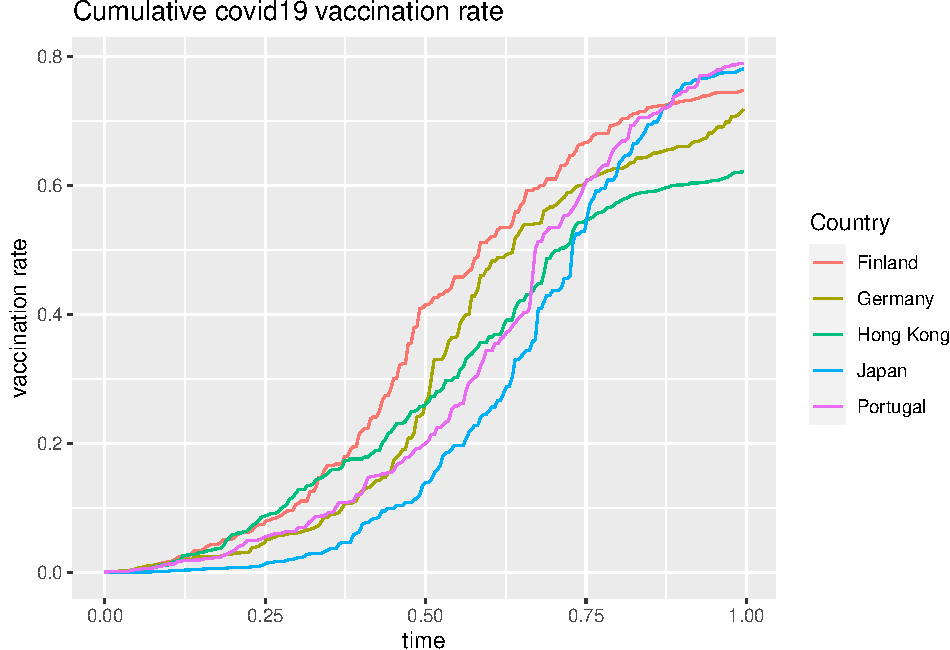
\includegraphics{bda_project_files/figure-latex/unnamed-chunk-7-1.pdf}

\hypertarget{mathematical-models-and-stan-code}{%
\section{3. Mathematical Models and Stan
code}\label{mathematical-models-and-stan-code}}

\hypertarget{seperated-model}{%
\subsection{Seperated Model}\label{seperated-model}}

\[
\begin{aligned}
y_{i j} \mid \mu_i, \sigma &\sim \operatorname{Normal}\left(\mu_i, \sigma\right) \\
\mu_i &\sim \operatorname{logit}(\alpha_i, \beta_i)\\
\sigma &\sim \text{inv}\chi^2(1)\\
\\
\alpha_i &\sim \text{inv}\chi^2(1) \\
\beta_i &\sim N(0.5,1) \\
\end{aligned}
\]

We will first try to build the seperated model in stan

\begin{Shaded}
\begin{Highlighting}[]
\NormalTok{seperated\_model }\OtherTok{\textless{}{-}} \StringTok{"}
\StringTok{functions \{}
\StringTok{  real[] logit\_transform(real[] x, real k, real x0) \{}
\StringTok{    int N = size(x);}
\StringTok{    real xtemp[N];}
\StringTok{    for (i in 1:N)\{}
\StringTok{      xtemp[i] = 1 / (1 + exp({-}k * (x[i] {-} x0)));}
\StringTok{    \}}
\StringTok{     return xtemp;}
\StringTok{  \}}
\StringTok{\}}

\StringTok{data \{}
\StringTok{    int\textless{}lower=0\textgreater{} J;}
\StringTok{    int\textless{}lower=1\textgreater{} M;}
\StringTok{    int\textless{}lower=0\textgreater{} N; // number of data points}
\StringTok{    real x[M,N]; // observation year}
\StringTok{    real y[M,N]; // observation number of drowned}
\StringTok{    real xpred;  // prediction year}
\StringTok{\}}

\StringTok{parameters \{}
\StringTok{  real alpha[M];}
\StringTok{  real beta[M];}
\StringTok{  real\textless{}lower = 0\textgreater{} sigma;}
\StringTok{\}}

\StringTok{transformed parameters \{}
\StringTok{  real mu[M,N];}
\StringTok{  for (i in 1:M)\{}
\StringTok{    mu[i,] = logit\_transform(x[i,],alpha[i], beta[i]);}
\StringTok{  \}}
\StringTok{\}}

\StringTok{model \{}
\StringTok{  for (i in 1:M)\{}
\StringTok{    // as prior we will change it to the same values}
\StringTok{    alpha[i] \textasciitilde{} inv\_chi\_square(1);}
\StringTok{    beta[i] \textasciitilde{} normal(0.5,1);}
\StringTok{  \}}

\StringTok{  sigma \textasciitilde{} inv\_chi\_square(1);}

\StringTok{  //likelihood}
\StringTok{  for (i in 1:M)\{}
\StringTok{    y[i,] \textasciitilde{} normal(mu[i,], sigma);}
\StringTok{  \}}
\StringTok{\}}

\StringTok{generated quantities \{}
\StringTok{  vector[N] log\_lik[M];}
\StringTok{  real ypred[M];}
\StringTok{  real t[1];}
\StringTok{  t[1] = xpred;}
\StringTok{  for (i in 1:M)\{}
\StringTok{    ypred[i] = normal\_rng(logit\_transform(t,alpha[i], beta[i])[1], sigma);}
\StringTok{  \}}

\StringTok{  //log{-}likelihood}
\StringTok{  for (i in 1:M) \{}
\StringTok{    for (j in 1:N) \{}
\StringTok{    log\_lik[i,j] = normal\_lpdf(y[i,j] | mu[i,j], sigma);}
\StringTok{    \}}
\StringTok{  \}}

\StringTok{\}}

\StringTok{"}
\end{Highlighting}
\end{Shaded}

\hypertarget{hirachical-model}{%
\subsection{Hirachical Model}\label{hirachical-model}}

\[
\begin{aligned}
y_{i j} \mid \mu_i, \sigma &\sim \operatorname{Normal}\left(\mu_i, \sigma\right) \\
\mu_i &\sim \operatorname{logit}(\alpha_i, \beta_i)\\
\sigma & \sim \operatorname{Inv}-\chi^{2}(1) \\
\\
\beta_{j}\mid \mu_{\beta}, \sigma_{\beta} &\sim \operatorname{Normal}(\mu_{\beta}, \sigma_{\beta})\\
\alpha_{j} \mid \sigma_{\alpha} & \sim \operatorname{Inv}-\chi^{2}\left(\sigma_{\alpha}\right) \\
\\
\mu_{\beta} & \sim \operatorname{Normal}(0,1)\\
\sigma_{\beta} & \sim \operatorname{Inv}-\chi^{2}(1) \\
\sigma_{\alpha} & \sim \operatorname{Inv}-\chi^{2}(1) \\
\end{aligned}
\]

Now we will build the hierarchical model in stan:

\begin{Shaded}
\begin{Highlighting}[]
\NormalTok{hierarchical\_model }\OtherTok{\textless{}{-}} \StringTok{"}
\StringTok{functions \{}
\StringTok{  real[] logit\_transform(real[] x, real k, real x0) \{}
\StringTok{    int N = size(x);}
\StringTok{    real xtemp[N];}
\StringTok{    for (i in 1:N)\{}
\StringTok{      xtemp[i] = 1 / (1 + exp({-}k * (x[i] {-} x0)));}
\StringTok{    \}}
\StringTok{     return xtemp;}
\StringTok{  \}}
\StringTok{\}}

\StringTok{data \{}
\StringTok{    int\textless{}lower=1\textgreater{} M; //number of country}
\StringTok{    int\textless{}lower=0\textgreater{} N; // number of data points}
\StringTok{    real x[M,N]; //}
\StringTok{    real y[M,N]; //}
\StringTok{    real xpred;  // prediction year}
\StringTok{\}}

\StringTok{parameters \{}
\StringTok{  real alpha[M];}
\StringTok{  real beta[M];}
\StringTok{  real\textless{}lower = 0\textgreater{} sigma;}
\StringTok{  real\textless{}lower = 0\textgreater{} hyper\_sigma;}
\StringTok{  real hyper\_mu;}
\StringTok{  real\textless{}lower = 0\textgreater{} hyper\_alpha;}
\StringTok{\}}

\StringTok{transformed parameters \{}
\StringTok{  real mu[M,N];}
\StringTok{  for (i in 1:M)\{}
\StringTok{    mu[i,] = logit\_transform(x[i,],alpha[i], beta[i]);}
\StringTok{  \}}
\StringTok{\}}

\StringTok{model \{}
\StringTok{    hyper\_mu \textasciitilde{} normal(0, 1);}
\StringTok{    hyper\_sigma \textasciitilde{} inv\_chi\_square(10);}
\StringTok{    hyper\_alpha \textasciitilde{} inv\_chi\_square(10);}

\StringTok{  for (i in 1:M)\{}
\StringTok{    // as prior we will change it to the same values}
\StringTok{    alpha[i] \textasciitilde{} inv\_chi\_square(hyper\_alpha);}
\StringTok{    beta[i] \textasciitilde{} normal(hyper\_mu,hyper\_sigma);}
\StringTok{  \}}

\StringTok{  sigma \textasciitilde{} inv\_chi\_square(1);}

\StringTok{  //likelihood}
\StringTok{  for (i in 1:M)\{}
\StringTok{    y[i,] \textasciitilde{} normal(mu[i,], sigma);}
\StringTok{  \}}
\StringTok{\}}

\StringTok{generated quantities \{}
\StringTok{  vector[N] log\_lik[M];}
\StringTok{  real ypred[M];}
\StringTok{  real t[1];}
\StringTok{  t[1] = xpred;}
\StringTok{  for (i in 1:M)\{}
\StringTok{    ypred[i] = normal\_rng(logit\_transform(t,alpha[i], beta[i])[1], sigma);}
\StringTok{  \}}

\StringTok{  //log{-}likelihood}
\StringTok{  for (i in 1:M) \{}
\StringTok{    for (j in 1:N) \{}
\StringTok{    log\_lik[i,j] = normal\_lpdf(y[i,j] | mu[i,j], sigma);}
\StringTok{    \}}
\StringTok{  \}}

\StringTok{\}}

\StringTok{"}
\end{Highlighting}
\end{Shaded}

\hypertarget{prior-selection}{%
\section{4. Prior selection}\label{prior-selection}}

For both models we choose to use weakly informative priors. We will
first present all prior distribuions in plots, to visualize better their
properties.

\begin{Shaded}
\begin{Highlighting}[]
\NormalTok{x }\OtherTok{\textless{}{-}} \FunctionTok{seq}\NormalTok{(}\AttributeTok{from=}\FloatTok{0.1}\NormalTok{, }\AttributeTok{to=}\DecValTok{5}\NormalTok{, }\AttributeTok{by=}\FloatTok{0.01}\NormalTok{)}
\FunctionTok{plot}\NormalTok{(x, }\FunctionTok{dinvchisq}\NormalTok{(x,}\DecValTok{1}\NormalTok{,}\DecValTok{1}\NormalTok{), }\AttributeTok{ylim=}\FunctionTok{c}\NormalTok{(}\DecValTok{0}\NormalTok{,}\DecValTok{1}\NormalTok{), }\AttributeTok{type=}\StringTok{"l"}\NormalTok{, }\AttributeTok{main=}\StringTok{"inv{-}chi{-}square(1) PDF"}\NormalTok{,}
     \AttributeTok{ylab=}\StringTok{"density"}\NormalTok{, }\AttributeTok{col=}\StringTok{"red"}\NormalTok{)}
\end{Highlighting}
\end{Shaded}

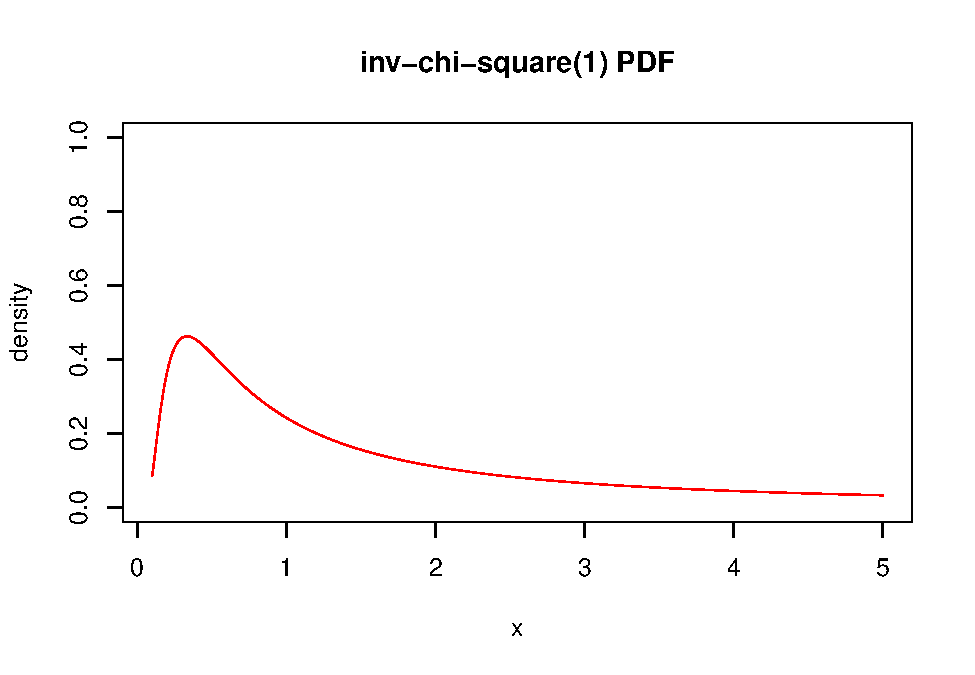
\includegraphics{bda_project_files/figure-latex/unnamed-chunk-10-1.pdf}

\begin{Shaded}
\begin{Highlighting}[]
\NormalTok{x }\OtherTok{\textless{}{-}} \FunctionTok{seq}\NormalTok{(}\AttributeTok{from=}\SpecialCharTok{{-}}\DecValTok{5}\NormalTok{, }\AttributeTok{to=}\DecValTok{5}\NormalTok{, }\AttributeTok{by=}\FloatTok{0.01}\NormalTok{)}
\FunctionTok{plot}\NormalTok{(x, }\FunctionTok{dnorm}\NormalTok{(x, }\FloatTok{0.5}\NormalTok{, }\DecValTok{1}\NormalTok{), }\AttributeTok{ylim=}\FunctionTok{c}\NormalTok{(}\DecValTok{0}\NormalTok{,}\DecValTok{1}\NormalTok{), }\AttributeTok{type=}\StringTok{"l"}\NormalTok{, }\AttributeTok{main=}\StringTok{"Normal(0.5,1) PDF"}\NormalTok{,}
     \AttributeTok{ylab=}\StringTok{"density"}\NormalTok{, }\AttributeTok{col=}\StringTok{"red"}\NormalTok{)}
\end{Highlighting}
\end{Shaded}

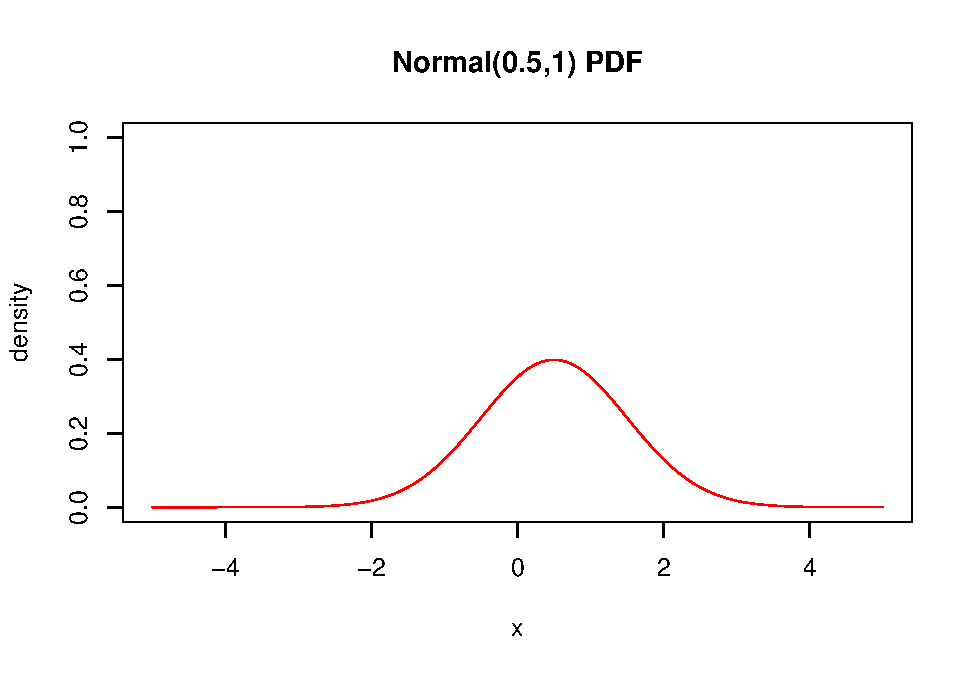
\includegraphics{bda_project_files/figure-latex/unnamed-chunk-11-1.pdf}

\begin{Shaded}
\begin{Highlighting}[]
\NormalTok{x }\OtherTok{\textless{}{-}} \FunctionTok{seq}\NormalTok{(}\AttributeTok{from=}\SpecialCharTok{{-}}\DecValTok{5}\NormalTok{, }\AttributeTok{to=}\DecValTok{5}\NormalTok{, }\AttributeTok{by=}\FloatTok{0.01}\NormalTok{)}
\FunctionTok{plot}\NormalTok{(x, }\FunctionTok{dnorm}\NormalTok{(x, }\DecValTok{0}\NormalTok{, }\DecValTok{1}\NormalTok{), }\AttributeTok{ylim=}\FunctionTok{c}\NormalTok{(}\DecValTok{0}\NormalTok{,}\DecValTok{1}\NormalTok{), }\AttributeTok{type=}\StringTok{"l"}\NormalTok{, }\AttributeTok{main=}\StringTok{"Normal(0,1) PDF"}\NormalTok{,}
     \AttributeTok{ylab=}\StringTok{"density"}\NormalTok{, }\AttributeTok{col=}\StringTok{"red"}\NormalTok{)}
\end{Highlighting}
\end{Shaded}

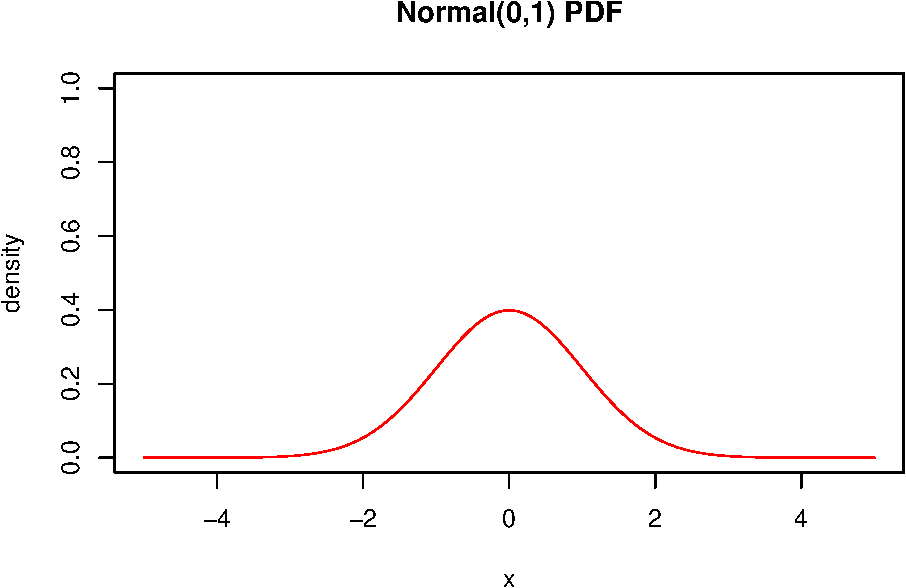
\includegraphics{bda_project_files/figure-latex/unnamed-chunk-12-1.pdf}

\hypertarget{prior-choice-of-the-seperated-model}{%
\subsection{Prior choice of the seperated
model}\label{prior-choice-of-the-seperated-model}}

For the seperated model, the \(\alpha\) prior needed to fullfill two
criteria. First it needed to be a positive number, as we can expect from
the vaccination, that the rate is rising and not dropping. Also, as the
vaccination should follow roughly a logit function, as it can be
observed from the data, we can expect to have a gradient, which is more
likely around \(1\) than bigger than \(50\). Hence the prior of
\(\operatorname{Inv}-\chi^{2}(1)\) was choosen.

For our \(\beta\) prior estimation we know, that it should be in the
range of \([0,1]\), as this is the range of our x-Data. Therefore we
choose \(N(0.5,1)\).

The variance of our y-sampling should be a positive number. As we can
also expect it to be quite small, as we want our model following the
line quite tightly, we choose here as well
\(\operatorname{Inv}-\chi^{2}(1)\).

\hypertarget{prior-choices-of-the-hirachical-model}{%
\subsection{Prior choices of the hirachical
model}\label{prior-choices-of-the-hirachical-model}}

The hirachical model has the following priors. The \(\alpha\)- prior
still has the same distribution function:
\(\operatorname{Inv}-\chi^{2}(\cdot)\), with the same reasoning as for
the seperated model. Here however, the parameter for the function gets
sampled as well. With the same reasoning about the order of magnitude of
our parameter we choose \(\operatorname{Inv}-\chi^{2}(1)\) as a suitable
weakly informative prior. As we can see in the plot above, the PDF of
the probability distribution has nearly all amount of its mass in the
interval of \([0,10]\)

The \(\beta\) prior is again, like in the seperated model a normal
distribution \(N(\cdot,\cdot)\). For the first argument, we choose a
normal distribution of \(N(0,1)\), with the reasoning, that we expect it
to be located somewhere in the interval of \([0,1]\), as this is the
range of the data. The prior of the variance is given by a
\(\operatorname{Inv}-\chi^{2}(1)\), as here as well we want to have a
variance, which is not much larger, than our expected interval.

\hypertarget{stan-code}{%
\section{5. Stan code}\label{stan-code}}

The stan code was provided above with the describtion of the model

\hypertarget{how-to-the-stan-model-was-run-that-is-what-options-were-used.-this-is-also-more-clear-as-combination-of-textual-explanation-and-the-actual-code-line}{%
\section{6. How to the Stan model was run, that is, what options were
used. This is also more clear as combination of textual explanation and
the actual code
line}\label{how-to-the-stan-model-was-run-that-is-what-options-were-used.-this-is-also-more-clear-as-combination-of-textual-explanation-and-the-actual-code-line}}

\begin{Shaded}
\begin{Highlighting}[]
\CommentTok{\# setwd("/Users/max/Documents/UniMac/Aalto/BDA/bda\_aalto\_project/data")}
\CommentTok{\#setwd("/home/chooh1/notebooks/BDA/project")}
\NormalTok{finland }\OtherTok{\textless{}{-}} \FunctionTok{read.csv}\NormalTok{(}\StringTok{"data/Finland\_output.csv"}\NormalTok{)}
\NormalTok{germany }\OtherTok{\textless{}{-}} \FunctionTok{read.csv}\NormalTok{(}\StringTok{"data/Germany\_output.csv"}\NormalTok{)}
\NormalTok{portugal }\OtherTok{\textless{}{-}} \FunctionTok{read.csv}\NormalTok{(}\StringTok{"data/Portugal\_output.csv"}\NormalTok{)}
\NormalTok{hongkong }\OtherTok{\textless{}{-}} \FunctionTok{read.csv}\NormalTok{(}\StringTok{"data/Hong Kong\_output.csv"}\NormalTok{)}
\NormalTok{japan }\OtherTok{\textless{}{-}} \FunctionTok{read.csv}\NormalTok{(}\StringTok{"data/Japan\_output.csv"}\NormalTok{)}
\end{Highlighting}
\end{Shaded}

\begin{Shaded}
\begin{Highlighting}[]
\CommentTok{\#seperate model run}
\NormalTok{xData }\OtherTok{\textless{}{-}} \FunctionTok{rbind}\NormalTok{(finland}\SpecialCharTok{$}\NormalTok{X,germany}\SpecialCharTok{$}\NormalTok{X,portugal}\SpecialCharTok{$}\NormalTok{X,hongkong}\SpecialCharTok{$}\NormalTok{X,japan}\SpecialCharTok{$}\NormalTok{X) }\CommentTok{\#(5,222)}
\NormalTok{yData }\OtherTok{\textless{}{-}}\FunctionTok{rbind}\NormalTok{(finland}\SpecialCharTok{$}\NormalTok{Y,germany}\SpecialCharTok{$}\NormalTok{Y,portugal}\SpecialCharTok{$}\NormalTok{Y,hongkong}\SpecialCharTok{$}\NormalTok{Y,japan}\SpecialCharTok{$}\NormalTok{Y) }\CommentTok{\#(5,222)}

\NormalTok{sm }\OtherTok{\textless{}{-}}\NormalTok{ rstan}\SpecialCharTok{::}\FunctionTok{stan\_model}\NormalTok{(}\AttributeTok{model\_code =}\NormalTok{ seperated\_model)}
\end{Highlighting}
\end{Shaded}

\begin{verbatim}
## Trying to compile a simple C file
\end{verbatim}

\begin{Shaded}
\begin{Highlighting}[]
\NormalTok{stan\_data }\OtherTok{\textless{}{-}} \FunctionTok{list}\NormalTok{(}
    \AttributeTok{J =} \DecValTok{1}\NormalTok{,}
    \AttributeTok{N =} \FunctionTok{dim}\NormalTok{(xData)[}\DecValTok{2}\NormalTok{],}
    \AttributeTok{M =} \FunctionTok{dim}\NormalTok{(xData)[}\DecValTok{1}\NormalTok{],}
    \AttributeTok{y =}\NormalTok{ yData,}
    \AttributeTok{x =}\NormalTok{ xData,}
    \AttributeTok{xpred =} \FloatTok{1.1}
\NormalTok{)}
\NormalTok{model\_separated }\OtherTok{\textless{}{-}}\NormalTok{ rstan}\SpecialCharTok{::}\FunctionTok{sampling}\NormalTok{(sm, }\AttributeTok{data =}\NormalTok{ stan\_data, }\AttributeTok{warmup=}\DecValTok{3000}\NormalTok{, }\AttributeTok{iter=}\DecValTok{4000}\NormalTok{)}
\NormalTok{fit\_sm }\OtherTok{\textless{}{-}} \FunctionTok{extract}\NormalTok{(model\_separated, }\AttributeTok{permuted =} \ConstantTok{TRUE}\NormalTok{, }\AttributeTok{inc\_warmup =} \ConstantTok{FALSE}\NormalTok{)}
\end{Highlighting}
\end{Shaded}

Below graph shows the posterior vaccination rate by countries in
seperate model.

\begin{Shaded}
\begin{Highlighting}[]
\NormalTok{Y\_s }\OtherTok{=} \FunctionTok{c}\NormalTok{(fit\_sm}\SpecialCharTok{$}\NormalTok{mu[}\DecValTok{3000}\NormalTok{,}\DecValTok{1}\NormalTok{,],fit\_sm}\SpecialCharTok{$}\NormalTok{mu[}\DecValTok{3000}\NormalTok{,}\DecValTok{2}\NormalTok{,],fit\_sm}\SpecialCharTok{$}\NormalTok{mu[}\DecValTok{3000}\NormalTok{,}\DecValTok{3}\NormalTok{,],}
\NormalTok{      fit\_sm}\SpecialCharTok{$}\NormalTok{mu[}\DecValTok{3000}\NormalTok{,}\DecValTok{4}\NormalTok{,],fit\_sm}\SpecialCharTok{$}\NormalTok{mu[}\DecValTok{3000}\NormalTok{,}\DecValTok{5}\NormalTok{,])}
\NormalTok{result\_s }\OtherTok{=} \FunctionTok{data.frame}\NormalTok{(}\AttributeTok{Country=}\NormalTok{total}\SpecialCharTok{$}\NormalTok{Country,}\AttributeTok{X=}\NormalTok{total}\SpecialCharTok{$}\NormalTok{X,}\AttributeTok{Y=}\NormalTok{Y\_s)}
\FunctionTok{ggplot}\NormalTok{(}\AttributeTok{data =}\NormalTok{ result\_s, }\FunctionTok{aes}\NormalTok{(}\AttributeTok{x =}\NormalTok{X, }\AttributeTok{y =}\NormalTok{ Y, }\AttributeTok{color =}\NormalTok{ Country)) }\SpecialCharTok{+}
    \FunctionTok{geom\_line}\NormalTok{() }\SpecialCharTok{+}
    \FunctionTok{ggtitle}\NormalTok{(}\StringTok{"Sampled covid19 vaccination rate from the seperated model"}\NormalTok{) }\SpecialCharTok{+}
    \FunctionTok{xlab}\NormalTok{(}\StringTok{"time"}\NormalTok{) }\SpecialCharTok{+} \FunctionTok{ylab}\NormalTok{(}\StringTok{"posterior vaccination rate"}\NormalTok{)}
\end{Highlighting}
\end{Shaded}

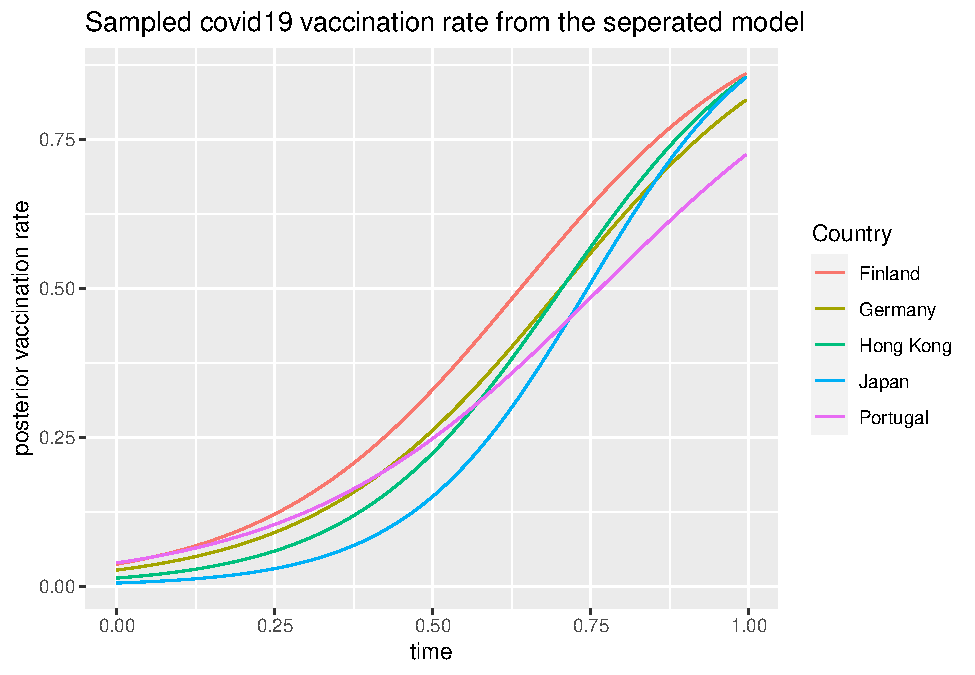
\includegraphics{bda_project_files/figure-latex/unnamed-chunk-15-1.pdf}

\begin{Shaded}
\begin{Highlighting}[]
\CommentTok{\#hierarchical model run}
\NormalTok{hm }\OtherTok{\textless{}{-}}\NormalTok{ rstan}\SpecialCharTok{::}\FunctionTok{stan\_model}\NormalTok{(}\AttributeTok{model\_code =}\NormalTok{ hierarchical\_model)}
\end{Highlighting}
\end{Shaded}

\begin{verbatim}
## Trying to compile a simple C file
\end{verbatim}

\begin{verbatim}
## Running /Library/Frameworks/R.framework/Resources/bin/R CMD SHLIB foo.c
## clang -mmacosx-version-min=10.13 -I"/Library/Frameworks/R.framework/Resources/include" -DNDEBUG   -I"/Library/Frameworks/R.framework/Versions/4.1/Resources/library/Rcpp/include/"  -I"/Library/Frameworks/R.framework/Versions/4.1/Resources/library/RcppEigen/include/"  -I"/Library/Frameworks/R.framework/Versions/4.1/Resources/library/RcppEigen/include/unsupported"  -I"/Library/Frameworks/R.framework/Versions/4.1/Resources/library/BH/include" -I"/Library/Frameworks/R.framework/Versions/4.1/Resources/library/StanHeaders/include/src/"  -I"/Library/Frameworks/R.framework/Versions/4.1/Resources/library/StanHeaders/include/"  -I"/Library/Frameworks/R.framework/Versions/4.1/Resources/library/RcppParallel/include/"  -I"/Library/Frameworks/R.framework/Versions/4.1/Resources/library/rstan/include" -DEIGEN_NO_DEBUG  -DBOOST_DISABLE_ASSERTS  -DBOOST_PENDING_INTEGER_LOG2_HPP  -DSTAN_THREADS  -DBOOST_NO_AUTO_PTR  -include '/Library/Frameworks/R.framework/Versions/4.1/Resources/library/StanHeaders/include/stan/math/prim/mat/fun/Eigen.hpp'  -D_REENTRANT -DRCPP_PARALLEL_USE_TBB=1   -I/usr/local/include   -fPIC  -Wall -g -O2  -c foo.c -o foo.o
## In file included from <built-in>:1:
## In file included from /Library/Frameworks/R.framework/Versions/4.1/Resources/library/StanHeaders/include/stan/math/prim/mat/fun/Eigen.hpp:13:
## In file included from /Library/Frameworks/R.framework/Versions/4.1/Resources/library/RcppEigen/include/Eigen/Dense:1:
## In file included from /Library/Frameworks/R.framework/Versions/4.1/Resources/library/RcppEigen/include/Eigen/Core:88:
## /Library/Frameworks/R.framework/Versions/4.1/Resources/library/RcppEigen/include/Eigen/src/Core/util/Macros.h:628:1: error: unknown type name 'namespace'
## namespace Eigen {
## ^
## /Library/Frameworks/R.framework/Versions/4.1/Resources/library/RcppEigen/include/Eigen/src/Core/util/Macros.h:628:16: error: expected ';' after top level declarator
## namespace Eigen {
##                ^
##                ;
## In file included from <built-in>:1:
## In file included from /Library/Frameworks/R.framework/Versions/4.1/Resources/library/StanHeaders/include/stan/math/prim/mat/fun/Eigen.hpp:13:
## In file included from /Library/Frameworks/R.framework/Versions/4.1/Resources/library/RcppEigen/include/Eigen/Dense:1:
## /Library/Frameworks/R.framework/Versions/4.1/Resources/library/RcppEigen/include/Eigen/Core:96:10: fatal error: 'complex' file not found
## #include <complex>
##          ^~~~~~~~~
## 3 errors generated.
## make: *** [foo.o] Error 1
\end{verbatim}

\begin{Shaded}
\begin{Highlighting}[]
\NormalTok{stan\_data }\OtherTok{\textless{}{-}} \FunctionTok{list}\NormalTok{(}
    \AttributeTok{N =} \FunctionTok{dim}\NormalTok{(xData)[}\DecValTok{2}\NormalTok{],}
    \AttributeTok{M =} \FunctionTok{dim}\NormalTok{(xData)[}\DecValTok{1}\NormalTok{],}
    \AttributeTok{y =}\NormalTok{ yData,}
    \AttributeTok{x =}\NormalTok{ xData,}
    \AttributeTok{xpred =} \FloatTok{1.1}
\NormalTok{)}
\NormalTok{model\_hierarchical }\OtherTok{\textless{}{-}}\NormalTok{ rstan}\SpecialCharTok{::}\FunctionTok{sampling}\NormalTok{(hm, }\AttributeTok{data =}\NormalTok{ stan\_data, }\AttributeTok{warmup=}\DecValTok{3000}\NormalTok{, }\AttributeTok{iter=}\DecValTok{4000}\NormalTok{)}
\end{Highlighting}
\end{Shaded}

\begin{verbatim}
## Warning in .local(object, ...): some chains had errors; consider specifying
## chains = 1 to debug
\end{verbatim}

\begin{verbatim}
## here are whatever error messages were returned
\end{verbatim}

\begin{verbatim}
## [[1]]
## Stan model 'ba8b974ad1b3c178602f6652576f20bb' does not contain samples.
\end{verbatim}

\begin{Shaded}
\begin{Highlighting}[]
\NormalTok{fit\_hm }\OtherTok{\textless{}{-}} \FunctionTok{extract}\NormalTok{(model\_hierarchical, }\AttributeTok{permuted =} \ConstantTok{TRUE}\NormalTok{, }\AttributeTok{inc\_warmup =} \ConstantTok{FALSE}\NormalTok{)}
\end{Highlighting}
\end{Shaded}

Below graph shows the posterior vaccination rate by countries in
hierarchical model.

\begin{Shaded}
\begin{Highlighting}[]
\NormalTok{Y\_h }\OtherTok{=} \FunctionTok{c}\NormalTok{(fit\_hm}\SpecialCharTok{$}\NormalTok{mu[}\DecValTok{3000}\NormalTok{,}\DecValTok{1}\NormalTok{,],fit\_hm}\SpecialCharTok{$}\NormalTok{mu[}\DecValTok{3000}\NormalTok{,}\DecValTok{2}\NormalTok{,],fit\_hm}\SpecialCharTok{$}\NormalTok{mu[}\DecValTok{3000}\NormalTok{,}\DecValTok{3}\NormalTok{,],}
\NormalTok{      fit\_hm}\SpecialCharTok{$}\NormalTok{mu[}\DecValTok{3000}\NormalTok{,}\DecValTok{4}\NormalTok{,],fit\_hm}\SpecialCharTok{$}\NormalTok{mu[}\DecValTok{3000}\NormalTok{,}\DecValTok{5}\NormalTok{,])}
\NormalTok{result\_h }\OtherTok{=} \FunctionTok{data.frame}\NormalTok{(}\AttributeTok{Country=}\NormalTok{total}\SpecialCharTok{$}\NormalTok{Country,}\AttributeTok{X=}\NormalTok{total}\SpecialCharTok{$}\NormalTok{X,}\AttributeTok{Y=}\NormalTok{Y\_h)}
\FunctionTok{ggplot}\NormalTok{(}\AttributeTok{data =}\NormalTok{ result\_h, }\FunctionTok{aes}\NormalTok{(}\AttributeTok{x =}\NormalTok{X, }\AttributeTok{y =}\NormalTok{ Y, }\AttributeTok{color =}\NormalTok{ Country)) }\SpecialCharTok{+}
    \FunctionTok{geom\_line}\NormalTok{() }\SpecialCharTok{+}
    \FunctionTok{ggtitle}\NormalTok{(}\StringTok{"Sampled covid19 vaccination rate from the hierarchical model"}\NormalTok{) }\SpecialCharTok{+}
    \FunctionTok{xlab}\NormalTok{(}\StringTok{"time"}\NormalTok{) }\SpecialCharTok{+} \FunctionTok{ylab}\NormalTok{(}\StringTok{"posterior vaccination rate"}\NormalTok{)}
\end{Highlighting}
\end{Shaded}

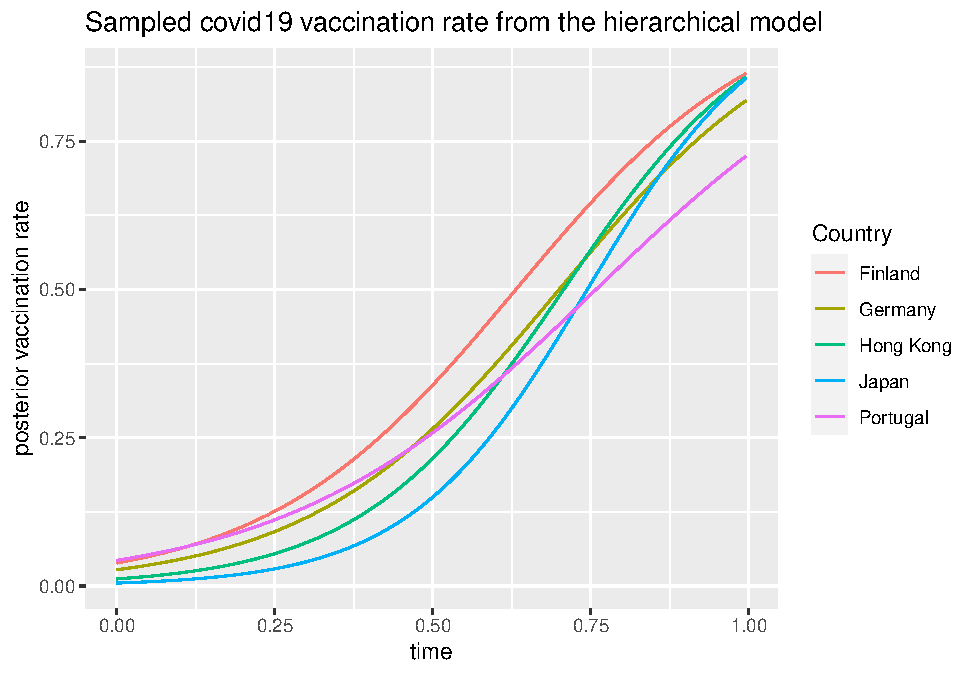
\includegraphics{bda_project_files/figure-latex/unnamed-chunk-17-1.pdf}

With the command \texttt{rstan::stan\_model} we compile our stan models
from a string vector and in the next step with \texttt{rstan::sampling}
we create samples from the models. The given data are the datasets from
section 2. As a warmup phase we use the generous length of \(3000\) and
as a total chain length \(4000\). As the warmup lenght is longer than
half of the chain length we made sure, that the samples are within our
posterior distribution.

\hypertarget{convergence-diagnostics-rhat-ess-divergences-and-what-was-done-if-the-convergence-was-not-good-with-the-first-try.}{%
\section{7.Convergence diagnostics (Rhat, ESS, divergences) and what was
done if the convergence was not good with the first
try.}\label{convergence-diagnostics-rhat-ess-divergences-and-what-was-done-if-the-convergence-was-not-good-with-the-first-try.}}

We will use the build in tool from the stan library to analyse the
convergence of our chains.

\begin{Shaded}
\begin{Highlighting}[]
\CommentTok{\#seperate model}
\NormalTok{sum\_seperate }\OtherTok{\textless{}{-}} \FunctionTok{summary}\NormalTok{(model\_separated)}
\FunctionTok{cat}\NormalTok{(}\StringTok{"Rhat of seperate model: }\SpecialCharTok{\textbackslash{}n}\StringTok{"}\NormalTok{)}
\end{Highlighting}
\end{Shaded}

\begin{verbatim}
## Rhat of seperate model:
\end{verbatim}

\begin{Shaded}
\begin{Highlighting}[]
\NormalTok{sum\_seperate}\SpecialCharTok{$}\NormalTok{summary[}\DecValTok{1}\SpecialCharTok{:}\DecValTok{11}\NormalTok{,}\DecValTok{10}\NormalTok{]}
\end{Highlighting}
\end{Shaded}

\begin{verbatim}
##  alpha[1]  alpha[2]  alpha[3]  alpha[4]  alpha[5]   beta[1]   beta[2]   beta[3] 
## 0.9995340 0.9995751 0.9996820 0.9997284 0.9995422 0.9992815 0.9993272 0.9996538 
##   beta[4]   beta[5]     sigma 
## 0.9999397 0.9996344 1.0002881
\end{verbatim}

\begin{Shaded}
\begin{Highlighting}[]
\CommentTok{\#hierarchical}
\NormalTok{sum\_hierarchical }\OtherTok{\textless{}{-}} \FunctionTok{summary}\NormalTok{(model\_hierarchical)}
\FunctionTok{cat}\NormalTok{(}\StringTok{"Rhat of hierarchical model: }\SpecialCharTok{\textbackslash{}n}\StringTok{"}\NormalTok{)}
\end{Highlighting}
\end{Shaded}

\begin{verbatim}
## Rhat of hierarchical model:
\end{verbatim}

\begin{Shaded}
\begin{Highlighting}[]
\NormalTok{sum\_hierarchical}\SpecialCharTok{$}\NormalTok{summary[}\DecValTok{1}\SpecialCharTok{:}\DecValTok{11}\NormalTok{,}\DecValTok{10}\NormalTok{]}
\end{Highlighting}
\end{Shaded}

\begin{verbatim}
##  alpha[1]  alpha[2]  alpha[3]  alpha[4]  alpha[5]   beta[1]   beta[2]   beta[3] 
## 0.9993076 0.9996798 0.9991663 1.0001276 0.9994699 0.9995941 0.9996060 0.9994629 
##   beta[4]   beta[5]     sigma 
## 0.9997711 0.9995995 0.9994361
\end{verbatim}

\[
\begin{aligned}
\hat{R} = \sqrt\frac{\hat{var^*}}{W}
\end{aligned}
\]

R hat is potential scale reduction factor. This value estimates how much
the scale could reduce if N goes infinite. When N approches infinity, R
hat approches 1. If R hat is bigger than 1.01, we should keep sampling.

As we can see here, the \(\hat{R}\) values are less than 1, which means,
that the chains converges. We will now run the ESS analysis, to further
verify, that our \(\hat{R}\) values are trustworthy. As mentioned in
Verteri et al.~2019, a ESS value above 400 will indicate that the
\(\hat{R}\) value is reliable. We therefore now use the ESS method from
Verteri et al.~2019:

\begin{Shaded}
\begin{Highlighting}[]
\FunctionTok{cat}\NormalTok{(}\StringTok{"ESS of seperated model: }\SpecialCharTok{\textbackslash{}n}\StringTok{"}\NormalTok{)}
\end{Highlighting}
\end{Shaded}

\begin{verbatim}
## ESS of seperated model:
\end{verbatim}

\begin{Shaded}
\begin{Highlighting}[]
\NormalTok{sum\_seperate}\SpecialCharTok{$}\NormalTok{summary[}\DecValTok{1}\SpecialCharTok{:}\DecValTok{11}\NormalTok{,}\DecValTok{9}\NormalTok{]}
\end{Highlighting}
\end{Shaded}

\begin{verbatim}
## alpha[1] alpha[2] alpha[3] alpha[4] alpha[5]  beta[1]  beta[2]  beta[3] 
## 6457.006 7679.095 7622.422 6490.886 7607.958 7441.946 6800.970 7509.966 
##  beta[4]  beta[5]    sigma 
## 5675.801 7507.722 8418.129
\end{verbatim}

\begin{Shaded}
\begin{Highlighting}[]
\FunctionTok{cat}\NormalTok{(}\StringTok{"ESS of hiracical model: }\SpecialCharTok{\textbackslash{}n}\StringTok{"}\NormalTok{)}
\end{Highlighting}
\end{Shaded}

\begin{verbatim}
## ESS of hiracical model:
\end{verbatim}

\begin{Shaded}
\begin{Highlighting}[]
\NormalTok{sum\_hierarchical}\SpecialCharTok{$}\NormalTok{summary[}\DecValTok{1}\SpecialCharTok{:}\DecValTok{11}\NormalTok{,}\DecValTok{9}\NormalTok{]}
\end{Highlighting}
\end{Shaded}

\begin{verbatim}
## alpha[1] alpha[2] alpha[3] alpha[4] alpha[5]  beta[1]  beta[2]  beta[3] 
## 5292.515 5144.994 5305.628 5252.085 5323.966 4762.507 6349.832 6009.586 
##  beta[4]  beta[5]    sigma 
## 4517.837 5520.833 5228.068
\end{verbatim}

Here we can nicely see, that all ESS values are above 400, which
indicates, that our \(\hat{R}\) values are realiable. We can therefore
conclude, that our chains converged.

\hypertarget{posterior-predictive-checks-and-what-was-done-to-improve-the-model.}{%
\section{8. Posterior predictive checks and what was done to improve the
model.}\label{posterior-predictive-checks-and-what-was-done-to-improve-the-model.}}

\begin{Shaded}
\begin{Highlighting}[]
\CommentTok{\#the posterior expectation for parameter with a 90\% credible interval}
\NormalTok{mu\_pred\_interval}\OtherTok{\textless{}{-}}\ControlFlowTok{function}\NormalTok{(data, prob)\{}
\NormalTok{degree }\OtherTok{=} \FunctionTok{length}\NormalTok{(data)}\SpecialCharTok{{-}}\DecValTok{1}
\NormalTok{mu }\OtherTok{=} \FunctionTok{mean}\NormalTok{(data)}
\NormalTok{sig }\OtherTok{=} \FunctionTok{sqrt}\NormalTok{(}\FunctionTok{var}\NormalTok{(data)}\SpecialCharTok{*}\NormalTok{(}\DecValTok{1}\SpecialCharTok{+}\DecValTok{1}\SpecialCharTok{/}\FunctionTok{length}\NormalTok{(data)))}
\NormalTok{error }\OtherTok{=} \FunctionTok{qt}\NormalTok{(prob}\SpecialCharTok{+}\NormalTok{(}\DecValTok{1}\SpecialCharTok{{-}}\NormalTok{prob)}\SpecialCharTok{/}\DecValTok{2}\NormalTok{,degree)}\SpecialCharTok{*}\NormalTok{sig}
\NormalTok{lower }\OtherTok{=}\NormalTok{ mu }\SpecialCharTok{{-}}\NormalTok{error}
\NormalTok{upper }\OtherTok{=}\NormalTok{ mu }\SpecialCharTok{+}\NormalTok{error}
\NormalTok{interval }\OtherTok{=} \FunctionTok{c}\NormalTok{(lower,upper)}
\FunctionTok{return}\NormalTok{(interval)}
\NormalTok{\}}
\end{Highlighting}
\end{Shaded}

\hypertarget{seperate-model}{%
\subsection{Seperate model}\label{seperate-model}}

\hypertarget{the-posterior-expectations-for-alpha-with-a-90-credible-interval}{%
\subsubsection{The posterior expectations for alpha with a 90\% credible
interval}\label{the-posterior-expectations-for-alpha-with-a-90-credible-interval}}

\begin{Shaded}
\begin{Highlighting}[]
\NormalTok{a1 }\OtherTok{=} \FunctionTok{mu\_pred\_interval}\NormalTok{(}\AttributeTok{data =}\NormalTok{ fit\_sm}\SpecialCharTok{$}\NormalTok{alpha[,}\DecValTok{1}\NormalTok{], }\AttributeTok{prob =} \FloatTok{0.90}\NormalTok{)}
\NormalTok{a2 }\OtherTok{=} \FunctionTok{mu\_pred\_interval}\NormalTok{(}\AttributeTok{data =}\NormalTok{ fit\_sm}\SpecialCharTok{$}\NormalTok{alpha[,}\DecValTok{2}\NormalTok{], }\AttributeTok{prob =} \FloatTok{0.90}\NormalTok{)}
\NormalTok{a3 }\OtherTok{=} \FunctionTok{mu\_pred\_interval}\NormalTok{(}\AttributeTok{data =}\NormalTok{ fit\_sm}\SpecialCharTok{$}\NormalTok{alpha[,}\DecValTok{3}\NormalTok{], }\AttributeTok{prob =} \FloatTok{0.90}\NormalTok{)}
\NormalTok{a4 }\OtherTok{=} \FunctionTok{mu\_pred\_interval}\NormalTok{(}\AttributeTok{data =}\NormalTok{ fit\_sm}\SpecialCharTok{$}\NormalTok{alpha[,}\DecValTok{4}\NormalTok{], }\AttributeTok{prob =} \FloatTok{0.90}\NormalTok{)}
\NormalTok{a5 }\OtherTok{=} \FunctionTok{mu\_pred\_interval}\NormalTok{(}\AttributeTok{data =}\NormalTok{ fit\_sm}\SpecialCharTok{$}\NormalTok{alpha[,}\DecValTok{5}\NormalTok{], }\AttributeTok{prob =} \FloatTok{0.90}\NormalTok{)}
\FunctionTok{cat}\NormalTok{()}
\FunctionTok{cat}\NormalTok{()}
\end{Highlighting}
\end{Shaded}

\hypertarget{the-posterior-expectation-for-betas-with-a-90-credible-interval}{%
\subsubsection{the posterior expectation for betas with a 90\% credible
interval}\label{the-posterior-expectation-for-betas-with-a-90-credible-interval}}

\begin{Shaded}
\begin{Highlighting}[]
\NormalTok{b1 }\OtherTok{=} \FunctionTok{mu\_pred\_interval}\NormalTok{(}\AttributeTok{data =}\NormalTok{ fit\_sm}\SpecialCharTok{$}\NormalTok{beta[,}\DecValTok{1}\NormalTok{], }\AttributeTok{prob =} \FloatTok{0.90}\NormalTok{)}
\NormalTok{b2 }\OtherTok{=} \FunctionTok{mu\_pred\_interval}\NormalTok{(}\AttributeTok{data =}\NormalTok{ fit\_sm}\SpecialCharTok{$}\NormalTok{beta[,}\DecValTok{2}\NormalTok{], }\AttributeTok{prob =} \FloatTok{0.90}\NormalTok{)}
\NormalTok{b3 }\OtherTok{=} \FunctionTok{mu\_pred\_interval}\NormalTok{(}\AttributeTok{data =}\NormalTok{ fit\_sm}\SpecialCharTok{$}\NormalTok{beta[,}\DecValTok{3}\NormalTok{], }\AttributeTok{prob =} \FloatTok{0.90}\NormalTok{)}
\NormalTok{b4 }\OtherTok{=} \FunctionTok{mu\_pred\_interval}\NormalTok{(}\AttributeTok{data =}\NormalTok{ fit\_sm}\SpecialCharTok{$}\NormalTok{beta[,}\DecValTok{4}\NormalTok{], }\AttributeTok{prob =} \FloatTok{0.90}\NormalTok{)}
\NormalTok{b5 }\OtherTok{=} \FunctionTok{mu\_pred\_interval}\NormalTok{(}\AttributeTok{data =}\NormalTok{ fit\_sm}\SpecialCharTok{$}\NormalTok{beta[,}\DecValTok{5}\NormalTok{], }\AttributeTok{prob =} \FloatTok{0.90}\NormalTok{)}
\end{Highlighting}
\end{Shaded}

\hypertarget{model-comparison-e.g.-with-loo-cv}{%
\section{9.Model comparison (e.g.~with
LOO-CV)}\label{model-comparison-e.g.-with-loo-cv}}

\begin{Shaded}
\begin{Highlighting}[]
\CommentTok{\#seperate model extract log\_lik}
\NormalTok{l\_like\_s }\OtherTok{\textless{}{-}} \FunctionTok{extract\_log\_lik}\NormalTok{(model\_separated)}
\NormalTok{loo\_s }\OtherTok{\textless{}{-}} \FunctionTok{loo}\NormalTok{(l\_like\_s)}
\end{Highlighting}
\end{Shaded}

\begin{verbatim}
## Warning: Relative effective sample sizes ('r_eff' argument) not specified.
## For models fit with MCMC, the reported PSIS effective sample sizes and 
## MCSE estimates will be over-optimistic.
\end{verbatim}

\begin{Shaded}
\begin{Highlighting}[]
\NormalTok{elpd\_s }\OtherTok{\textless{}{-}}\NormalTok{ loo\_s}\SpecialCharTok{$}\NormalTok{estimates[}\DecValTok{1}\NormalTok{,}\DecValTok{1}\NormalTok{]}

\CommentTok{\#hierarchical model extract log\_lik}
\NormalTok{l\_like\_h }\OtherTok{\textless{}{-}} \FunctionTok{extract\_log\_lik}\NormalTok{(model\_hierarchical)}
\NormalTok{loo\_h }\OtherTok{\textless{}{-}} \FunctionTok{loo}\NormalTok{(l\_like\_h)}
\end{Highlighting}
\end{Shaded}

\begin{verbatim}
## Warning: Relative effective sample sizes ('r_eff' argument) not specified.
## For models fit with MCMC, the reported PSIS effective sample sizes and 
## MCSE estimates will be over-optimistic.
\end{verbatim}

\begin{Shaded}
\begin{Highlighting}[]
\NormalTok{elpd\_h }\OtherTok{\textless{}{-}}\NormalTok{ loo\_h}\SpecialCharTok{$}\NormalTok{estimates[}\DecValTok{1}\NormalTok{,}\DecValTok{1}\NormalTok{]}
\end{Highlighting}
\end{Shaded}

\begin{Shaded}
\begin{Highlighting}[]
\NormalTok{k\_s }\OtherTok{\textless{}{-}}\NormalTok{ loo\_s}\SpecialCharTok{$}\NormalTok{diagnostics}\SpecialCharTok{$}\NormalTok{pareto\_k}
\NormalTok{plot\_s }\OtherTok{\textless{}{-}} \FunctionTok{ggplot}\NormalTok{(}\AttributeTok{data =} \FunctionTok{data.frame}\NormalTok{(}\AttributeTok{x =} \FunctionTok{seq}\NormalTok{(}\DecValTok{1}\NormalTok{,}\FunctionTok{length}\NormalTok{(k\_s)) ,}\AttributeTok{y =}\NormalTok{ k\_s))}
\NormalTok{plot\_s }\SpecialCharTok{+} \FunctionTok{geom\_point}\NormalTok{(}\FunctionTok{aes}\NormalTok{(}\AttributeTok{x =}\NormalTok{ x, }\AttributeTok{y =}\NormalTok{ y, }\AttributeTok{color =} \StringTok{"blue"}\NormalTok{), }\AttributeTok{alpha =} \FloatTok{0.8}\NormalTok{) }\SpecialCharTok{+}
    \FunctionTok{theme\_light}\NormalTok{() }\SpecialCharTok{+}
    \FunctionTok{xlab}\NormalTok{(}\StringTok{""}\NormalTok{) }\SpecialCharTok{+}
    \FunctionTok{ylab}\NormalTok{(}\StringTok{"k{-}value"}\NormalTok{) }\SpecialCharTok{+}
    \FunctionTok{theme}\NormalTok{(}\AttributeTok{legend.position=}\StringTok{"none"}\NormalTok{)}\SpecialCharTok{+}
    \FunctionTok{ggtitle}\NormalTok{(}\StringTok{"K{-}values in seperate model"}\NormalTok{)}
\end{Highlighting}
\end{Shaded}

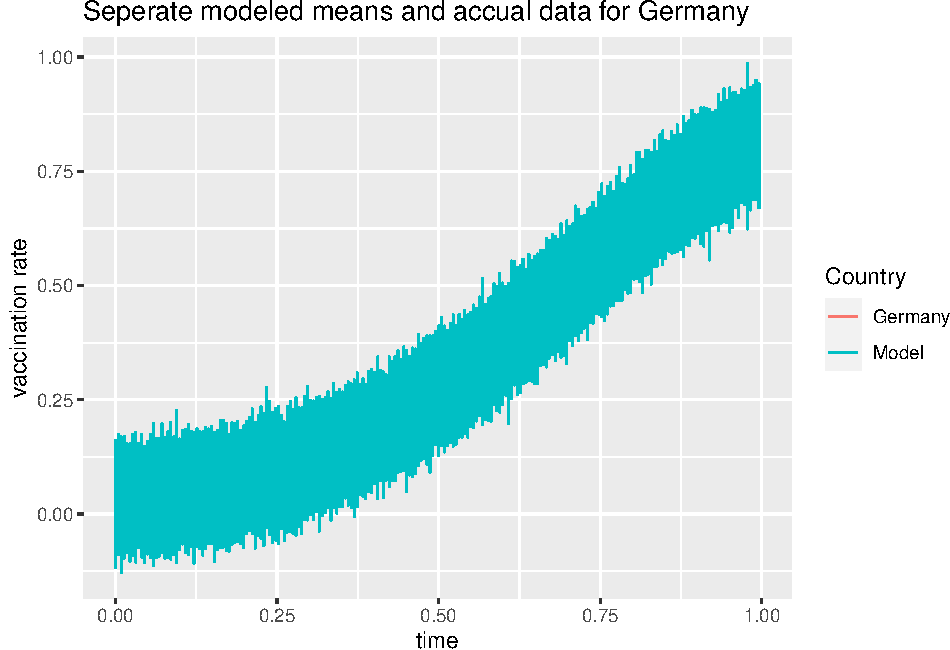
\includegraphics{bda_project_files/figure-latex/unnamed-chunk-26-1.pdf}

\begin{Shaded}
\begin{Highlighting}[]
\NormalTok{k\_h }\OtherTok{\textless{}{-}}\NormalTok{ loo\_h}\SpecialCharTok{$}\NormalTok{diagnostics}\SpecialCharTok{$}\NormalTok{pareto\_k}
\NormalTok{plot\_h }\OtherTok{\textless{}{-}} \FunctionTok{ggplot}\NormalTok{(}\AttributeTok{data =} \FunctionTok{data.frame}\NormalTok{(}\AttributeTok{x =} \FunctionTok{seq}\NormalTok{(}\DecValTok{1}\NormalTok{,}\FunctionTok{length}\NormalTok{(k\_h)) ,}\AttributeTok{y =}\NormalTok{ k\_h))}
\NormalTok{plot\_h }\SpecialCharTok{+} \FunctionTok{geom\_point}\NormalTok{(}\FunctionTok{aes}\NormalTok{(}\AttributeTok{x =}\NormalTok{ x, }\AttributeTok{y =}\NormalTok{ y, }\AttributeTok{color =} \StringTok{"blue"}\NormalTok{), }\AttributeTok{alpha =} \FloatTok{0.8}\NormalTok{) }\SpecialCharTok{+}
    \FunctionTok{theme\_light}\NormalTok{() }\SpecialCharTok{+}
    \FunctionTok{xlab}\NormalTok{(}\StringTok{""}\NormalTok{) }\SpecialCharTok{+}
    \FunctionTok{ylab}\NormalTok{(}\StringTok{"k{-}value"}\NormalTok{) }\SpecialCharTok{+}
    \FunctionTok{theme}\NormalTok{(}\AttributeTok{legend.position=}\StringTok{"none"}\NormalTok{)}\SpecialCharTok{+}
    \FunctionTok{ggtitle}\NormalTok{(}\StringTok{"K{-}values in hierarchical model"}\NormalTok{)}
\end{Highlighting}
\end{Shaded}

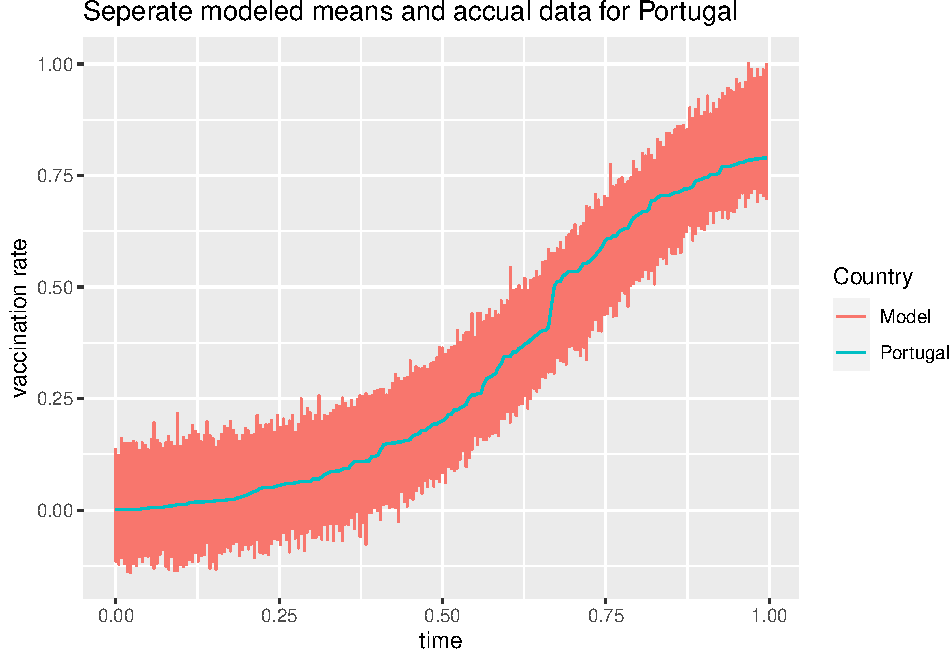
\includegraphics{bda_project_files/figure-latex/unnamed-chunk-27-1.pdf}

\begin{Shaded}
\begin{Highlighting}[]
\FunctionTok{cat}\NormalTok{(}\StringTok{"Maximum k{-}values in seperate model is "}\NormalTok{,}\FunctionTok{max}\NormalTok{(k\_s),}\StringTok{\textquotesingle{}}\SpecialCharTok{\textbackslash{}n}\StringTok{\textquotesingle{}}\NormalTok{)}
\end{Highlighting}
\end{Shaded}

\begin{verbatim}
## Maximum k-values in seperate model is  0.2712977
\end{verbatim}

\begin{Shaded}
\begin{Highlighting}[]
\FunctionTok{cat}\NormalTok{(}\StringTok{"Maximum k{-}values in hierarchical model is "}\NormalTok{,}\FunctionTok{max}\NormalTok{(k\_h),}\StringTok{\textquotesingle{}}\SpecialCharTok{\textbackslash{}n}\StringTok{\textquotesingle{}}\NormalTok{)}
\end{Highlighting}
\end{Shaded}

\begin{verbatim}
## Maximum k-values in hierarchical model is  0.230005
\end{verbatim}

If the k \textless{} 0.7 we can say that PSIS-LOO estimates are
reliable. Based on this,for seperate model and hierarchical model both,
the \hat{k}-values are all below 0.5 which are good. Therefore, both
seperate model and hierarchicalmodels are reliable. However, the maximum
\hat{k}-values in seperate model is 0.216 and the maximum \hat{k}-values
in hierarchical model is 0.176, so we could say the hierarchical model
is more reliable.

\#\#\#\#comparing PSIS-LOO estimates

\begin{Shaded}
\begin{Highlighting}[]
\FunctionTok{cat}\NormalTok{(}\StringTok{"PSIS{-}LOO estimates in seperate model"}\NormalTok{,elpd\_s,}\StringTok{\textquotesingle{}}\SpecialCharTok{\textbackslash{}n}\StringTok{\textquotesingle{}}\NormalTok{)}
\end{Highlighting}
\end{Shaded}

\begin{verbatim}
## PSIS-LOO estimates in seperate model 1958.829
\end{verbatim}

\begin{Shaded}
\begin{Highlighting}[]
\FunctionTok{cat}\NormalTok{(}\StringTok{"PSIS{-}LOO estimates in hierarchical model"}\NormalTok{,elpd\_h,}\StringTok{\textquotesingle{}}\SpecialCharTok{\textbackslash{}n}\StringTok{\textquotesingle{}}\NormalTok{)}
\end{Highlighting}
\end{Shaded}

\begin{verbatim}
## PSIS-LOO estimates in hierarchical model 1958.896
\end{verbatim}

According to the PSIS-LOO estimate, hierarchical model has slightly
higher value for the PSIS-LOO estimate than seperate model,so we could
choose hierarchical model but still seperate model also have nice score
in PSIS-LOO estimate.

\hypertarget{predictive-performance-assessment-if-applicable-e.g.-classification-accuracy-and-evaluation-of-practical-usefulness-of-the-accuracy}{%
\section{10. Predictive performance assessment if applicable
(e.g.~classification accuracy) and evaluation of practical usefulness of
the
accuracy}\label{predictive-performance-assessment-if-applicable-e.g.-classification-accuracy-and-evaluation-of-practical-usefulness-of-the-accuracy}}

We can now evaluate the predictive performance of our model.

\hypertarget{seperate-model-1}{%
\subsection{Seperate model}\label{seperate-model-1}}

For the seperated model we have the following numbers:

\begin{Shaded}
\begin{Highlighting}[]
\FunctionTok{qplot}\NormalTok{(fit\_sm}\SpecialCharTok{$}\NormalTok{ypred[,}\DecValTok{1}\NormalTok{], }\AttributeTok{geom=}\StringTok{"histogram"}\NormalTok{) }\SpecialCharTok{+}
    \FunctionTok{xlab}\NormalTok{(}\StringTok{""}\NormalTok{) }\SpecialCharTok{+}
    \FunctionTok{ylab}\NormalTok{(}\StringTok{""}\NormalTok{) }\SpecialCharTok{+}
    \FunctionTok{ggtitle}\NormalTok{(}\StringTok{"Prediction of vaccination rate in close future,Finland"}\NormalTok{)}
\end{Highlighting}
\end{Shaded}

\begin{verbatim}
## `stat_bin()` using `bins = 30`. Pick better value with `binwidth`.
\end{verbatim}

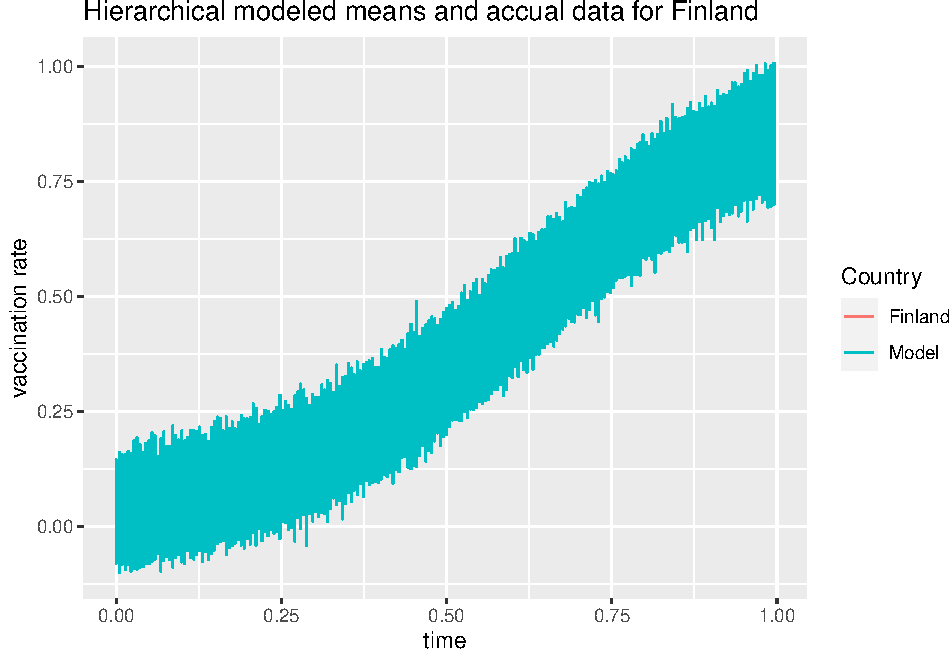
\includegraphics{bda_project_files/figure-latex/unnamed-chunk-30-1.pdf}

\begin{Shaded}
\begin{Highlighting}[]
\FunctionTok{qplot}\NormalTok{(fit\_sm}\SpecialCharTok{$}\NormalTok{ypred[,}\DecValTok{2}\NormalTok{], }\AttributeTok{geom=}\StringTok{"histogram"}\NormalTok{) }\SpecialCharTok{+}
    \FunctionTok{xlab}\NormalTok{(}\StringTok{""}\NormalTok{) }\SpecialCharTok{+}
    \FunctionTok{ylab}\NormalTok{(}\StringTok{""}\NormalTok{) }\SpecialCharTok{+}
    \FunctionTok{ggtitle}\NormalTok{(}\StringTok{"Prediction of vaccination rate in close future, Germany"}\NormalTok{)}
\end{Highlighting}
\end{Shaded}

\begin{verbatim}
## `stat_bin()` using `bins = 30`. Pick better value with `binwidth`.
\end{verbatim}

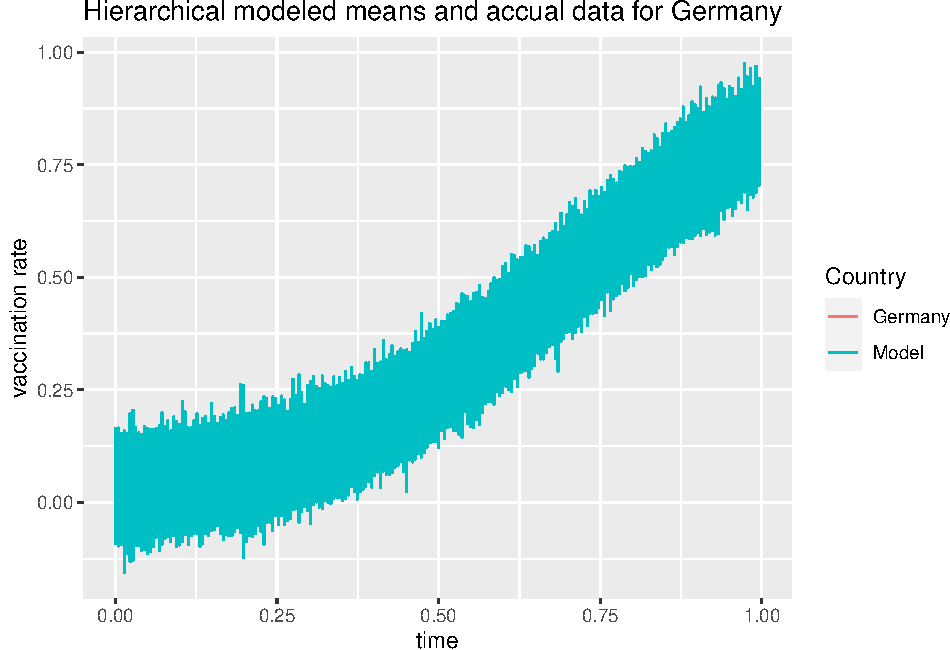
\includegraphics{bda_project_files/figure-latex/unnamed-chunk-31-1.pdf}

\begin{Shaded}
\begin{Highlighting}[]
\FunctionTok{qplot}\NormalTok{(fit\_sm}\SpecialCharTok{$}\NormalTok{ypred[,}\DecValTok{3}\NormalTok{], }\AttributeTok{geom=}\StringTok{"histogram"}\NormalTok{) }\SpecialCharTok{+}
    \FunctionTok{xlab}\NormalTok{(}\StringTok{""}\NormalTok{) }\SpecialCharTok{+}
    \FunctionTok{ylab}\NormalTok{(}\StringTok{""}\NormalTok{) }\SpecialCharTok{+}
    \FunctionTok{ggtitle}\NormalTok{(}\StringTok{"Prediction of vaccination rate in close future, Portugal"}\NormalTok{)}
\end{Highlighting}
\end{Shaded}

\begin{verbatim}
## `stat_bin()` using `bins = 30`. Pick better value with `binwidth`.
\end{verbatim}

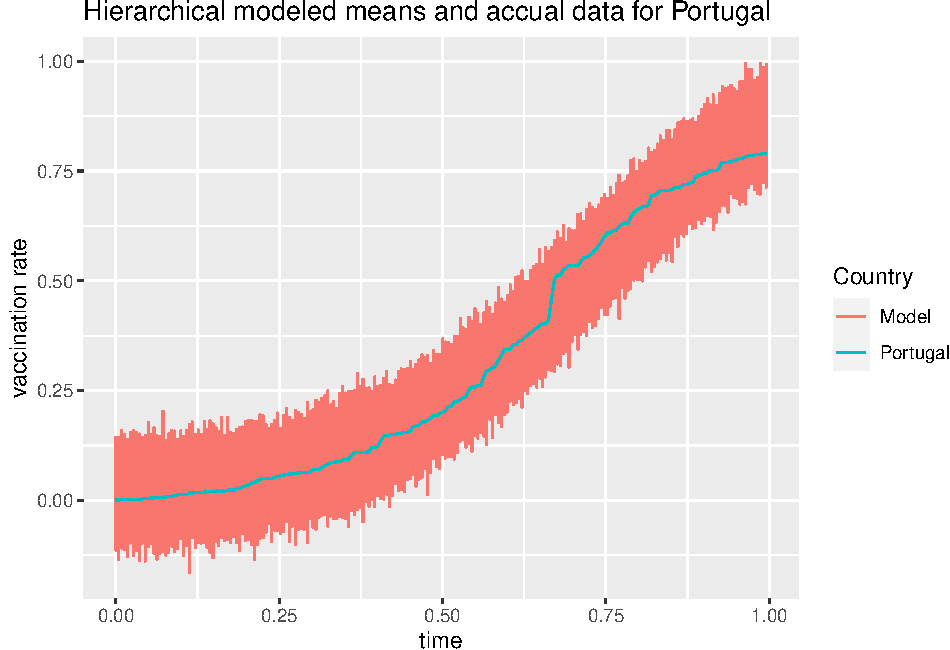
\includegraphics{bda_project_files/figure-latex/unnamed-chunk-32-1.pdf}

\begin{Shaded}
\begin{Highlighting}[]
\FunctionTok{qplot}\NormalTok{(fit\_sm}\SpecialCharTok{$}\NormalTok{ypred[,}\DecValTok{4}\NormalTok{], }\AttributeTok{geom=}\StringTok{"histogram"}\NormalTok{) }\SpecialCharTok{+}
    \FunctionTok{xlab}\NormalTok{(}\StringTok{""}\NormalTok{) }\SpecialCharTok{+}
    \FunctionTok{ylab}\NormalTok{(}\StringTok{""}\NormalTok{) }\SpecialCharTok{+}
    \FunctionTok{ggtitle}\NormalTok{(}\StringTok{"Prediction of vaccination rate in close future, Hongkong"}\NormalTok{)}
\end{Highlighting}
\end{Shaded}

\begin{verbatim}
## `stat_bin()` using `bins = 30`. Pick better value with `binwidth`.
\end{verbatim}

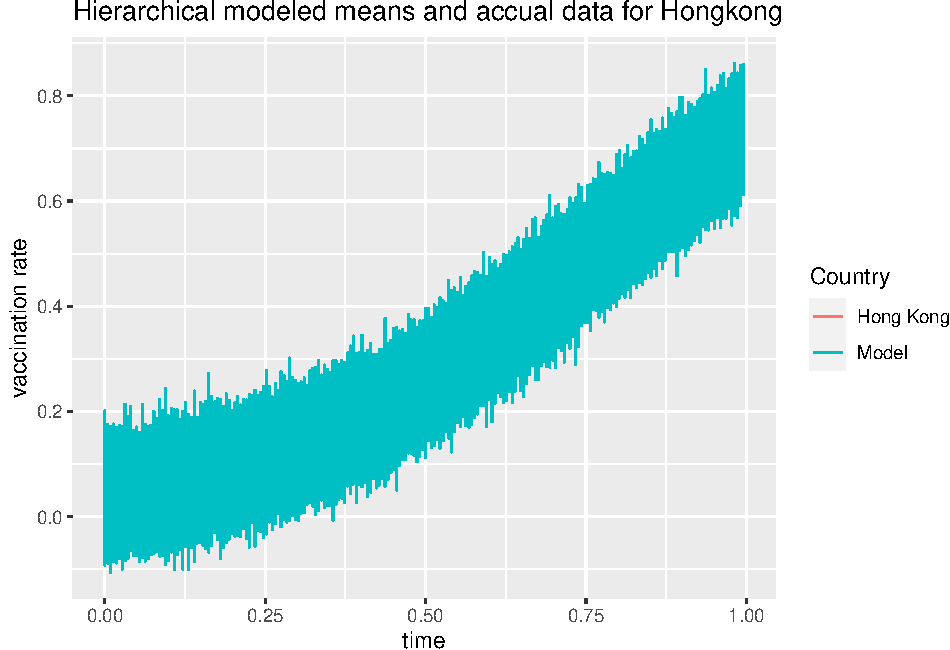
\includegraphics{bda_project_files/figure-latex/unnamed-chunk-33-1.pdf}

\begin{Shaded}
\begin{Highlighting}[]
\FunctionTok{qplot}\NormalTok{(fit\_sm}\SpecialCharTok{$}\NormalTok{ypred[,}\DecValTok{5}\NormalTok{], }\AttributeTok{geom=}\StringTok{"histogram"}\NormalTok{) }\SpecialCharTok{+}
    \FunctionTok{xlab}\NormalTok{(}\StringTok{""}\NormalTok{) }\SpecialCharTok{+}
    \FunctionTok{ylab}\NormalTok{(}\StringTok{""}\NormalTok{) }\SpecialCharTok{+}
    \FunctionTok{ggtitle}\NormalTok{(}\StringTok{"Prediction of vaccination rate in close future, Japan"}\NormalTok{)}
\end{Highlighting}
\end{Shaded}

\begin{verbatim}
## `stat_bin()` using `bins = 30`. Pick better value with `binwidth`.
\end{verbatim}

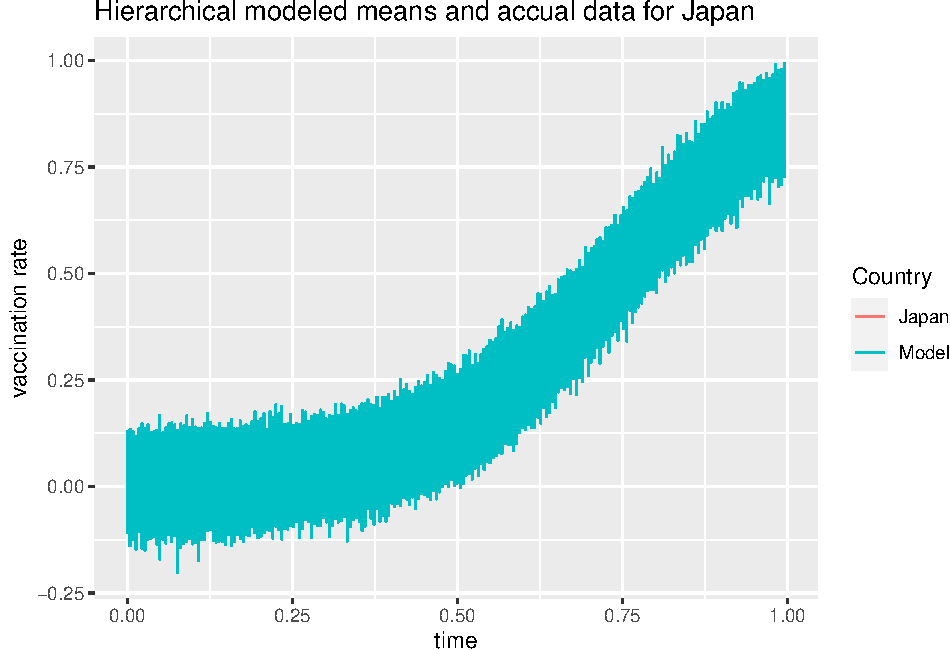
\includegraphics{bda_project_files/figure-latex/unnamed-chunk-34-1.pdf}

\begin{Shaded}
\begin{Highlighting}[]
\FunctionTok{cat}\NormalTok{(}\StringTok{"Mean of 4000 predictions for Finland: "}\NormalTok{, }\FunctionTok{mean}\NormalTok{(fit\_sm}\SpecialCharTok{$}\NormalTok{ypred[,}\DecValTok{1}\NormalTok{]),}\StringTok{\textquotesingle{}}\SpecialCharTok{\textbackslash{}n}\StringTok{\textquotesingle{}}\NormalTok{)}
\end{Highlighting}
\end{Shaded}

\begin{verbatim}
## Mean of 4000 predictions for Finland:  0.9141125
\end{verbatim}

\begin{Shaded}
\begin{Highlighting}[]
\FunctionTok{cat}\NormalTok{(}\StringTok{"Mean of 4000 predictions for Germany: "}\NormalTok{, }\FunctionTok{mean}\NormalTok{(fit\_sm}\SpecialCharTok{$}\NormalTok{ypred[,}\DecValTok{2}\NormalTok{]),}\StringTok{\textquotesingle{}}\SpecialCharTok{\textbackslash{}n}\StringTok{\textquotesingle{}}\NormalTok{)}
\end{Highlighting}
\end{Shaded}

\begin{verbatim}
## Mean of 4000 predictions for Germany:  0.8858833
\end{verbatim}

\begin{Shaded}
\begin{Highlighting}[]
\FunctionTok{cat}\NormalTok{(}\StringTok{"Mean of 4000 predictions for Portugal: "}\NormalTok{, }\FunctionTok{mean}\NormalTok{(fit\_sm}\SpecialCharTok{$}\NormalTok{ypred[,}\DecValTok{3}\NormalTok{]),}\StringTok{\textquotesingle{}}\SpecialCharTok{\textbackslash{}n}\StringTok{\textquotesingle{}}\NormalTok{)}
\end{Highlighting}
\end{Shaded}

\begin{verbatim}
## Mean of 4000 predictions for Portugal:  0.9191411
\end{verbatim}

\begin{Shaded}
\begin{Highlighting}[]
\FunctionTok{cat}\NormalTok{(}\StringTok{"Mean of 4000 predictions for Hong Kong: "}\NormalTok{, }\FunctionTok{mean}\NormalTok{(fit\_sm}\SpecialCharTok{$}\NormalTok{ypred[,}\DecValTok{4}\NormalTok{]),}\StringTok{\textquotesingle{}}\SpecialCharTok{\textbackslash{}n}\StringTok{\textquotesingle{}}\NormalTok{)}
\end{Highlighting}
\end{Shaded}

\begin{verbatim}
## Mean of 4000 predictions for Hong Kong:  0.8022076
\end{verbatim}

\begin{Shaded}
\begin{Highlighting}[]
\FunctionTok{cat}\NormalTok{(}\StringTok{"Mean of 4000 predictions for Japan: "}\NormalTok{, }\FunctionTok{mean}\NormalTok{(fit\_sm}\SpecialCharTok{$}\NormalTok{ypred[,}\DecValTok{5}\NormalTok{]),}\StringTok{\textquotesingle{}}\SpecialCharTok{\textbackslash{}n}\StringTok{\textquotesingle{}}\NormalTok{)}
\end{Highlighting}
\end{Shaded}

\begin{verbatim}
## Mean of 4000 predictions for Japan:  0.9302296
\end{verbatim}

\hypertarget{hierarchical-model}{%
\subsection{Hierarchical model}\label{hierarchical-model}}

Now we can evaluate the numbers for the hirachical model:

\begin{Shaded}
\begin{Highlighting}[]
\FunctionTok{qplot}\NormalTok{(fit\_hm}\SpecialCharTok{$}\NormalTok{ypred[,}\DecValTok{1}\NormalTok{], }\AttributeTok{geom=}\StringTok{"histogram"}\NormalTok{) }\SpecialCharTok{+}
    \FunctionTok{xlab}\NormalTok{(}\StringTok{""}\NormalTok{) }\SpecialCharTok{+}
    \FunctionTok{ylab}\NormalTok{(}\StringTok{""}\NormalTok{) }\SpecialCharTok{+}
    \FunctionTok{ggtitle}\NormalTok{(}\StringTok{"Prediction of vaccination rate in close future,Finland"}\NormalTok{)}
\end{Highlighting}
\end{Shaded}

\begin{verbatim}
## `stat_bin()` using `bins = 30`. Pick better value with `binwidth`.
\end{verbatim}

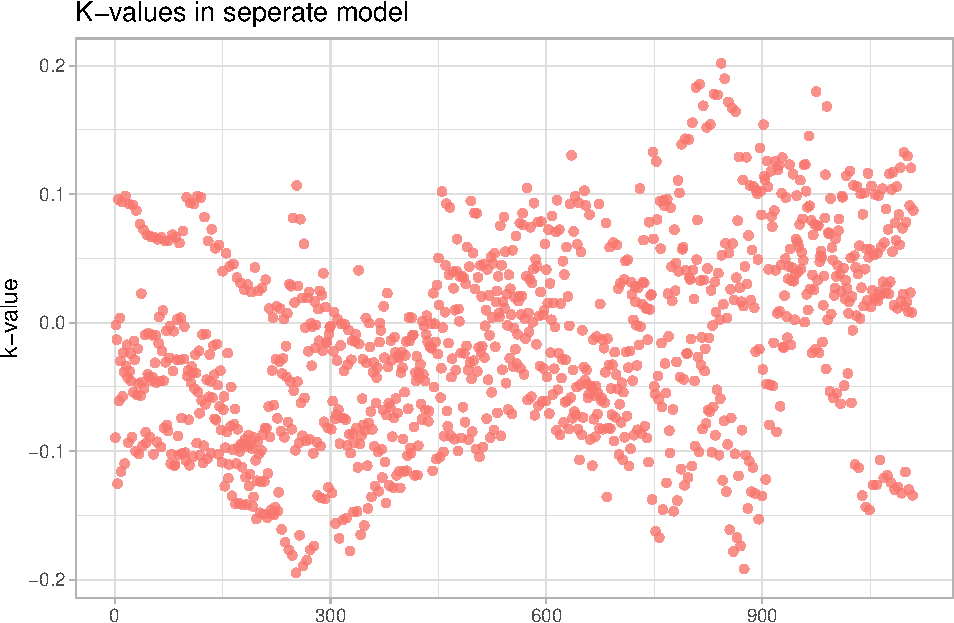
\includegraphics{bda_project_files/figure-latex/unnamed-chunk-36-1.pdf}

\begin{Shaded}
\begin{Highlighting}[]
\FunctionTok{qplot}\NormalTok{(fit\_hm}\SpecialCharTok{$}\NormalTok{ypred[,}\DecValTok{2}\NormalTok{], }\AttributeTok{geom=}\StringTok{"histogram"}\NormalTok{) }\SpecialCharTok{+}
    \FunctionTok{xlab}\NormalTok{(}\StringTok{""}\NormalTok{) }\SpecialCharTok{+}
    \FunctionTok{ylab}\NormalTok{(}\StringTok{""}\NormalTok{) }\SpecialCharTok{+}
    \FunctionTok{ggtitle}\NormalTok{(}\StringTok{"Prediction of vaccination rate in close future, Germany"}\NormalTok{)}
\end{Highlighting}
\end{Shaded}

\begin{verbatim}
## `stat_bin()` using `bins = 30`. Pick better value with `binwidth`.
\end{verbatim}

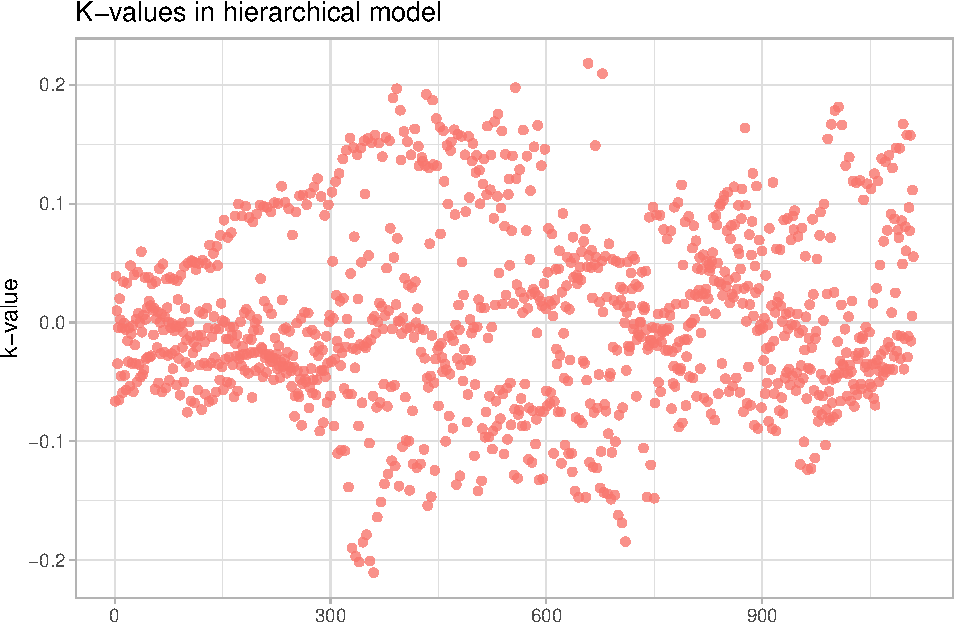
\includegraphics{bda_project_files/figure-latex/unnamed-chunk-37-1.pdf}

\begin{Shaded}
\begin{Highlighting}[]
\FunctionTok{qplot}\NormalTok{(fit\_hm}\SpecialCharTok{$}\NormalTok{ypred[,}\DecValTok{3}\NormalTok{], }\AttributeTok{geom=}\StringTok{"histogram"}\NormalTok{) }\SpecialCharTok{+}
    \FunctionTok{xlab}\NormalTok{(}\StringTok{""}\NormalTok{) }\SpecialCharTok{+}
    \FunctionTok{ylab}\NormalTok{(}\StringTok{""}\NormalTok{) }\SpecialCharTok{+}
    \FunctionTok{ggtitle}\NormalTok{(}\StringTok{"Prediction of vaccination rate in close future, Portugal"}\NormalTok{)}
\end{Highlighting}
\end{Shaded}

\begin{verbatim}
## `stat_bin()` using `bins = 30`. Pick better value with `binwidth`.
\end{verbatim}

\includegraphics{bda_project_files/figure-latex/unnamed-chunk-38-1.pdf}

\begin{Shaded}
\begin{Highlighting}[]
\FunctionTok{qplot}\NormalTok{(fit\_hm}\SpecialCharTok{$}\NormalTok{ypred[,}\DecValTok{4}\NormalTok{], }\AttributeTok{geom=}\StringTok{"histogram"}\NormalTok{) }\SpecialCharTok{+}
    \FunctionTok{xlab}\NormalTok{(}\StringTok{""}\NormalTok{) }\SpecialCharTok{+}
    \FunctionTok{ylab}\NormalTok{(}\StringTok{""}\NormalTok{) }\SpecialCharTok{+}
    \FunctionTok{ggtitle}\NormalTok{(}\StringTok{"Prediction of vaccination rate in close future, Hongkong"}\NormalTok{)}
\end{Highlighting}
\end{Shaded}

\begin{verbatim}
## `stat_bin()` using `bins = 30`. Pick better value with `binwidth`.
\end{verbatim}

\includegraphics{bda_project_files/figure-latex/unnamed-chunk-39-1.pdf}

\begin{Shaded}
\begin{Highlighting}[]
\FunctionTok{qplot}\NormalTok{(fit\_hm}\SpecialCharTok{$}\NormalTok{ypred[,}\DecValTok{5}\NormalTok{], }\AttributeTok{geom=}\StringTok{"histogram"}\NormalTok{) }\SpecialCharTok{+}
    \FunctionTok{xlab}\NormalTok{(}\StringTok{""}\NormalTok{) }\SpecialCharTok{+}
    \FunctionTok{ylab}\NormalTok{(}\StringTok{""}\NormalTok{) }\SpecialCharTok{+}
    \FunctionTok{ggtitle}\NormalTok{(}\StringTok{"Prediction of vaccination rate in close future, Japan"}\NormalTok{)}
\end{Highlighting}
\end{Shaded}

\begin{verbatim}
## `stat_bin()` using `bins = 30`. Pick better value with `binwidth`.
\end{verbatim}

\includegraphics{bda_project_files/figure-latex/unnamed-chunk-40-1.pdf}

\begin{Shaded}
\begin{Highlighting}[]
\FunctionTok{cat}\NormalTok{(}\StringTok{"Mean of 4000 predictions for Finland: "}\NormalTok{, }\FunctionTok{mean}\NormalTok{(fit\_hm}\SpecialCharTok{$}\NormalTok{ypred[,}\DecValTok{1}\NormalTok{]),}\StringTok{\textquotesingle{}}\SpecialCharTok{\textbackslash{}n}\StringTok{\textquotesingle{}}\NormalTok{)}
\end{Highlighting}
\end{Shaded}

\begin{verbatim}
## Mean of 4000 predictions for Finland:  0.9155683
\end{verbatim}

\begin{Shaded}
\begin{Highlighting}[]
\FunctionTok{cat}\NormalTok{(}\StringTok{"Mean of 4000 predictions for Germany: "}\NormalTok{, }\FunctionTok{mean}\NormalTok{(fit\_hm}\SpecialCharTok{$}\NormalTok{ypred[,}\DecValTok{2}\NormalTok{]),}\StringTok{\textquotesingle{}}\SpecialCharTok{\textbackslash{}n}\StringTok{\textquotesingle{}}\NormalTok{)}
\end{Highlighting}
\end{Shaded}

\begin{verbatim}
## Mean of 4000 predictions for Germany:  0.8852123
\end{verbatim}

\begin{Shaded}
\begin{Highlighting}[]
\FunctionTok{cat}\NormalTok{(}\StringTok{"Mean of 4000 predictions for Portugal: "}\NormalTok{, }\FunctionTok{mean}\NormalTok{(fit\_hm}\SpecialCharTok{$}\NormalTok{ypred[,}\DecValTok{3}\NormalTok{]),}\StringTok{\textquotesingle{}}\SpecialCharTok{\textbackslash{}n}\StringTok{\textquotesingle{}}\NormalTok{)}
\end{Highlighting}
\end{Shaded}

\begin{verbatim}
## Mean of 4000 predictions for Portugal:  0.9190773
\end{verbatim}

\begin{Shaded}
\begin{Highlighting}[]
\FunctionTok{cat}\NormalTok{(}\StringTok{"Mean of 4000 predictions for Hong Kong: "}\NormalTok{, }\FunctionTok{mean}\NormalTok{(fit\_hm}\SpecialCharTok{$}\NormalTok{ypred[,}\DecValTok{4}\NormalTok{]),}\StringTok{\textquotesingle{}}\SpecialCharTok{\textbackslash{}n}\StringTok{\textquotesingle{}}\NormalTok{)}
\end{Highlighting}
\end{Shaded}

\begin{verbatim}
## Mean of 4000 predictions for Hong Kong:  0.8019079
\end{verbatim}

\begin{Shaded}
\begin{Highlighting}[]
\FunctionTok{cat}\NormalTok{(}\StringTok{"Mean of 4000 predictions for Japan: "}\NormalTok{, }\FunctionTok{mean}\NormalTok{(fit\_hm}\SpecialCharTok{$}\NormalTok{ypred[,}\DecValTok{5}\NormalTok{]),}\StringTok{\textquotesingle{}}\SpecialCharTok{\textbackslash{}n}\StringTok{\textquotesingle{}}\NormalTok{)}
\end{Highlighting}
\end{Shaded}

\begin{verbatim}
## Mean of 4000 predictions for Japan:  0.9294456
\end{verbatim}

We need to be very carefull about the prediction of the vaccination
numbers. While it is nice having those predicitions, they are just
usefull.

\hypertarget{sensitivity-analysis-with-respect-to-prior-choices-i.e.-checking-whether-the-result-changes-a-lot-if-prior-is-changed}{%
\section{11. Sensitivity analysis with respect to prior choices
(i.e.~checking whether the result changes a lot if prior is
changed)}\label{sensitivity-analysis-with-respect-to-prior-choices-i.e.-checking-whether-the-result-changes-a-lot-if-prior-is-changed}}

\hypertarget{sensitivity-analysis-for-separate-model}{%
\subsection{Sensitivity analysis for separate
model}\label{sensitivity-analysis-for-separate-model}}

Lets consider the similar mathematical modeling for the separated model
and change some parameter values for the prior.

\[
  \begin{aligned}
y_{i j} \mid \mu_i, \sigma &\sim \operatorname{Normal}\left(\mu_i, \sigma\right) \\
\mu_i &\sim \operatorname{logit}(\alpha_i, \beta_i)\\
\sigma &\sim \text{inv}\chi^2(param_1)\\
\\
\alpha_i &\sim \text{inv}\chi^2(param_2) \\
\beta_i &\sim N(param_3, param_4) \\
\end{aligned}
\] Here, \(param_1\), \(param_2\), \(param_3\) and \(param_4\) are the
prior parameters that we are going to vary in our analysis. For the
comparison, we have our original values for the parameters as follows:

\[
\begin{aligned}
\sigma &\sim \text{inv}\chi^2(1) \qquad param_1 = 1\\
\alpha_i &\sim \text{inv}\chi^2(1) \qquad param_2 = 1\\
\beta_i &\sim N(0.5,1) \qquad param_3 = 0.5 \quad param_4 = 1\\
\end{aligned}
\] We will now create a stan model which is parameterized with the above
parameters.

\begin{Shaded}
\begin{Highlighting}[]
\NormalTok{seperated\_model\_parameterized }\OtherTok{\textless{}{-}} \StringTok{"}
\StringTok{functions \{}
\StringTok{  real[] logit\_transform(real[] x, real k, real x0) \{}
\StringTok{    int N = size(x);}
\StringTok{    real xtemp[N];}
\StringTok{    for (i in 1:N)\{}
\StringTok{      xtemp[i] = 1 / (1 + exp({-}k * (x[i] {-} x0)));}
\StringTok{    \}}
\StringTok{     return xtemp;}
\StringTok{  \}}
\StringTok{\}}

\StringTok{data \{}
\StringTok{    int\textless{}lower=0\textgreater{} J;}
\StringTok{    int\textless{}lower=1\textgreater{} M;}
\StringTok{    int\textless{}lower=0\textgreater{} N; // number of data points}
\StringTok{    real x[M,N]; // observation year}
\StringTok{    real y[M,N]; // observation number of drowned}
\StringTok{    real xpred;  // prediction year}
\StringTok{    real param1;}
\StringTok{    real param2;}
\StringTok{    real param3;}
\StringTok{    real param4;}
\StringTok{\}}

\StringTok{parameters \{}
\StringTok{  real alpha[M];}
\StringTok{  real beta[M];}
\StringTok{  real\textless{}lower = 0\textgreater{} sigma;}
\StringTok{\}}

\StringTok{transformed parameters \{}
\StringTok{  real mu[M,N];}
\StringTok{  for (i in 1:M)\{}
\StringTok{    mu[i,] = logit\_transform(x[i,],alpha[i], beta[i]);}
\StringTok{  \}}
\StringTok{\}}

\StringTok{model \{}
\StringTok{  for (i in 1:M)\{}
\StringTok{    // as prior we will change it to the same values}
\StringTok{    alpha[i] \textasciitilde{} inv\_chi\_square(param2);}
\StringTok{    beta[i] \textasciitilde{} normal(param3,param4);}
\StringTok{  \}}

\StringTok{  sigma \textasciitilde{} inv\_chi\_square(param1);}

\StringTok{  //likelihood}
\StringTok{  for (i in 1:M)\{}
\StringTok{    y[i,] \textasciitilde{} normal(mu[i,], sigma);}
\StringTok{  \}}
\StringTok{\}}

\StringTok{generated quantities \{}
\StringTok{  real ypred[M];}
\StringTok{  real t[1];}
\StringTok{  real log\_lik[M,N];}
\StringTok{  t[1] = xpred;}
\StringTok{  for (i in 1:M)\{}
\StringTok{    ypred[i] = normal\_rng(logit\_transform(t,alpha[i], beta[i])[1], sigma);}
\StringTok{  \}}

\StringTok{  //log{-}likelihood}
\StringTok{  for (i in 1:M) \{}
\StringTok{    for (j in 1:N) \{}
\StringTok{    log\_lik[i,j] = normal\_lpdf(y[i,j] | mu[i,j], sigma);}
\StringTok{    \}}
\StringTok{  \}}

\StringTok{\}}

\StringTok{"}
\end{Highlighting}
\end{Shaded}

\hypertarget{lets-fix-rest-of-the-parameters-so-that-we-can-change-the-sigma-prior-and-change-only-param_1}{%
\subsubsection{\texorpdfstring{Let's fix rest of the parameters so that
we can change the \(\sigma\) prior and change only
\(param_1\)}{Let's fix rest of the parameters so that we can change the \textbackslash sigma prior and change only param\_1}}\label{lets-fix-rest-of-the-parameters-so-that-we-can-change-the-sigma-prior-and-change-only-param_1}}

\begin{itemize}
\tightlist
\item
  \(param_1 = 0.1\)
\item
  \(param_1 = 0.5\)
\item
  \(param_1 = 10\)
\item
  \(param_1 = 100\)
\end{itemize}

\begin{Shaded}
\begin{Highlighting}[]
\NormalTok{xData }\OtherTok{\textless{}{-}} \FunctionTok{rbind}\NormalTok{(finland}\SpecialCharTok{$}\NormalTok{X,germany}\SpecialCharTok{$}\NormalTok{X,portugal}\SpecialCharTok{$}\NormalTok{X,hongkong}\SpecialCharTok{$}\NormalTok{X,japan}\SpecialCharTok{$}\NormalTok{X) }\CommentTok{\#(5,222)}
\NormalTok{yData }\OtherTok{\textless{}{-}}\FunctionTok{rbind}\NormalTok{(finland}\SpecialCharTok{$}\NormalTok{Y,germany}\SpecialCharTok{$}\NormalTok{Y,portugal}\SpecialCharTok{$}\NormalTok{Y,hongkong}\SpecialCharTok{$}\NormalTok{Y,japan}\SpecialCharTok{$}\NormalTok{Y) }\CommentTok{\#(5,222)}

\NormalTok{sigma\_priors }\OtherTok{\textless{}{-}} \FunctionTok{c}\NormalTok{(}\DecValTok{1}\NormalTok{, }\FloatTok{0.01}\NormalTok{, }\FloatTok{0.1}\NormalTok{, }\DecValTok{10}\NormalTok{, }\DecValTok{20}\NormalTok{)}

\NormalTok{fit\_smps }\OtherTok{\textless{}{-}} \FunctionTok{c}\NormalTok{()}

\ControlFlowTok{for}\NormalTok{(p }\ControlFlowTok{in}\NormalTok{ sigma\_priors) \{}
\NormalTok{  smp }\OtherTok{\textless{}{-}}\NormalTok{ rstan}\SpecialCharTok{::}\FunctionTok{stan\_model}\NormalTok{(}\AttributeTok{model\_code =}\NormalTok{ seperated\_model\_parameterized)}
\NormalTok{  stan\_data\_parameterized }\OtherTok{\textless{}{-}} \FunctionTok{list}\NormalTok{(}
      \AttributeTok{J =} \DecValTok{1}\NormalTok{,}
      \AttributeTok{N =} \FunctionTok{dim}\NormalTok{(xData)[}\DecValTok{2}\NormalTok{],}
      \AttributeTok{M =} \FunctionTok{dim}\NormalTok{(xData)[}\DecValTok{1}\NormalTok{],}
      \AttributeTok{y =}\NormalTok{ yData,}
      \AttributeTok{x =}\NormalTok{ xData,}
      \AttributeTok{xpred =} \FloatTok{1.1}\NormalTok{,}
      \AttributeTok{param1 =}\NormalTok{ p,}
      \AttributeTok{param2 =} \DecValTok{1}\NormalTok{,}
      \AttributeTok{param3 =} \FloatTok{0.5}\NormalTok{,}
      \AttributeTok{param4 =} \DecValTok{1}
\NormalTok{  )}
\NormalTok{  model\_separated\_parameterized }\OtherTok{\textless{}{-}}\NormalTok{ rstan}\SpecialCharTok{::}\FunctionTok{sampling}\NormalTok{(smp, }\AttributeTok{data =}\NormalTok{ stan\_data\_parameterized, }\AttributeTok{warmup=}\DecValTok{3000}\NormalTok{, }\AttributeTok{iter=}\DecValTok{4000}\NormalTok{)}
\NormalTok{  fit\_smp }\OtherTok{\textless{}{-}} \FunctionTok{extract}\NormalTok{(model\_separated\_parameterized, }\AttributeTok{permuted =} \ConstantTok{TRUE}\NormalTok{, }\AttributeTok{inc\_warmup =} \ConstantTok{FALSE}\NormalTok{)}
\NormalTok{  fit\_smps }\OtherTok{\textless{}{-}} \FunctionTok{rbind}\NormalTok{(fit\_smps, fit\_smp)}
\NormalTok{\}}
\end{Highlighting}
\end{Shaded}

\begin{verbatim}
## Trying to compile a simple C file
\end{verbatim}

\begin{verbatim}
## Warning in .local(object, ...): some chains had errors; consider specifying
## chains = 1 to debug
\end{verbatim}

\begin{verbatim}
## here are whatever error messages were returned
\end{verbatim}

Lets plot the different sigma values using a histogram.

\begin{Shaded}
\begin{Highlighting}[]
\NormalTok{values }\OtherTok{\textless{}{-}} \FunctionTok{c}\NormalTok{(fit\_smps[}\DecValTok{1}\NormalTok{,]}\SpecialCharTok{$}\NormalTok{sigma,}
\NormalTok{            fit\_smps[}\DecValTok{2}\NormalTok{,]}\SpecialCharTok{$}\NormalTok{sigma,}
\NormalTok{            fit\_smps[}\DecValTok{3}\NormalTok{,]}\SpecialCharTok{$}\NormalTok{sigma,}
\NormalTok{            fit\_smps[}\DecValTok{4}\NormalTok{,]}\SpecialCharTok{$}\NormalTok{sigma,}
\NormalTok{            fit\_smps[}\DecValTok{5}\NormalTok{,]}\SpecialCharTok{$}\NormalTok{sigma)}
\NormalTok{group }\OtherTok{\textless{}{-}} \FunctionTok{c}\NormalTok{(}\FunctionTok{rep}\NormalTok{(}\FunctionTok{sprintf}\NormalTok{(}\StringTok{"\%f"}\NormalTok{, sigma\_priors[}\DecValTok{1}\NormalTok{]), }\FunctionTok{length}\NormalTok{(fit\_smps[}\DecValTok{1}\NormalTok{,]}\SpecialCharTok{$}\NormalTok{sigma)),}
           \FunctionTok{rep}\NormalTok{(}\FunctionTok{sprintf}\NormalTok{(}\StringTok{"\%f"}\NormalTok{, sigma\_priors[}\DecValTok{2}\NormalTok{]), }\FunctionTok{length}\NormalTok{(fit\_smps[}\DecValTok{2}\NormalTok{,]}\SpecialCharTok{$}\NormalTok{sigma)),}
           \FunctionTok{rep}\NormalTok{(}\FunctionTok{sprintf}\NormalTok{(}\StringTok{"\%f"}\NormalTok{, sigma\_priors[}\DecValTok{3}\NormalTok{]), }\FunctionTok{length}\NormalTok{(fit\_smps[}\DecValTok{3}\NormalTok{,]}\SpecialCharTok{$}\NormalTok{sigma)),}
           \FunctionTok{rep}\NormalTok{(}\FunctionTok{sprintf}\NormalTok{(}\StringTok{"\%f"}\NormalTok{, sigma\_priors[}\DecValTok{4}\NormalTok{]), }\FunctionTok{length}\NormalTok{(fit\_smps[}\DecValTok{4}\NormalTok{,]}\SpecialCharTok{$}\NormalTok{sigma)),}
           \FunctionTok{rep}\NormalTok{(}\FunctionTok{sprintf}\NormalTok{(}\StringTok{"\%f"}\NormalTok{, sigma\_priors[}\DecValTok{5}\NormalTok{]), }\FunctionTok{length}\NormalTok{(fit\_smps[}\DecValTok{5}\NormalTok{,]}\SpecialCharTok{$}\NormalTok{sigma)))}
\NormalTok{data }\OtherTok{\textless{}{-}} \FunctionTok{data.frame}\NormalTok{(}\AttributeTok{values =}\NormalTok{ values, }\AttributeTok{group =}\NormalTok{ group)}

\FunctionTok{ggplot}\NormalTok{(data, }\FunctionTok{aes}\NormalTok{(}\AttributeTok{x =}\NormalTok{ values, }\AttributeTok{fill =}\NormalTok{ group)) }\SpecialCharTok{+}                       \CommentTok{\# Draw overlaying histogram}
  \FunctionTok{geom\_histogram}\NormalTok{(}\AttributeTok{position =} \StringTok{"identity"}\NormalTok{, }\AttributeTok{alpha =} \FloatTok{0.2}\NormalTok{, }\AttributeTok{bins =} \DecValTok{50}\NormalTok{)}
\end{Highlighting}
\end{Shaded}

\includegraphics{bda_project_files/figure-latex/unnamed-chunk-44-1.pdf}

\hypertarget{lets-fix-rest-of-the-parameters-so-that-we-can-change-the-alpha-prior-and-change-only-param_2}{%
\subsubsection{\texorpdfstring{Let's fix rest of the parameters so that
we can change the \(\alpha\) prior and change only
\(param_2\)}{Let's fix rest of the parameters so that we can change the \textbackslash alpha prior and change only param\_2}}\label{lets-fix-rest-of-the-parameters-so-that-we-can-change-the-alpha-prior-and-change-only-param_2}}

\begin{itemize}
\tightlist
\item
  \(param_2 = 0.1\)
\item
  \(param_2 = 0.5\)
\item
  \(param_2 = 10\)
\item
  \(param_2 = 100\)
\end{itemize}

\begin{Shaded}
\begin{Highlighting}[]
\NormalTok{xData }\OtherTok{\textless{}{-}} \FunctionTok{rbind}\NormalTok{(finland}\SpecialCharTok{$}\NormalTok{X,germany}\SpecialCharTok{$}\NormalTok{X,portugal}\SpecialCharTok{$}\NormalTok{X,hongkong}\SpecialCharTok{$}\NormalTok{X,japan}\SpecialCharTok{$}\NormalTok{X) }\CommentTok{\#(5,222)}
\NormalTok{yData }\OtherTok{\textless{}{-}}\FunctionTok{rbind}\NormalTok{(finland}\SpecialCharTok{$}\NormalTok{Y,germany}\SpecialCharTok{$}\NormalTok{Y,portugal}\SpecialCharTok{$}\NormalTok{Y,hongkong}\SpecialCharTok{$}\NormalTok{Y,japan}\SpecialCharTok{$}\NormalTok{Y) }\CommentTok{\#(5,222)}

\NormalTok{alpha\_priors }\OtherTok{\textless{}{-}} \FunctionTok{c}\NormalTok{(}\DecValTok{1}\NormalTok{, }\FloatTok{0.01}\NormalTok{, }\FloatTok{0.1}\NormalTok{, }\DecValTok{10}\NormalTok{, }\DecValTok{20}\NormalTok{)}

\NormalTok{fit\_smps }\OtherTok{\textless{}{-}} \FunctionTok{c}\NormalTok{()}

\ControlFlowTok{for}\NormalTok{(p }\ControlFlowTok{in}\NormalTok{ sigma\_priors) \{}
\NormalTok{  smp }\OtherTok{\textless{}{-}}\NormalTok{ rstan}\SpecialCharTok{::}\FunctionTok{stan\_model}\NormalTok{(}\AttributeTok{model\_code =}\NormalTok{ seperated\_model\_parameterized)}
\NormalTok{  stan\_data\_parameterized }\OtherTok{\textless{}{-}} \FunctionTok{list}\NormalTok{(}
      \AttributeTok{J =} \DecValTok{1}\NormalTok{,}
      \AttributeTok{N =} \FunctionTok{dim}\NormalTok{(xData)[}\DecValTok{2}\NormalTok{],}
      \AttributeTok{M =} \FunctionTok{dim}\NormalTok{(xData)[}\DecValTok{1}\NormalTok{],}
      \AttributeTok{y =}\NormalTok{ yData,}
      \AttributeTok{x =}\NormalTok{ xData,}
      \AttributeTok{xpred =} \FloatTok{1.1}\NormalTok{,}
      \AttributeTok{param1 =} \DecValTok{1}\NormalTok{,}
      \AttributeTok{param2 =}\NormalTok{ p,}
      \AttributeTok{param3 =} \FloatTok{0.5}\NormalTok{,}
      \AttributeTok{param4 =} \DecValTok{1}
\NormalTok{  )}
\NormalTok{  model\_separated\_parameterized }\OtherTok{\textless{}{-}}\NormalTok{ rstan}\SpecialCharTok{::}\FunctionTok{sampling}\NormalTok{(smp, }\AttributeTok{data =}\NormalTok{ stan\_data\_parameterized, }\AttributeTok{warmup=}\DecValTok{3000}\NormalTok{, }\AttributeTok{iter=}\DecValTok{4000}\NormalTok{)}
\NormalTok{  fit\_smp }\OtherTok{\textless{}{-}} \FunctionTok{extract}\NormalTok{(model\_separated\_parameterized, }\AttributeTok{permuted =} \ConstantTok{TRUE}\NormalTok{, }\AttributeTok{inc\_warmup =} \ConstantTok{FALSE}\NormalTok{)}
\NormalTok{  fit\_smps }\OtherTok{\textless{}{-}} \FunctionTok{rbind}\NormalTok{(fit\_smps, fit\_smp)}
\NormalTok{\}}
\end{Highlighting}
\end{Shaded}

\begin{verbatim}
## Warning in .local(object, ...): some chains had errors; consider specifying
## chains = 1 to debug
\end{verbatim}

\begin{verbatim}
## here are whatever error messages were returned
\end{verbatim}

Lets plot the different alpha values using a histogram.

\begin{Shaded}
\begin{Highlighting}[]
\NormalTok{values }\OtherTok{\textless{}{-}} \FunctionTok{c}\NormalTok{(fit\_smps[}\DecValTok{1}\NormalTok{,]}\SpecialCharTok{$}\NormalTok{alpha[,}\DecValTok{1}\NormalTok{],}
\NormalTok{            fit\_smps[}\DecValTok{2}\NormalTok{,]}\SpecialCharTok{$}\NormalTok{alpha[,}\DecValTok{1}\NormalTok{],}
\NormalTok{            fit\_smps[}\DecValTok{3}\NormalTok{,]}\SpecialCharTok{$}\NormalTok{alpha[,}\DecValTok{1}\NormalTok{],}
\NormalTok{            fit\_smps[}\DecValTok{4}\NormalTok{,]}\SpecialCharTok{$}\NormalTok{alpha[,}\DecValTok{1}\NormalTok{],}
\NormalTok{            fit\_smps[}\DecValTok{5}\NormalTok{,]}\SpecialCharTok{$}\NormalTok{alpha[,}\DecValTok{1}\NormalTok{])}
\NormalTok{group }\OtherTok{\textless{}{-}} \FunctionTok{c}\NormalTok{(}\FunctionTok{rep}\NormalTok{(}\FunctionTok{sprintf}\NormalTok{(}\StringTok{"\%f"}\NormalTok{, alpha\_priors[}\DecValTok{1}\NormalTok{]), }\FunctionTok{length}\NormalTok{(fit\_smps[}\DecValTok{1}\NormalTok{,]}\SpecialCharTok{$}\NormalTok{alpha[,}\DecValTok{1}\NormalTok{])),}
           \FunctionTok{rep}\NormalTok{(}\FunctionTok{sprintf}\NormalTok{(}\StringTok{"\%f"}\NormalTok{, alpha\_priors[}\DecValTok{2}\NormalTok{]), }\FunctionTok{length}\NormalTok{(fit\_smps[}\DecValTok{2}\NormalTok{,]}\SpecialCharTok{$}\NormalTok{alpha[,}\DecValTok{1}\NormalTok{])),}
           \FunctionTok{rep}\NormalTok{(}\FunctionTok{sprintf}\NormalTok{(}\StringTok{"\%f"}\NormalTok{, alpha\_priors[}\DecValTok{3}\NormalTok{]), }\FunctionTok{length}\NormalTok{(fit\_smps[}\DecValTok{3}\NormalTok{,]}\SpecialCharTok{$}\NormalTok{alpha[,}\DecValTok{1}\NormalTok{])),}
           \FunctionTok{rep}\NormalTok{(}\FunctionTok{sprintf}\NormalTok{(}\StringTok{"\%f"}\NormalTok{, alpha\_priors[}\DecValTok{4}\NormalTok{]), }\FunctionTok{length}\NormalTok{(fit\_smps[}\DecValTok{4}\NormalTok{,]}\SpecialCharTok{$}\NormalTok{alpha[,}\DecValTok{1}\NormalTok{])),}
           \FunctionTok{rep}\NormalTok{(}\FunctionTok{sprintf}\NormalTok{(}\StringTok{"\%f"}\NormalTok{, alpha\_priors[}\DecValTok{5}\NormalTok{]), }\FunctionTok{length}\NormalTok{(fit\_smps[}\DecValTok{5}\NormalTok{,]}\SpecialCharTok{$}\NormalTok{alpha[,}\DecValTok{1}\NormalTok{])))}
\NormalTok{data }\OtherTok{\textless{}{-}} \FunctionTok{data.frame}\NormalTok{(}\AttributeTok{values =}\NormalTok{ values, }\AttributeTok{group =}\NormalTok{ group)}

\FunctionTok{ggplot}\NormalTok{(data, }\FunctionTok{aes}\NormalTok{(}\AttributeTok{x =}\NormalTok{ values, }\AttributeTok{fill =}\NormalTok{ group)) }\SpecialCharTok{+} \FunctionTok{ggtitle}\NormalTok{(}\StringTok{"Plot of different alpha priors for Finland"}\NormalTok{) }\SpecialCharTok{+}
  \FunctionTok{geom\_histogram}\NormalTok{(}\AttributeTok{position =} \StringTok{"identity"}\NormalTok{, }\AttributeTok{alpha =} \FloatTok{0.2}\NormalTok{, }\AttributeTok{bins =} \DecValTok{50}\NormalTok{)}
\end{Highlighting}
\end{Shaded}

\includegraphics{bda_project_files/figure-latex/unnamed-chunk-46-1.pdf}

\begin{Shaded}
\begin{Highlighting}[]
\NormalTok{values }\OtherTok{\textless{}{-}} \FunctionTok{c}\NormalTok{(fit\_smps[}\DecValTok{1}\NormalTok{,]}\SpecialCharTok{$}\NormalTok{alpha[,}\DecValTok{2}\NormalTok{],}
\NormalTok{            fit\_smps[}\DecValTok{2}\NormalTok{,]}\SpecialCharTok{$}\NormalTok{alpha[,}\DecValTok{2}\NormalTok{],}
\NormalTok{            fit\_smps[}\DecValTok{3}\NormalTok{,]}\SpecialCharTok{$}\NormalTok{alpha[,}\DecValTok{2}\NormalTok{],}
\NormalTok{            fit\_smps[}\DecValTok{4}\NormalTok{,]}\SpecialCharTok{$}\NormalTok{alpha[,}\DecValTok{2}\NormalTok{],}
\NormalTok{            fit\_smps[}\DecValTok{5}\NormalTok{,]}\SpecialCharTok{$}\NormalTok{alpha[,}\DecValTok{2}\NormalTok{])}
\NormalTok{group }\OtherTok{\textless{}{-}} \FunctionTok{c}\NormalTok{(}\FunctionTok{rep}\NormalTok{(}\FunctionTok{sprintf}\NormalTok{(}\StringTok{"\%f"}\NormalTok{, alpha\_priors[}\DecValTok{1}\NormalTok{]), }\FunctionTok{length}\NormalTok{(fit\_smps[}\DecValTok{1}\NormalTok{,]}\SpecialCharTok{$}\NormalTok{alpha[,}\DecValTok{2}\NormalTok{])),}
           \FunctionTok{rep}\NormalTok{(}\FunctionTok{sprintf}\NormalTok{(}\StringTok{"\%f"}\NormalTok{, alpha\_priors[}\DecValTok{2}\NormalTok{]), }\FunctionTok{length}\NormalTok{(fit\_smps[}\DecValTok{2}\NormalTok{,]}\SpecialCharTok{$}\NormalTok{alpha[,}\DecValTok{2}\NormalTok{])),}
           \FunctionTok{rep}\NormalTok{(}\FunctionTok{sprintf}\NormalTok{(}\StringTok{"\%f"}\NormalTok{, alpha\_priors[}\DecValTok{3}\NormalTok{]), }\FunctionTok{length}\NormalTok{(fit\_smps[}\DecValTok{3}\NormalTok{,]}\SpecialCharTok{$}\NormalTok{alpha[,}\DecValTok{2}\NormalTok{])),}
           \FunctionTok{rep}\NormalTok{(}\FunctionTok{sprintf}\NormalTok{(}\StringTok{"\%f"}\NormalTok{, alpha\_priors[}\DecValTok{4}\NormalTok{]), }\FunctionTok{length}\NormalTok{(fit\_smps[}\DecValTok{4}\NormalTok{,]}\SpecialCharTok{$}\NormalTok{alpha[,}\DecValTok{2}\NormalTok{])),}
           \FunctionTok{rep}\NormalTok{(}\FunctionTok{sprintf}\NormalTok{(}\StringTok{"\%f"}\NormalTok{, alpha\_priors[}\DecValTok{5}\NormalTok{]), }\FunctionTok{length}\NormalTok{(fit\_smps[}\DecValTok{5}\NormalTok{,]}\SpecialCharTok{$}\NormalTok{alpha[,}\DecValTok{2}\NormalTok{])))}
\NormalTok{data }\OtherTok{\textless{}{-}} \FunctionTok{data.frame}\NormalTok{(}\AttributeTok{values =}\NormalTok{ values, }\AttributeTok{group =}\NormalTok{ group)}

\FunctionTok{ggplot}\NormalTok{(data, }\FunctionTok{aes}\NormalTok{(}\AttributeTok{x =}\NormalTok{ values, }\AttributeTok{fill =}\NormalTok{ group)) }\SpecialCharTok{+} \FunctionTok{ggtitle}\NormalTok{(}\StringTok{"Plot of different alpha priors for Germany"}\NormalTok{) }\SpecialCharTok{+}
  \FunctionTok{geom\_histogram}\NormalTok{(}\AttributeTok{position =} \StringTok{"identity"}\NormalTok{, }\AttributeTok{alpha =} \FloatTok{0.2}\NormalTok{, }\AttributeTok{bins =} \DecValTok{50}\NormalTok{)}
\end{Highlighting}
\end{Shaded}

\includegraphics{bda_project_files/figure-latex/unnamed-chunk-47-1.pdf}

\begin{Shaded}
\begin{Highlighting}[]
\NormalTok{values }\OtherTok{\textless{}{-}} \FunctionTok{c}\NormalTok{(fit\_smps[}\DecValTok{1}\NormalTok{,]}\SpecialCharTok{$}\NormalTok{alpha[,}\DecValTok{3}\NormalTok{],}
\NormalTok{            fit\_smps[}\DecValTok{2}\NormalTok{,]}\SpecialCharTok{$}\NormalTok{alpha[,}\DecValTok{3}\NormalTok{],}
\NormalTok{            fit\_smps[}\DecValTok{3}\NormalTok{,]}\SpecialCharTok{$}\NormalTok{alpha[,}\DecValTok{3}\NormalTok{],}
\NormalTok{            fit\_smps[}\DecValTok{4}\NormalTok{,]}\SpecialCharTok{$}\NormalTok{alpha[,}\DecValTok{3}\NormalTok{],}
\NormalTok{            fit\_smps[}\DecValTok{5}\NormalTok{,]}\SpecialCharTok{$}\NormalTok{alpha[,}\DecValTok{3}\NormalTok{])}
\NormalTok{group }\OtherTok{\textless{}{-}} \FunctionTok{c}\NormalTok{(}\FunctionTok{rep}\NormalTok{(}\FunctionTok{sprintf}\NormalTok{(}\StringTok{"\%f"}\NormalTok{, alpha\_priors[}\DecValTok{1}\NormalTok{]), }\FunctionTok{length}\NormalTok{(fit\_smps[}\DecValTok{1}\NormalTok{,]}\SpecialCharTok{$}\NormalTok{alpha[,}\DecValTok{3}\NormalTok{])),}
           \FunctionTok{rep}\NormalTok{(}\FunctionTok{sprintf}\NormalTok{(}\StringTok{"\%f"}\NormalTok{, alpha\_priors[}\DecValTok{2}\NormalTok{]), }\FunctionTok{length}\NormalTok{(fit\_smps[}\DecValTok{2}\NormalTok{,]}\SpecialCharTok{$}\NormalTok{alpha[,}\DecValTok{3}\NormalTok{])),}
           \FunctionTok{rep}\NormalTok{(}\FunctionTok{sprintf}\NormalTok{(}\StringTok{"\%f"}\NormalTok{, alpha\_priors[}\DecValTok{3}\NormalTok{]), }\FunctionTok{length}\NormalTok{(fit\_smps[}\DecValTok{3}\NormalTok{,]}\SpecialCharTok{$}\NormalTok{alpha[,}\DecValTok{3}\NormalTok{])),}
           \FunctionTok{rep}\NormalTok{(}\FunctionTok{sprintf}\NormalTok{(}\StringTok{"\%f"}\NormalTok{, alpha\_priors[}\DecValTok{4}\NormalTok{]), }\FunctionTok{length}\NormalTok{(fit\_smps[}\DecValTok{4}\NormalTok{,]}\SpecialCharTok{$}\NormalTok{alpha[,}\DecValTok{3}\NormalTok{])),}
           \FunctionTok{rep}\NormalTok{(}\FunctionTok{sprintf}\NormalTok{(}\StringTok{"\%f"}\NormalTok{, alpha\_priors[}\DecValTok{5}\NormalTok{]), }\FunctionTok{length}\NormalTok{(fit\_smps[}\DecValTok{5}\NormalTok{,]}\SpecialCharTok{$}\NormalTok{alpha[,}\DecValTok{3}\NormalTok{])))}
\NormalTok{data }\OtherTok{\textless{}{-}} \FunctionTok{data.frame}\NormalTok{(}\AttributeTok{values =}\NormalTok{ values, }\AttributeTok{group =}\NormalTok{ group)}

\FunctionTok{ggplot}\NormalTok{(data, }\FunctionTok{aes}\NormalTok{(}\AttributeTok{x =}\NormalTok{ values, }\AttributeTok{fill =}\NormalTok{ group)) }\SpecialCharTok{+} \FunctionTok{ggtitle}\NormalTok{(}\StringTok{"Plot of different alpha priors for Portugal"}\NormalTok{) }\SpecialCharTok{+}
  \FunctionTok{geom\_histogram}\NormalTok{(}\AttributeTok{position =} \StringTok{"identity"}\NormalTok{, }\AttributeTok{alpha =} \FloatTok{0.2}\NormalTok{, }\AttributeTok{bins =} \DecValTok{50}\NormalTok{)}
\end{Highlighting}
\end{Shaded}

\includegraphics{bda_project_files/figure-latex/unnamed-chunk-48-1.pdf}

\begin{Shaded}
\begin{Highlighting}[]
\NormalTok{values }\OtherTok{\textless{}{-}} \FunctionTok{c}\NormalTok{(fit\_smps[}\DecValTok{1}\NormalTok{,]}\SpecialCharTok{$}\NormalTok{alpha[,}\DecValTok{4}\NormalTok{],}
\NormalTok{            fit\_smps[}\DecValTok{2}\NormalTok{,]}\SpecialCharTok{$}\NormalTok{alpha[,}\DecValTok{4}\NormalTok{],}
\NormalTok{            fit\_smps[}\DecValTok{3}\NormalTok{,]}\SpecialCharTok{$}\NormalTok{alpha[,}\DecValTok{4}\NormalTok{],}
\NormalTok{            fit\_smps[}\DecValTok{4}\NormalTok{,]}\SpecialCharTok{$}\NormalTok{alpha[,}\DecValTok{4}\NormalTok{],}
\NormalTok{            fit\_smps[}\DecValTok{5}\NormalTok{,]}\SpecialCharTok{$}\NormalTok{alpha[,}\DecValTok{4}\NormalTok{])}
\NormalTok{group }\OtherTok{\textless{}{-}} \FunctionTok{c}\NormalTok{(}\FunctionTok{rep}\NormalTok{(}\FunctionTok{sprintf}\NormalTok{(}\StringTok{"\%f"}\NormalTok{, alpha\_priors[}\DecValTok{1}\NormalTok{]), }\FunctionTok{length}\NormalTok{(fit\_smps[}\DecValTok{1}\NormalTok{,]}\SpecialCharTok{$}\NormalTok{alpha[,}\DecValTok{4}\NormalTok{])),}
           \FunctionTok{rep}\NormalTok{(}\FunctionTok{sprintf}\NormalTok{(}\StringTok{"\%f"}\NormalTok{, alpha\_priors[}\DecValTok{2}\NormalTok{]), }\FunctionTok{length}\NormalTok{(fit\_smps[}\DecValTok{2}\NormalTok{,]}\SpecialCharTok{$}\NormalTok{alpha[,}\DecValTok{4}\NormalTok{])),}
           \FunctionTok{rep}\NormalTok{(}\FunctionTok{sprintf}\NormalTok{(}\StringTok{"\%f"}\NormalTok{, alpha\_priors[}\DecValTok{3}\NormalTok{]), }\FunctionTok{length}\NormalTok{(fit\_smps[}\DecValTok{3}\NormalTok{,]}\SpecialCharTok{$}\NormalTok{alpha[,}\DecValTok{4}\NormalTok{])),}
           \FunctionTok{rep}\NormalTok{(}\FunctionTok{sprintf}\NormalTok{(}\StringTok{"\%f"}\NormalTok{, alpha\_priors[}\DecValTok{4}\NormalTok{]), }\FunctionTok{length}\NormalTok{(fit\_smps[}\DecValTok{4}\NormalTok{,]}\SpecialCharTok{$}\NormalTok{alpha[,}\DecValTok{4}\NormalTok{])),}
           \FunctionTok{rep}\NormalTok{(}\FunctionTok{sprintf}\NormalTok{(}\StringTok{"\%f"}\NormalTok{, alpha\_priors[}\DecValTok{5}\NormalTok{]), }\FunctionTok{length}\NormalTok{(fit\_smps[}\DecValTok{5}\NormalTok{,]}\SpecialCharTok{$}\NormalTok{alpha[,}\DecValTok{4}\NormalTok{])))}
\NormalTok{data }\OtherTok{\textless{}{-}} \FunctionTok{data.frame}\NormalTok{(}\AttributeTok{values =}\NormalTok{ values, }\AttributeTok{group =}\NormalTok{ group)}

\FunctionTok{ggplot}\NormalTok{(data, }\FunctionTok{aes}\NormalTok{(}\AttributeTok{x =}\NormalTok{ values, }\AttributeTok{fill =}\NormalTok{ group)) }\SpecialCharTok{+} \FunctionTok{ggtitle}\NormalTok{(}\StringTok{"Plot of different alpha priors for Hong Kong"}\NormalTok{) }\SpecialCharTok{+}
  \FunctionTok{geom\_histogram}\NormalTok{(}\AttributeTok{position =} \StringTok{"identity"}\NormalTok{, }\AttributeTok{alpha =} \FloatTok{0.2}\NormalTok{, }\AttributeTok{bins =} \DecValTok{50}\NormalTok{)}
\end{Highlighting}
\end{Shaded}

\includegraphics{bda_project_files/figure-latex/unnamed-chunk-49-1.pdf}

\begin{Shaded}
\begin{Highlighting}[]
\NormalTok{values }\OtherTok{\textless{}{-}} \FunctionTok{c}\NormalTok{(fit\_smps[}\DecValTok{1}\NormalTok{,]}\SpecialCharTok{$}\NormalTok{alpha[,}\DecValTok{5}\NormalTok{],}
\NormalTok{            fit\_smps[}\DecValTok{2}\NormalTok{,]}\SpecialCharTok{$}\NormalTok{alpha[,}\DecValTok{5}\NormalTok{],}
\NormalTok{            fit\_smps[}\DecValTok{3}\NormalTok{,]}\SpecialCharTok{$}\NormalTok{alpha[,}\DecValTok{5}\NormalTok{],}
\NormalTok{            fit\_smps[}\DecValTok{4}\NormalTok{,]}\SpecialCharTok{$}\NormalTok{alpha[,}\DecValTok{5}\NormalTok{],}
\NormalTok{            fit\_smps[}\DecValTok{5}\NormalTok{,]}\SpecialCharTok{$}\NormalTok{alpha[,}\DecValTok{5}\NormalTok{])}
\NormalTok{group }\OtherTok{\textless{}{-}} \FunctionTok{c}\NormalTok{(}\FunctionTok{rep}\NormalTok{(}\FunctionTok{sprintf}\NormalTok{(}\StringTok{"\%f"}\NormalTok{, alpha\_priors[}\DecValTok{1}\NormalTok{]), }\FunctionTok{length}\NormalTok{(fit\_smps[}\DecValTok{1}\NormalTok{,]}\SpecialCharTok{$}\NormalTok{alpha[,}\DecValTok{5}\NormalTok{])),}
           \FunctionTok{rep}\NormalTok{(}\FunctionTok{sprintf}\NormalTok{(}\StringTok{"\%f"}\NormalTok{, alpha\_priors[}\DecValTok{2}\NormalTok{]), }\FunctionTok{length}\NormalTok{(fit\_smps[}\DecValTok{2}\NormalTok{,]}\SpecialCharTok{$}\NormalTok{alpha[,}\DecValTok{5}\NormalTok{])),}
           \FunctionTok{rep}\NormalTok{(}\FunctionTok{sprintf}\NormalTok{(}\StringTok{"\%f"}\NormalTok{, alpha\_priors[}\DecValTok{3}\NormalTok{]), }\FunctionTok{length}\NormalTok{(fit\_smps[}\DecValTok{3}\NormalTok{,]}\SpecialCharTok{$}\NormalTok{alpha[,}\DecValTok{5}\NormalTok{])),}
           \FunctionTok{rep}\NormalTok{(}\FunctionTok{sprintf}\NormalTok{(}\StringTok{"\%f"}\NormalTok{, alpha\_priors[}\DecValTok{4}\NormalTok{]), }\FunctionTok{length}\NormalTok{(fit\_smps[}\DecValTok{4}\NormalTok{,]}\SpecialCharTok{$}\NormalTok{alpha[,}\DecValTok{5}\NormalTok{])),}
           \FunctionTok{rep}\NormalTok{(}\FunctionTok{sprintf}\NormalTok{(}\StringTok{"\%f"}\NormalTok{, alpha\_priors[}\DecValTok{5}\NormalTok{]), }\FunctionTok{length}\NormalTok{(fit\_smps[}\DecValTok{5}\NormalTok{,]}\SpecialCharTok{$}\NormalTok{alpha[,}\DecValTok{5}\NormalTok{])))}
\NormalTok{data }\OtherTok{\textless{}{-}} \FunctionTok{data.frame}\NormalTok{(}\AttributeTok{values =}\NormalTok{ values, }\AttributeTok{group =}\NormalTok{ group)}

\FunctionTok{ggplot}\NormalTok{(data, }\FunctionTok{aes}\NormalTok{(}\AttributeTok{x =}\NormalTok{ values, }\AttributeTok{fill =}\NormalTok{ group)) }\SpecialCharTok{+} \FunctionTok{ggtitle}\NormalTok{(}\StringTok{"Plot of different alpha priors for Japan"}\NormalTok{) }\SpecialCharTok{+}
  \FunctionTok{geom\_histogram}\NormalTok{(}\AttributeTok{position =} \StringTok{"identity"}\NormalTok{, }\AttributeTok{alpha =} \FloatTok{0.2}\NormalTok{, }\AttributeTok{bins =} \DecValTok{50}\NormalTok{)}
\end{Highlighting}
\end{Shaded}

\includegraphics{bda_project_files/figure-latex/unnamed-chunk-50-1.pdf}

\hypertarget{lets-fix-rest-of-the-parameters-so-that-we-can-change-the-beta-prior-and-change-only-the-combination-of-param_3-and-param_4}{%
\subsubsection{\texorpdfstring{Let's fix rest of the parameters so that
we can change the \(\beta\) prior and change only the combination of
\(param_3\) and
\(param_4\)}{Let's fix rest of the parameters so that we can change the \textbackslash beta prior and change only the combination of param\_3 and param\_4}}\label{lets-fix-rest-of-the-parameters-so-that-we-can-change-the-beta-prior-and-change-only-the-combination-of-param_3-and-param_4}}

\begin{itemize}
\tightlist
\item
  \(param_3 = 0\) and \(param_4 = 5\)
\item
  \(param_3 = 2\) and \(param_4 = 7\)
\item
  \(param_3 = 1\) and \(param_4 = 10\)
\item
  \(param_3 = 5\) and \(param_4 = 15\)
\end{itemize}

\begin{Shaded}
\begin{Highlighting}[]
\NormalTok{xData }\OtherTok{\textless{}{-}} \FunctionTok{rbind}\NormalTok{(finland}\SpecialCharTok{$}\NormalTok{X,germany}\SpecialCharTok{$}\NormalTok{X,portugal}\SpecialCharTok{$}\NormalTok{X,hongkong}\SpecialCharTok{$}\NormalTok{X,japan}\SpecialCharTok{$}\NormalTok{X) }\CommentTok{\#(5,222)}
\NormalTok{yData }\OtherTok{\textless{}{-}}\FunctionTok{rbind}\NormalTok{(finland}\SpecialCharTok{$}\NormalTok{Y,germany}\SpecialCharTok{$}\NormalTok{Y,portugal}\SpecialCharTok{$}\NormalTok{Y,hongkong}\SpecialCharTok{$}\NormalTok{Y,japan}\SpecialCharTok{$}\NormalTok{Y) }\CommentTok{\#(5,222)}

\NormalTok{beta\_priors }\OtherTok{\textless{}{-}} \FunctionTok{rbind}\NormalTok{(}\FunctionTok{c}\NormalTok{(}\FloatTok{0.5}\NormalTok{, }\DecValTok{1}\NormalTok{),}
                 \FunctionTok{c}\NormalTok{(}\DecValTok{0}\NormalTok{, }\DecValTok{5}\NormalTok{),}
                 \FunctionTok{c}\NormalTok{(}\DecValTok{2}\NormalTok{, }\DecValTok{7}\NormalTok{),}
                 \FunctionTok{c}\NormalTok{(}\DecValTok{1}\NormalTok{, }\DecValTok{10}\NormalTok{),}
                 \FunctionTok{c}\NormalTok{(}\DecValTok{5}\NormalTok{, }\DecValTok{15}\NormalTok{))}

\NormalTok{fit\_smps }\OtherTok{\textless{}{-}} \FunctionTok{c}\NormalTok{()}

\ControlFlowTok{for}\NormalTok{(i }\ControlFlowTok{in} \FunctionTok{seq}\NormalTok{(}\DecValTok{1}\NormalTok{,}\DecValTok{5}\NormalTok{)) \{}
\NormalTok{  smp }\OtherTok{\textless{}{-}}\NormalTok{ rstan}\SpecialCharTok{::}\FunctionTok{stan\_model}\NormalTok{(}\AttributeTok{model\_code =}\NormalTok{ seperated\_model\_parameterized)}
\NormalTok{  stan\_data\_parameterized }\OtherTok{\textless{}{-}} \FunctionTok{list}\NormalTok{(}
      \AttributeTok{J =} \DecValTok{1}\NormalTok{,}
      \AttributeTok{N =} \FunctionTok{dim}\NormalTok{(xData)[}\DecValTok{2}\NormalTok{],}
      \AttributeTok{M =} \FunctionTok{dim}\NormalTok{(xData)[}\DecValTok{1}\NormalTok{],}
      \AttributeTok{y =}\NormalTok{ yData,}
      \AttributeTok{x =}\NormalTok{ xData,}
      \AttributeTok{xpred =} \FloatTok{1.1}\NormalTok{,}
      \AttributeTok{param1 =} \DecValTok{1}\NormalTok{,}
      \AttributeTok{param2 =} \DecValTok{1}\NormalTok{,}
      \AttributeTok{param3 =}\NormalTok{ beta\_priors[i, }\DecValTok{1}\NormalTok{],}
      \AttributeTok{param4 =}\NormalTok{ beta\_priors[i, }\DecValTok{2}\NormalTok{]}
\NormalTok{  )}
\NormalTok{  model\_separated\_parameterized }\OtherTok{\textless{}{-}}\NormalTok{ rstan}\SpecialCharTok{::}\FunctionTok{sampling}\NormalTok{(smp, }\AttributeTok{data =}\NormalTok{ stan\_data\_parameterized, }\AttributeTok{warmup=}\DecValTok{3000}\NormalTok{, }\AttributeTok{iter=}\DecValTok{4000}\NormalTok{)}
\NormalTok{  fit\_smp }\OtherTok{\textless{}{-}} \FunctionTok{extract}\NormalTok{(model\_separated\_parameterized, }\AttributeTok{permuted =} \ConstantTok{TRUE}\NormalTok{, }\AttributeTok{inc\_warmup =} \ConstantTok{FALSE}\NormalTok{)}
\NormalTok{  fit\_smps }\OtherTok{\textless{}{-}} \FunctionTok{rbind}\NormalTok{(fit\_smps, fit\_smp)}
\NormalTok{\}}
\end{Highlighting}
\end{Shaded}

Lets plot the different beta values using a histogram.

\begin{Shaded}
\begin{Highlighting}[]
\NormalTok{values }\OtherTok{\textless{}{-}} \FunctionTok{c}\NormalTok{(fit\_smps[}\DecValTok{1}\NormalTok{,]}\SpecialCharTok{$}\NormalTok{beta[,}\DecValTok{1}\NormalTok{],}
\NormalTok{            fit\_smps[}\DecValTok{2}\NormalTok{,]}\SpecialCharTok{$}\NormalTok{beta[,}\DecValTok{1}\NormalTok{],}
\NormalTok{            fit\_smps[}\DecValTok{3}\NormalTok{,]}\SpecialCharTok{$}\NormalTok{beta[,}\DecValTok{1}\NormalTok{],}
\NormalTok{            fit\_smps[}\DecValTok{4}\NormalTok{,]}\SpecialCharTok{$}\NormalTok{beta[,}\DecValTok{1}\NormalTok{],}
\NormalTok{            fit\_smps[}\DecValTok{5}\NormalTok{,]}\SpecialCharTok{$}\NormalTok{beta[,}\DecValTok{1}\NormalTok{])}
\NormalTok{group }\OtherTok{\textless{}{-}} \FunctionTok{c}\NormalTok{(}\FunctionTok{rep}\NormalTok{(}\FunctionTok{sprintf}\NormalTok{(}\StringTok{"\%f : \%f"}\NormalTok{, beta\_priors[}\DecValTok{1}\NormalTok{,}\DecValTok{1}\NormalTok{], beta\_priors[}\DecValTok{1}\NormalTok{,}\DecValTok{2}\NormalTok{]), }\FunctionTok{length}\NormalTok{(fit\_smps[}\DecValTok{1}\NormalTok{,]}\SpecialCharTok{$}\NormalTok{beta[,}\DecValTok{1}\NormalTok{])),}
           \FunctionTok{rep}\NormalTok{(}\FunctionTok{sprintf}\NormalTok{(}\StringTok{"\%f : \%f"}\NormalTok{, beta\_priors[}\DecValTok{2}\NormalTok{,}\DecValTok{1}\NormalTok{], beta\_priors[}\DecValTok{2}\NormalTok{,}\DecValTok{2}\NormalTok{]), }\FunctionTok{length}\NormalTok{(fit\_smps[}\DecValTok{2}\NormalTok{,]}\SpecialCharTok{$}\NormalTok{beta[,}\DecValTok{1}\NormalTok{])),}
           \FunctionTok{rep}\NormalTok{(}\FunctionTok{sprintf}\NormalTok{(}\StringTok{"\%f : \%f"}\NormalTok{, beta\_priors[}\DecValTok{3}\NormalTok{,}\DecValTok{1}\NormalTok{], beta\_priors[}\DecValTok{3}\NormalTok{,}\DecValTok{2}\NormalTok{]), }\FunctionTok{length}\NormalTok{(fit\_smps[}\DecValTok{3}\NormalTok{,]}\SpecialCharTok{$}\NormalTok{beta[,}\DecValTok{1}\NormalTok{])),}
           \FunctionTok{rep}\NormalTok{(}\FunctionTok{sprintf}\NormalTok{(}\StringTok{"\%f : \%f"}\NormalTok{, beta\_priors[}\DecValTok{4}\NormalTok{,}\DecValTok{1}\NormalTok{], beta\_priors[}\DecValTok{4}\NormalTok{,}\DecValTok{2}\NormalTok{]), }\FunctionTok{length}\NormalTok{(fit\_smps[}\DecValTok{4}\NormalTok{,]}\SpecialCharTok{$}\NormalTok{beta[,}\DecValTok{1}\NormalTok{])),}
           \FunctionTok{rep}\NormalTok{(}\FunctionTok{sprintf}\NormalTok{(}\StringTok{"\%f : \%f"}\NormalTok{, beta\_priors[}\DecValTok{5}\NormalTok{,}\DecValTok{1}\NormalTok{], beta\_priors[}\DecValTok{5}\NormalTok{,}\DecValTok{2}\NormalTok{]), }\FunctionTok{length}\NormalTok{(fit\_smps[}\DecValTok{5}\NormalTok{,]}\SpecialCharTok{$}\NormalTok{beta[,}\DecValTok{1}\NormalTok{])))}
\NormalTok{data }\OtherTok{\textless{}{-}} \FunctionTok{data.frame}\NormalTok{(}\AttributeTok{values =}\NormalTok{ values, }\AttributeTok{group =}\NormalTok{ group)}

\FunctionTok{ggplot}\NormalTok{(data, }\FunctionTok{aes}\NormalTok{(}\AttributeTok{x =}\NormalTok{ values, }\AttributeTok{fill =}\NormalTok{ group)) }\SpecialCharTok{+} \FunctionTok{ggtitle}\NormalTok{(}\StringTok{"Plot of different beta priors for Finland"}\NormalTok{) }\SpecialCharTok{+}
  \FunctionTok{geom\_histogram}\NormalTok{(}\AttributeTok{position =} \StringTok{"identity"}\NormalTok{, }\AttributeTok{alpha =} \FloatTok{0.2}\NormalTok{, }\AttributeTok{bins =} \DecValTok{50}\NormalTok{)}
\end{Highlighting}
\end{Shaded}

\includegraphics{bda_project_files/figure-latex/unnamed-chunk-52-1.pdf}

\begin{Shaded}
\begin{Highlighting}[]
\NormalTok{values }\OtherTok{\textless{}{-}} \FunctionTok{c}\NormalTok{(fit\_smps[}\DecValTok{1}\NormalTok{,]}\SpecialCharTok{$}\NormalTok{beta[,}\DecValTok{2}\NormalTok{],}
\NormalTok{            fit\_smps[}\DecValTok{2}\NormalTok{,]}\SpecialCharTok{$}\NormalTok{beta[,}\DecValTok{2}\NormalTok{],}
\NormalTok{            fit\_smps[}\DecValTok{3}\NormalTok{,]}\SpecialCharTok{$}\NormalTok{beta[,}\DecValTok{2}\NormalTok{],}
\NormalTok{            fit\_smps[}\DecValTok{4}\NormalTok{,]}\SpecialCharTok{$}\NormalTok{beta[,}\DecValTok{2}\NormalTok{],}
\NormalTok{            fit\_smps[}\DecValTok{5}\NormalTok{,]}\SpecialCharTok{$}\NormalTok{beta[,}\DecValTok{2}\NormalTok{])}
\NormalTok{group }\OtherTok{\textless{}{-}} \FunctionTok{c}\NormalTok{(}\FunctionTok{rep}\NormalTok{(}\FunctionTok{sprintf}\NormalTok{(}\StringTok{"\%f : \%f"}\NormalTok{, beta\_priors[}\DecValTok{1}\NormalTok{,}\DecValTok{1}\NormalTok{], beta\_priors[}\DecValTok{1}\NormalTok{,}\DecValTok{2}\NormalTok{]), }\FunctionTok{length}\NormalTok{(fit\_smps[}\DecValTok{1}\NormalTok{,]}\SpecialCharTok{$}\NormalTok{beta[,}\DecValTok{2}\NormalTok{])),}
           \FunctionTok{rep}\NormalTok{(}\FunctionTok{sprintf}\NormalTok{(}\StringTok{"\%f : \%f"}\NormalTok{, beta\_priors[}\DecValTok{2}\NormalTok{,}\DecValTok{1}\NormalTok{], beta\_priors[}\DecValTok{2}\NormalTok{,}\DecValTok{2}\NormalTok{]), }\FunctionTok{length}\NormalTok{(fit\_smps[}\DecValTok{2}\NormalTok{,]}\SpecialCharTok{$}\NormalTok{beta[,}\DecValTok{2}\NormalTok{])),}
           \FunctionTok{rep}\NormalTok{(}\FunctionTok{sprintf}\NormalTok{(}\StringTok{"\%f : \%f"}\NormalTok{, beta\_priors[}\DecValTok{3}\NormalTok{,}\DecValTok{1}\NormalTok{], beta\_priors[}\DecValTok{3}\NormalTok{,}\DecValTok{2}\NormalTok{]), }\FunctionTok{length}\NormalTok{(fit\_smps[}\DecValTok{3}\NormalTok{,]}\SpecialCharTok{$}\NormalTok{beta[,}\DecValTok{2}\NormalTok{])),}
           \FunctionTok{rep}\NormalTok{(}\FunctionTok{sprintf}\NormalTok{(}\StringTok{"\%f : \%f"}\NormalTok{, beta\_priors[}\DecValTok{4}\NormalTok{,}\DecValTok{1}\NormalTok{], beta\_priors[}\DecValTok{4}\NormalTok{,}\DecValTok{2}\NormalTok{]), }\FunctionTok{length}\NormalTok{(fit\_smps[}\DecValTok{4}\NormalTok{,]}\SpecialCharTok{$}\NormalTok{beta[,}\DecValTok{2}\NormalTok{])),}
           \FunctionTok{rep}\NormalTok{(}\FunctionTok{sprintf}\NormalTok{(}\StringTok{"\%f : \%f"}\NormalTok{, beta\_priors[}\DecValTok{5}\NormalTok{,}\DecValTok{1}\NormalTok{], beta\_priors[}\DecValTok{5}\NormalTok{,}\DecValTok{2}\NormalTok{]), }\FunctionTok{length}\NormalTok{(fit\_smps[}\DecValTok{5}\NormalTok{,]}\SpecialCharTok{$}\NormalTok{beta[,}\DecValTok{2}\NormalTok{])))}
\NormalTok{data }\OtherTok{\textless{}{-}} \FunctionTok{data.frame}\NormalTok{(}\AttributeTok{values =}\NormalTok{ values, }\AttributeTok{group =}\NormalTok{ group)}

\FunctionTok{ggplot}\NormalTok{(data, }\FunctionTok{aes}\NormalTok{(}\AttributeTok{x =}\NormalTok{ values, }\AttributeTok{fill =}\NormalTok{ group)) }\SpecialCharTok{+} \FunctionTok{ggtitle}\NormalTok{(}\StringTok{"Plot of different beta priors for Germany"}\NormalTok{) }\SpecialCharTok{+}
  \FunctionTok{geom\_histogram}\NormalTok{(}\AttributeTok{position =} \StringTok{"identity"}\NormalTok{, }\AttributeTok{alpha =} \FloatTok{0.2}\NormalTok{, }\AttributeTok{bins =} \DecValTok{50}\NormalTok{)}
\end{Highlighting}
\end{Shaded}

\includegraphics{bda_project_files/figure-latex/unnamed-chunk-53-1.pdf}

\begin{Shaded}
\begin{Highlighting}[]
\NormalTok{values }\OtherTok{\textless{}{-}} \FunctionTok{c}\NormalTok{(fit\_smps[}\DecValTok{1}\NormalTok{,]}\SpecialCharTok{$}\NormalTok{beta[,}\DecValTok{3}\NormalTok{],}
\NormalTok{            fit\_smps[}\DecValTok{2}\NormalTok{,]}\SpecialCharTok{$}\NormalTok{beta[,}\DecValTok{3}\NormalTok{],}
\NormalTok{            fit\_smps[}\DecValTok{3}\NormalTok{,]}\SpecialCharTok{$}\NormalTok{beta[,}\DecValTok{3}\NormalTok{],}
\NormalTok{            fit\_smps[}\DecValTok{4}\NormalTok{,]}\SpecialCharTok{$}\NormalTok{beta[,}\DecValTok{3}\NormalTok{],}
\NormalTok{            fit\_smps[}\DecValTok{5}\NormalTok{,]}\SpecialCharTok{$}\NormalTok{beta[,}\DecValTok{3}\NormalTok{])}
\NormalTok{group }\OtherTok{\textless{}{-}} \FunctionTok{c}\NormalTok{(}\FunctionTok{rep}\NormalTok{(}\FunctionTok{sprintf}\NormalTok{(}\StringTok{"\%f : \%f"}\NormalTok{, beta\_priors[}\DecValTok{1}\NormalTok{,}\DecValTok{1}\NormalTok{], beta\_priors[}\DecValTok{1}\NormalTok{,}\DecValTok{2}\NormalTok{]), }\FunctionTok{length}\NormalTok{(fit\_smps[}\DecValTok{1}\NormalTok{,]}\SpecialCharTok{$}\NormalTok{beta[,}\DecValTok{3}\NormalTok{])),}
           \FunctionTok{rep}\NormalTok{(}\FunctionTok{sprintf}\NormalTok{(}\StringTok{"\%f : \%f"}\NormalTok{, beta\_priors[}\DecValTok{2}\NormalTok{,}\DecValTok{1}\NormalTok{], beta\_priors[}\DecValTok{2}\NormalTok{,}\DecValTok{2}\NormalTok{]), }\FunctionTok{length}\NormalTok{(fit\_smps[}\DecValTok{2}\NormalTok{,]}\SpecialCharTok{$}\NormalTok{beta[,}\DecValTok{3}\NormalTok{])),}
           \FunctionTok{rep}\NormalTok{(}\FunctionTok{sprintf}\NormalTok{(}\StringTok{"\%f : \%f"}\NormalTok{, beta\_priors[}\DecValTok{3}\NormalTok{,}\DecValTok{1}\NormalTok{], beta\_priors[}\DecValTok{3}\NormalTok{,}\DecValTok{2}\NormalTok{]), }\FunctionTok{length}\NormalTok{(fit\_smps[}\DecValTok{3}\NormalTok{,]}\SpecialCharTok{$}\NormalTok{beta[,}\DecValTok{3}\NormalTok{])),}
           \FunctionTok{rep}\NormalTok{(}\FunctionTok{sprintf}\NormalTok{(}\StringTok{"\%f : \%f"}\NormalTok{, beta\_priors[}\DecValTok{4}\NormalTok{,}\DecValTok{1}\NormalTok{], beta\_priors[}\DecValTok{4}\NormalTok{,}\DecValTok{2}\NormalTok{]), }\FunctionTok{length}\NormalTok{(fit\_smps[}\DecValTok{4}\NormalTok{,]}\SpecialCharTok{$}\NormalTok{beta[,}\DecValTok{3}\NormalTok{])),}
           \FunctionTok{rep}\NormalTok{(}\FunctionTok{sprintf}\NormalTok{(}\StringTok{"\%f : \%f"}\NormalTok{, beta\_priors[}\DecValTok{5}\NormalTok{,}\DecValTok{1}\NormalTok{], beta\_priors[}\DecValTok{5}\NormalTok{,}\DecValTok{2}\NormalTok{]), }\FunctionTok{length}\NormalTok{(fit\_smps[}\DecValTok{5}\NormalTok{,]}\SpecialCharTok{$}\NormalTok{beta[,}\DecValTok{3}\NormalTok{])))}
\NormalTok{data }\OtherTok{\textless{}{-}} \FunctionTok{data.frame}\NormalTok{(}\AttributeTok{values =}\NormalTok{ values, }\AttributeTok{group =}\NormalTok{ group)}

\FunctionTok{ggplot}\NormalTok{(data, }\FunctionTok{aes}\NormalTok{(}\AttributeTok{x =}\NormalTok{ values, }\AttributeTok{fill =}\NormalTok{ group)) }\SpecialCharTok{+} \FunctionTok{ggtitle}\NormalTok{(}\StringTok{"Plot of different beta priors for Portugal"}\NormalTok{) }\SpecialCharTok{+}
  \FunctionTok{geom\_histogram}\NormalTok{(}\AttributeTok{position =} \StringTok{"identity"}\NormalTok{, }\AttributeTok{alpha =} \FloatTok{0.2}\NormalTok{, }\AttributeTok{bins =} \DecValTok{50}\NormalTok{)}
\end{Highlighting}
\end{Shaded}

\includegraphics{bda_project_files/figure-latex/unnamed-chunk-54-1.pdf}

\begin{Shaded}
\begin{Highlighting}[]
\NormalTok{values }\OtherTok{\textless{}{-}} \FunctionTok{c}\NormalTok{(fit\_smps[}\DecValTok{1}\NormalTok{,]}\SpecialCharTok{$}\NormalTok{beta[,}\DecValTok{4}\NormalTok{],}
\NormalTok{            fit\_smps[}\DecValTok{2}\NormalTok{,]}\SpecialCharTok{$}\NormalTok{beta[,}\DecValTok{4}\NormalTok{],}
\NormalTok{            fit\_smps[}\DecValTok{3}\NormalTok{,]}\SpecialCharTok{$}\NormalTok{beta[,}\DecValTok{4}\NormalTok{],}
\NormalTok{            fit\_smps[}\DecValTok{4}\NormalTok{,]}\SpecialCharTok{$}\NormalTok{beta[,}\DecValTok{4}\NormalTok{],}
\NormalTok{            fit\_smps[}\DecValTok{5}\NormalTok{,]}\SpecialCharTok{$}\NormalTok{beta[,}\DecValTok{4}\NormalTok{])}
\NormalTok{group }\OtherTok{\textless{}{-}} \FunctionTok{c}\NormalTok{(}\FunctionTok{rep}\NormalTok{(}\FunctionTok{sprintf}\NormalTok{(}\StringTok{"\%f : \%f"}\NormalTok{, beta\_priors[}\DecValTok{1}\NormalTok{,}\DecValTok{1}\NormalTok{], beta\_priors[}\DecValTok{1}\NormalTok{,}\DecValTok{2}\NormalTok{]), }\FunctionTok{length}\NormalTok{(fit\_smps[}\DecValTok{1}\NormalTok{,]}\SpecialCharTok{$}\NormalTok{beta[,}\DecValTok{4}\NormalTok{])),}
           \FunctionTok{rep}\NormalTok{(}\FunctionTok{sprintf}\NormalTok{(}\StringTok{"\%f : \%f"}\NormalTok{, beta\_priors[}\DecValTok{2}\NormalTok{,}\DecValTok{1}\NormalTok{], beta\_priors[}\DecValTok{2}\NormalTok{,}\DecValTok{2}\NormalTok{]), }\FunctionTok{length}\NormalTok{(fit\_smps[}\DecValTok{2}\NormalTok{,]}\SpecialCharTok{$}\NormalTok{beta[,}\DecValTok{4}\NormalTok{])),}
           \FunctionTok{rep}\NormalTok{(}\FunctionTok{sprintf}\NormalTok{(}\StringTok{"\%f : \%f"}\NormalTok{, beta\_priors[}\DecValTok{3}\NormalTok{,}\DecValTok{1}\NormalTok{], beta\_priors[}\DecValTok{3}\NormalTok{,}\DecValTok{2}\NormalTok{]), }\FunctionTok{length}\NormalTok{(fit\_smps[}\DecValTok{3}\NormalTok{,]}\SpecialCharTok{$}\NormalTok{beta[,}\DecValTok{4}\NormalTok{])),}
           \FunctionTok{rep}\NormalTok{(}\FunctionTok{sprintf}\NormalTok{(}\StringTok{"\%f : \%f"}\NormalTok{, beta\_priors[}\DecValTok{4}\NormalTok{,}\DecValTok{1}\NormalTok{], beta\_priors[}\DecValTok{4}\NormalTok{,}\DecValTok{2}\NormalTok{]), }\FunctionTok{length}\NormalTok{(fit\_smps[}\DecValTok{4}\NormalTok{,]}\SpecialCharTok{$}\NormalTok{beta[,}\DecValTok{4}\NormalTok{])),}
           \FunctionTok{rep}\NormalTok{(}\FunctionTok{sprintf}\NormalTok{(}\StringTok{"\%f : \%f"}\NormalTok{, beta\_priors[}\DecValTok{5}\NormalTok{,}\DecValTok{1}\NormalTok{], beta\_priors[}\DecValTok{5}\NormalTok{,}\DecValTok{2}\NormalTok{]), }\FunctionTok{length}\NormalTok{(fit\_smps[}\DecValTok{5}\NormalTok{,]}\SpecialCharTok{$}\NormalTok{beta[,}\DecValTok{4}\NormalTok{])))}
\NormalTok{data }\OtherTok{\textless{}{-}} \FunctionTok{data.frame}\NormalTok{(}\AttributeTok{values =}\NormalTok{ values, }\AttributeTok{group =}\NormalTok{ group)}

\FunctionTok{ggplot}\NormalTok{(data, }\FunctionTok{aes}\NormalTok{(}\AttributeTok{x =}\NormalTok{ values, }\AttributeTok{fill =}\NormalTok{ group)) }\SpecialCharTok{+} \FunctionTok{ggtitle}\NormalTok{(}\StringTok{"Plot of different beta priors for Hong Kong"}\NormalTok{) }\SpecialCharTok{+}
  \FunctionTok{geom\_histogram}\NormalTok{(}\AttributeTok{position =} \StringTok{"identity"}\NormalTok{, }\AttributeTok{alpha =} \FloatTok{0.2}\NormalTok{, }\AttributeTok{bins =} \DecValTok{50}\NormalTok{)}
\end{Highlighting}
\end{Shaded}

\includegraphics{bda_project_files/figure-latex/unnamed-chunk-55-1.pdf}

\begin{Shaded}
\begin{Highlighting}[]
\NormalTok{values }\OtherTok{\textless{}{-}} \FunctionTok{c}\NormalTok{(fit\_smps[}\DecValTok{1}\NormalTok{,]}\SpecialCharTok{$}\NormalTok{beta[,}\DecValTok{5}\NormalTok{],}
\NormalTok{            fit\_smps[}\DecValTok{2}\NormalTok{,]}\SpecialCharTok{$}\NormalTok{beta[,}\DecValTok{5}\NormalTok{],}
\NormalTok{            fit\_smps[}\DecValTok{3}\NormalTok{,]}\SpecialCharTok{$}\NormalTok{beta[,}\DecValTok{5}\NormalTok{],}
\NormalTok{            fit\_smps[}\DecValTok{4}\NormalTok{,]}\SpecialCharTok{$}\NormalTok{beta[,}\DecValTok{5}\NormalTok{],}
\NormalTok{            fit\_smps[}\DecValTok{5}\NormalTok{,]}\SpecialCharTok{$}\NormalTok{beta[,}\DecValTok{5}\NormalTok{])}
\NormalTok{group }\OtherTok{\textless{}{-}} \FunctionTok{c}\NormalTok{(}\FunctionTok{rep}\NormalTok{(}\FunctionTok{sprintf}\NormalTok{(}\StringTok{"\%f : \%f"}\NormalTok{, beta\_priors[}\DecValTok{1}\NormalTok{,}\DecValTok{1}\NormalTok{], beta\_priors[}\DecValTok{1}\NormalTok{,}\DecValTok{2}\NormalTok{]), }\FunctionTok{length}\NormalTok{(fit\_smps[}\DecValTok{1}\NormalTok{,]}\SpecialCharTok{$}\NormalTok{beta[,}\DecValTok{5}\NormalTok{])),}
           \FunctionTok{rep}\NormalTok{(}\FunctionTok{sprintf}\NormalTok{(}\StringTok{"\%f : \%f"}\NormalTok{, beta\_priors[}\DecValTok{2}\NormalTok{,}\DecValTok{1}\NormalTok{], beta\_priors[}\DecValTok{2}\NormalTok{,}\DecValTok{2}\NormalTok{]), }\FunctionTok{length}\NormalTok{(fit\_smps[}\DecValTok{2}\NormalTok{,]}\SpecialCharTok{$}\NormalTok{beta[,}\DecValTok{5}\NormalTok{])),}
           \FunctionTok{rep}\NormalTok{(}\FunctionTok{sprintf}\NormalTok{(}\StringTok{"\%f : \%f"}\NormalTok{, beta\_priors[}\DecValTok{3}\NormalTok{,}\DecValTok{1}\NormalTok{], beta\_priors[}\DecValTok{3}\NormalTok{,}\DecValTok{2}\NormalTok{]), }\FunctionTok{length}\NormalTok{(fit\_smps[}\DecValTok{3}\NormalTok{,]}\SpecialCharTok{$}\NormalTok{beta[,}\DecValTok{5}\NormalTok{])),}
           \FunctionTok{rep}\NormalTok{(}\FunctionTok{sprintf}\NormalTok{(}\StringTok{"\%f : \%f"}\NormalTok{, beta\_priors[}\DecValTok{4}\NormalTok{,}\DecValTok{1}\NormalTok{], beta\_priors[}\DecValTok{4}\NormalTok{,}\DecValTok{2}\NormalTok{]), }\FunctionTok{length}\NormalTok{(fit\_smps[}\DecValTok{4}\NormalTok{,]}\SpecialCharTok{$}\NormalTok{beta[,}\DecValTok{5}\NormalTok{])),}
           \FunctionTok{rep}\NormalTok{(}\FunctionTok{sprintf}\NormalTok{(}\StringTok{"\%f : \%f"}\NormalTok{, beta\_priors[}\DecValTok{5}\NormalTok{,}\DecValTok{1}\NormalTok{], beta\_priors[}\DecValTok{5}\NormalTok{,}\DecValTok{2}\NormalTok{]), }\FunctionTok{length}\NormalTok{(fit\_smps[}\DecValTok{5}\NormalTok{,]}\SpecialCharTok{$}\NormalTok{beta[,}\DecValTok{5}\NormalTok{])))}
\NormalTok{data }\OtherTok{\textless{}{-}} \FunctionTok{data.frame}\NormalTok{(}\AttributeTok{values =}\NormalTok{ values, }\AttributeTok{group =}\NormalTok{ group)}

\FunctionTok{ggplot}\NormalTok{(data, }\FunctionTok{aes}\NormalTok{(}\AttributeTok{x =}\NormalTok{ values, }\AttributeTok{fill =}\NormalTok{ group)) }\SpecialCharTok{+} \FunctionTok{ggtitle}\NormalTok{(}\StringTok{"Plot of different beta priors for Japan"}\NormalTok{) }\SpecialCharTok{+}
  \FunctionTok{geom\_histogram}\NormalTok{(}\AttributeTok{position =} \StringTok{"identity"}\NormalTok{, }\AttributeTok{alpha =} \FloatTok{0.2}\NormalTok{, }\AttributeTok{bins =} \DecValTok{50}\NormalTok{)}
\end{Highlighting}
\end{Shaded}

\includegraphics{bda_project_files/figure-latex/unnamed-chunk-56-1.pdf}

\hypertarget{discussion-of-issues-and-potential-improvements.}{%
\section{12. Discussion of issues and potential
improvements.}\label{discussion-of-issues-and-potential-improvements.}}

\hypertarget{conclusion-what-was-learned-from-the-data-analysis.}{%
\section{13. Conclusion what was learned from the data
analysis.}\label{conclusion-what-was-learned-from-the-data-analysis.}}

Our main points can be summerized like follows:

\begin{enumerate}
\def\labelenumi{\arabic{enumi}.}
\item
  We can use baysian statistics, to estimate the functional parameters
  for the logistic function. This can be verified, as our distribution
  converges and the logistic function is a close fit to the data
\item
  With some restrictions we can make cautious predrictions about the
  vaccination rate in the future
\item
  The models works best, when a country vaccination follows the logistic
  curve
\end{enumerate}

\hypertarget{self-reflection-of-what-the-group-learned-while-making-the-project.}{%
\section{14. Self-reflection of what the group learned while making the
project.}\label{self-reflection-of-what-the-group-learned-while-making-the-project.}}

Start the project early in case the whole group gets a flue during the
last days

TODO tomorrow:

SHow that for Nepal it doesn't work that well

Plot data and posterior in one plot to see how closely the data and
model match

\hypertarget{refs}{}
\begin{CSLReferences}{1}{0}
\leavevmode\vadjust pre{\hypertarget{ref-nature}{}}%
{``Five Reasons Why COVID Herd Immunity Is Probably Impossible.''} n.d.
\url{https://www.nature.com/articles/d41586-021-00728-2}.

\leavevmode\vadjust pre{\hypertarget{ref-wiki}{}}%
{``Herd Immunity.''} n.d.
\url{https://en.wikipedia.org/wiki/Herd_immunity}.

\end{CSLReferences}

\end{document}
